%%%%%%%%%%%%%%%%%%%%%%%%%%%%%%%%%%%%%%%%%%%%%%%%%%%%%%%%%%%%%%%%%%%%%%%%%%%%%%%%
% DOCUMENT CLASS
%%%%%%%%%%%%%%%%%%%%%%%%%%%%%%%%%%%%%%%%%%%%%%%%%%%%%%%%%%%%%%%%%%%%%%%%%%%%%%%%
\documentclass[%
  11pt,%
  american,%
  english,%
  letterpaper%
  ]%
  {article}


%%%%%%%%%%%%%%%%%%%%%%%%%%%%%%%%%%%%%%%%%%%%%%%%%%%%%%%%%%%%%%%%%%%%%%%%%%%%%%%%
% PACKAGES
%%%%%%%%%%%%%%%%%%%%%%%%%%%%%%%%%%%%%%%%%%%%%%%%%%%%%%%%%%%%%%%%%%%%%%%%%%%%%%%%
\usepackage{mathpazo}
\usepackage[T1]{fontenc}
\usepackage[latin9]{inputenc}
\usepackage[letterpaper]{geometry}
\usepackage{color}
\usepackage{babel}
\usepackage{float}
\usepackage{graphicx}
\usepackage{comment}
\usepackage{tabularx}
\usepackage{multirow}
\usepackage{amsmath}
\usepackage{amsthm}
\usepackage{amssymb}
\usepackage{pifont}
\usepackage[outdir=./_figures/]{epstopdf}
\usepackage{amsfonts}
\usepackage{bbm}
\usepackage{setspace}
\usepackage{esint}
\usepackage{etoolbox}
\usepackage[authoryear]{natbib}
\usepackage{multibib}
\usepackage[symbol]{footmisc}
\usepackage{mathrsfs}
\usepackage{latexsym}
\usepackage{rotating}
\usepackage{booktabs}
\usepackage{setspace}
\setlength{\topmargin}{-0.4in}
\setlength{\textheight}{8.85in}
\setlength{\oddsidemargin}{-0.2in}
\setlength{\evensidemargin}{0.0in}
\setlength{\textwidth}{6.93in}
\usepackage[%
  unicode=true,%
  pdfusetitle,
  bookmarks=true,%
  bookmarksnumbered=false,%
  bookmarksopen=false,%
  breaklinks=false,%
  pdfborder={0 0 1},%
  backref=false,%
  colorlinks=false%
  ]%
  {hyperref}
\usepackage{makecell}


%%%%%%%%%%%%%%%%%%%%%%%%%%%%%%%%%%%%%%%%%%%%%%%%%%%%%%%%%%%%%%%%%%%%%%%%%%%%%%%%
% COMMANDS
%%%%%%%%%%%%%%%%%%%%%%%%%%%%%%%%%%%%%%%%%%%%%%%%%%%%%%%%%%%%%%%%%%%%%%%%%%%%%%%%
\renewcommand{\baselinestretch}{1.44}
\renewcommand\theadalign{bc}
\renewcommand\theadgape{\Gape[4pt]}
\renewcommand\cellgape{\Gape[4pt]}
\newcommand{\cmark}{\ding{51}}%
\newcommand{\xmark}{\ding{55}}%
\makeatletter
\newcites{appendix}{Online Appendix References}
\providecommand{\tabularnewline}{\\}
\theoremstyle{plain}
\newtheorem{fact}{\protect\factname}
\theoremstyle{definition}
\newtheorem{defn}{\protect\definitionname}
\theoremstyle{plain}
\newtheorem{lem}{\protect\lemmaname}
\theoremstyle{plain}
\newtheorem{prop}{\protect\propositionname}
\usepackage[%
  usenames,%
  dvipsnames%
  ]%
  {xcolor}
\usepackage[nameinlink]{cleveref}
\setcounter{MaxMatrixCols}{10}
\newtheorem{theorem}{Theorem}
\newtheorem{acknowledgement}[theorem]{Acknowledgement}
\newtheorem{algorithm}[theorem]{Algorithm}
\newtheorem{axiom}[theorem]{Axiom}
\newtheorem{case}[theorem]{Case}
\newtheorem{claim}{Claim}
\newtheorem{conclusion}[theorem]{Conclusion}
\newtheorem{condition}[theorem]{Condition}
\newtheorem{conjecture}[theorem]{Conjecture}
\newtheorem{corollary}{Corollary}
\newtheorem{criterion}[theorem]{Criterion}
\newtheorem{definition}{Definition}
\newtheorem{example}{Example}
\newtheorem{exercise}[theorem]{Exercise}
\newtheorem{lemma}{Lemma}
\newtheorem{notation}[theorem]{Notation}
\newtheorem{problem}[theorem]{Problem}
\newtheorem{proposition}{Proposition}
\newtheorem{remark}{Remark}
\newtheorem{solution}[theorem]{Solution}
\newtheorem{summary}[theorem]{Summary}
\newtheorem{Assumption}{Assumption}
\definecolor{darkblue}{rgb}{0.196,0,0.784}
\definecolor{darkpink}{rgb}{0.901,0,0.392}
\definecolor{darkgrey}{rgb}{0.25,0.25,0.25}
\definecolor{lightblue}{rgb}{0.96,0.96,1}
\definecolor{lightpink}{rgb}{1,.96,.995}
\definecolor{lightgrey}{rgb}{.97,.97,.97}
\definecolor{maroon}{rgb}{0.68,0,0}
\renewcommand{\labelenumi}{\arabic{enumi}.}
\renewcommand{\labelenumii}{\arabic{enumi}.\arabic{enumii}}
\renewcommand{\thetable}{\arabic{table}}
\renewcommand{\thefigure}{\arabic{figure}}
\DeclareMathOperator*{\argmax}{arg\,max}
\DeclareMathOperator*{\argmin}{arg\,min}
\usepackage[%
  margin=10pt,%
  labelfont=normal,%
  labelsep=period,%
  justification=centering%
  ]%
  {caption}
\usepackage{alltt}
\usepackage{color}
\definecolor{string}{rgb}{0.7,0.0,0.0}
\definecolor{comment}{rgb}{0.13,0.54,0.13}
\definecolor{keyword}{rgb}{0.0,0.0,1.0}
\hypersetup{%
  colorlinks=true,%
  citecolor=MidnightBlue,%
  linkcolor=BrickRed,%
  urlcolor=BrickRed,%
  pdftitle={Engbom and Moser (2022)}%
  }
\makeatother
\addto\captionsamerican{\renewcommand{\definitionname}{Definition}}
\addto\captionsamerican{\renewcommand{\factname}{Fact}}
\addto\captionsamerican{\renewcommand{\lemmaname}{Lemma}}
\addto\captionsamerican{\renewcommand{\propositionname}{Proposition}}
\addto\captionsenglish{\renewcommand{\definitionname}{Definition}}
\addto\captionsenglish{\renewcommand{\factname}{Fact}}
\addto\captionsenglish{\renewcommand{\lemmaname}{Lemma}}
\addto\captionsenglish{\renewcommand{\propositionname}{Proposition}}
\providecommand{\definitionname}{Definition}
\providecommand{\factname}{Fact}
\providecommand{\lemmaname}{Lemma}
\providecommand{\propositionname}{Proposition}
\usepackage[%
  labelformat=simple,%
  labelsep=period,%
  subrefformat=subsimple,%
  listofformat=subsimple%
  ]%
  {subfig}
\renewcommand{\thesubfigure}{\Alph{subfigure}}
\newcommand{\csubfloat}[2][]{\makebox[0pt]{\subfloat[#1]{#2}}}
\newcommand{\centerhfill}[1][\quad]{\hspace{\stretch{0.5}}#1\hspace{\stretch{0.5}}}
\newcommand{\prefigvspace}{\vspace{-1mm}}
\newcommand{\postfigvspace}{\vspace{-2.5mm}}
\newcommand{\pretabvspace}{\vspace{-6.5mm}}
\newcommand{\posttabvspace}{\vspace{1.5mm}}
\makeatother


%%%%%%%%%%%%%%%%%%%%%%%%%%%%%%%%%%%%%%%%%%%%%%%%%%%%%%%%%%%%%%%%%%%%%%%%%%%%%%%%
% BEGIN DOCUMENT
%%%%%%%%%%%%%%%%%%%%%%%%%%%%%%%%%%%%%%%%%%%%%%%%%%%%%%%%%%%%%%%%%%%%%%%%%%%%%%%%
\begin{document}


%%%%%%%%%%%%%%%%%%%%%%%%%%%%%%%%%%%%%%%%%%%%%%%%%%%%%%%%%%%%%%%%%%%%%%%%%%%%%%%%
% TITLE PAGE
%%%%%%%%%%%%%%%%%%%%%%%%%%%%%%%%%%%%%%%%%%%%%%%%%%%%%%%%%%%%%%%%%%%%%%%%%%%%%%%%
\title{%
  Earnings Inequality and the Minimum Wage:\\ Evidence from Brazil%
  %
  \thanks{%
    We thank the editor and three anonymous referees for constructive comments that helped to significantly improve the paper. %
    %
    We are extremely grateful to Mark Aguiar, Mike Golosov, Nobu Kiyotaki, and Richard Rogerson for invaluable advice
    and encouragement. %
    %
    We also thank Jim Albrecht, Jorge Alvarez,
    Adrien Auclert, Anmol Bhandari, David Card, Carlos Carrillo-Tudela,
    Mark Colas, Olivier Darmouni, Cynthia Doniger, David Dorn, Andres
    Drenik, Christian Dustmann, Henry Farber, Fatih Guvenen,
    Kyle Herkenhoff, Oleg Itskhoki, Gregor Jarosch, Leo Kaas, Greg Kaplan,
    Fatih Karahan, Loukas Karabarbounis, Alan Krueger,
    Per Krusell, Rasmus Lentz, Ilse Lindenlaub, Attila Lindner, Jeremy
    Lise, Alan Manning, Alex Mas, Ellen McGrattan, Guido Menzio, Virgiliu
    Midrigan, Ben Moll, Simon Mongey, Giuseppe Moscarini, Andreas Mueller,
    Joseph Mullins, Makoto Nakajima, Emi Nakamura, Fabrizio Perri, Fabien
    Postel-Vinay, Todd Schoellman, Uta Sch{\"{o}}nberg, J{\'{o}}n Steinsson,
    Venky Venkateswaran, Gianluca Violante, Jonathan Vogel, Susan Vroman,
    Till von Wachter, Randall Wright, Pierre Yared, as well as numerous
    participants at seminars and conferences. %
    %
    Special thanks go to the research staff at IPEA, IBGE, and the Brazilian Ministry of the Economy for facilitating data access.
    We thank Data Zoom, developed by the Department of Economics at PUC-Rio,
    for providing the codes for processing IBGE microdata. %
    %
    The authors gratefully acknowledge financial support from CEPR PEDL. Moser benefitted
    from financial support by the Ewing Marion Kauffman Foundation and
    the Richard Paul Richman Center for Business, Law, and Public Policy
    at Columbia University. %
    %
    The authors thank the Federal Reserve Bank of Minneapolis and the Heller-Hurwicz Economics Institute at the University of Minnesota for their generous hospitality during a significant share of the period of work on this project. %
    %
    Any errors are our own.%
    }%
}
%
\date{June 24, 2022}
%
\author{%
Niklas Engbom\thanks{New York University, CEPR, IFAU, NBER, and UCLS. Email: \href{mailto:nengbom@stern.nyu.edu}{nengbom@stern.nyu.edu}.}%
%
\\ \and %
%
Christian Moser\thanks{Columbia University and CEPR. Email: \href{mailto:c.moser@columbia.edu}{c.moser@columbia.edu}.}
}
%
\maketitle
%
% !TEX root = EIMW2022.tex

\begin{abstract}
  We show that a 128 percent real increase in the minimum wage accounts for a large decline in earnings inequality in Brazil between 1996 and 2018. To this end, we combine administrative and survey data with an equilibrium model of the Brazilian labor market. Our results imply that the minimum wage has far-reaching spillover effects on wages higher up in the distribution, accounting for 45 percent of a large fall in earnings inequality over this period. At the same time, the effects of the minimum wage on employment and output are muted by reallocation of workers toward more productive firms.
\end{abstract}

%
\noindent\textbf{\small{}Keywords:}{\small{} Earnings Inequality, Wage Distribution, Minimum Wage, Worker and Firm Heterogeneity, Equilibrium Search Model, Monopsony, Spillover Effects, Reallocation, Employment, Brazil, Linked Employer-Employee Data}
%
\noindent\textbf{\small{}JEL classification:}{\small{} E24, E25, E61, E64, J31, J38}{\small\par}
%
\clearpage


%%%%%%%%%%%%%%%%%%%%%%%%%%%%%%%%%%%%%%%%%%%%%%%%%%%%%%%%%%%%%%%%%%%%%%%%%%%%%%%%
% MAIN PAPER
%%%%%%%%%%%%%%%%%%%%%%%%%%%%%%%%%%%%%%%%%%%%%%%%%%%%%%%%%%%%%%%%%%%%%%%%%%%%%%%%
\renewcommand*{\thefootnote}{\arabic{footnote}}
\setcounter{footnote}{0}
\addtocontents{toc}{\protect\setcounter{tocdepth}{0}}
% !TEX root = EIMW2022.tex

\section{Introduction\label{SECTION: Introduction}}

In light of historically high levels of income inequality in many places, understanding the effects of labor market policies on the distribution of income and employment is seen as increasingly important. Several countries have recently implemented higher minimum wages in an attempt to aid low-income workers. Yet the benefits and costs of minimum wage policies remain controversial. In the U.S., for example, there is an active debate over the connection between the decline in the real minimum wage and the rise in income inequality over the last decades. Maybe less known, Brazil---among other Latin American countries---has seen a remarkable decline in income inequality since the 1990s. Over the same period, Brazil's real minimum wage more than doubled. This raises the question: Is the minimum wage an effective tool to reduce income inequality?

The main contribution of our paper is to quantify the effects of a large increase in the minimum wage in Brazil from 1996 to 2018 on inequality and employment. By exploiting variation in the effective bindingness of the federal minimum wage across states \citep{Lee1999,Autor2016}, we show that a higher minimum wage is associated with compression throughout most of the wage distribution. At the same time, we find little evidence of negative effects of the minimum wage on employment. To understand these results, we develop an equilibrium model of a frictional labor market subject to a minimum wage, with a particular focus on the role played by heterogeneous firms in mediating such a policy. The minimum wage compresses firm pay differences and impacts wages higher up in the distribution. At the same time, it leads to worker reallocation from less to more productive employers, countering the effect of a (modest) employment decline on aggregate output. We conclude based on our reduced-form and structural analysis that the minimum wage was a key factor behind Brazil's remarkable decline in wage inequality over this period.

Our analysis proceeds in three steps. In the first step, we empirically dissect Brazil's inequality decline and link it to firm heterogeneity and the minimum wage. To this end, we decompose the variance of log wages using a variant of the two-way fixed effects model due to \citet*[][henceforth AKM]{abowdkramarzmargolis1999} estimated within separate time windows. This decomposition allows us to assess whether firms are a key channel through which the minimum wage may reshape the wage distribution. We find that declining firm pay heterogeneity for identical workers, which accounts for 26 percent of the variance of log wages around 1996, explains 43 percent of the reduction in the variance over time. To quantify the fraction of the aggregate decline in inequality that is accounted for by the minimum wage, we exploit cross-sectional variation in the effective bindingness of the federal minimum wage across states. Motivated by the fact that especially lower-tail inequality declined by more in initially lower-income regions, we estimate the effects of the minimum wage throughout the wage distribution building on the seminal econometric framework by \citet{Lee1999} and the recent contribution by \citet{Autor2016}. We find robust evidence of spillover effects of the minimum wage throughout most of the wage distribution and a large negative effect on the standard deviation of wages. At the same time, we find little effect of the minimum wage on employment, formality, and other labor market outcomes.

In the second step, we develop and estimate an equilibrium model of Brazil's labor market subject to a minimum wage to understand these patterns. Our model extends the popular \citet{BurdettMortensen1998} framework to include unobserved worker heterogeneity, minimum wage jobs, and endogenous job creation in a tractable manner. We show that a relatively simple extension of this framework can be operationalized to speak to worker and firm pay differences in the data and to quantify the equilibrium effects of the minimum wage. In our model, workers permanently differ in their ability and value of leisure, as well as their time-varying on-the-job search efficiency and separation rate. They engage in random search in frictional labor markets segmented by worker type. Differentially productive firms operating a linear technology in labor chose what wage to offer and a recruiting intensity in each market. The model allows for a flexible account of worker and firm pay differences, including a mass point in the wage distribution at the minimum wage. We estimate the model via the Simulated Method of Moments (SMM) based on our linked employer-employee data and find that, despite its simplicity, it provides a parsimonious account of salient empirical patterns in Brazil.

In the third and final step, we use the model to quantify the effects of the observed increase in the minimum wage on the distribution of wages, employment, and aggregate output. To this end, we feed the empirical increase in Brazil's minimum wage between 1996 and 2018 into the estimated model. We find that the increased minimum wage reduces the variance of wages by 13 log points, or 45 percent of the empirical decline over this period. A critical factor behind these large effects on inequality is that the rise in the minimum wage induces firms above the new minimum wage to raise pay to maintain their rank in the wage distribution. Indeed, such spillover effects reach all the way to the top of the wage distribution, though the wage gain is a relatively modest six percent at the 50th percentile and two percent at the 75th percentile. We demonstrate that the magnitudes of our estimated effects of the minimum wage on inequality are driven by how binding the minimum wage is, together with the extent of firm productivity dispersion in Brazil. At the same time, we find muted negative effects of the minimum wage on employment and aggregate output due to the heterogeneous effects of the minimum wage across the firm productivity distribution. Lower-productivity firms cut vacancy creation as the minimum wage squeezes their profit margins. The easier recruiting environment in turn induces higher-productivity firms to increase hiring. As a result, the minimum wage primarily reallocates employment from lower- to higher-productivity firms rather than to unemployment.

\paragraph{Related literature.}

This paper contributes to three strands of the literature. First, much research has been devoted to the reduced-form measurement of minimum wage effects on labor market outcomes.%
%
\footnote{See \citet{Card1995} and \citet{NeumarkWascher2008} for comprehensive overviews of this literature.} %
%
A large number of these studies are concerned with the employment effects of the minimum wage \citep[e.g.,][]{CardKrueger1994}. A complementary set of papers assess the distributional consequences of the minimum wage in the U.S. and other high-income countries \citep{Grossman1983, DiNardo1996, Machin2003, Teulings2003, ButcherDickensManning2012, FortinLemieux2015, Brochuetal2018, FirpoFortinLemieux2018, RinzVoorheis2018, CengizDubeLindnerZipperer2019, FortinLemieuxLloyd2021}. In a seminal contribution to this literature, \citet{Lee1999} finds significant effects of the minimum wage in the lower half of the U.S. wage distribution. By extending this methodology and data series, \citet{Autor2016} argue that spillover effects of the minimum wage are indistinguishable from measurement error using household survey data from the U.S. Current Population Survey (CPS). Relative to these papers, we exploit administrative data to quantify the effects of a large increase in the minimum wage in a developing country, Brazil. We find robust evidence of spillovers throughout large parts of the wage distribution, which we link to the relatively greater bindingness of the minimum wage and dispersion in firm pay policies in Brazil.

Second, a separate literature has developed and estimated structural models to assess the impacts of a minimum wage. \Citet{VandenBerg1998}, \citet{Bontemps1999,Bontemps2000}, and \citet{Manning2003} highlight the contribution of firms in imperfectly competitive labor markets toward wage dispersion for identical workers, based on the seminal framework by \citet{BurdettMortensen1998}. A theoretical prediction of this framework is that the minimum wage has spillover effects on higher wages through the equilibrium response of firm pay policies. Perhaps surprisingly, the magnitude of these spillover effects has, before our work, not been quantified using worker-firm linked data. Related research abstracts from firms and instead models match-level heterogeneity to study endogenous contact rates \citep{Flinn2006} and the nature of wage setting \citep{FlinnMullins2018} in the context of minimum wage policies. Relative to these works, we show that a model of multi-worker firms has distinct predictions for the reallocation of workers across heterogeneous employers and changes in firm pay policies in response to a minimum wage. In this sense, our findings connect to recent work on the reallocative effects of minimum wages \citep{AaronsonFrenchSorkinTo2018, BergerHerkenhoffMongey2019, BergerHerkenhoffMongey2021, HarasztosiLindner2019, DustmannLindnerSchonbergUmkehrervomBerge2020, ClemensKahnMeer2021}.%
%
\footnote{Other mechanisms that could give rise to spillover effects include skill assignments with comparative advantage \citep{Teulings1995a}, hierarchical matching \citep{LopesdeMelo2012}, fairness considerations \citep{Card2012a}, educational investment \citep{Barany2016a}, hedonic compensation \citep{Phelan2018}, and the union threat \citep{TaschereauDumouchel2020}.} %
%
Our contribution is to show that a relatively simple extension of the seminal framework by \citet{BurdettMortensen1998} provides a strikingly good description of the Brazilian labor market and is well suited to incorporating minimum wages into the recent literature exploring the role of firms in labor market outcomes \citep{Clemens2021}.%
%
\footnote{See also \citet{Davis1991}, \citet{abowdkramarzmargolis1999}, \citet{Card2013c}, \citet{Barth2016a}, and \citet{SongPriceGuvenenBloomvonWachter2018} for empirical studies of firms in the labor market, and \citet{Postel-Vinay2002}, \citet{DeyFlinn2005}, \citet{Cahuc2006}, \citet{LiseRobin2017}, \citet{bilaletal2019}, \citet{elsbygottfries2019}, \citet{gouinbonenfant2020}, \citet{BilalLhuillier2020}, and \citet{Jarosch2021} for recent structural advances in this area.} %
%
The model also helps to reconcile our finding of large distributional consequences of the minimum wage with its small disemployment effects \citep{Teulings2000} and sheds light on the determinants of the magnitude of these effects \citep{Neumark2017}.%

Third, our paper relates to a literature that aims to understand the evolution of wage inequality in Brazil over the past decades, as summarized by \citet{FirpoPortella2019}. \citet{ABEM2018} document the role of falling firm pay differences in a large inequality decline in Brazil between 1996 and 2012, for which our current paper provides a structural explanation: the rise of the minimum wage. Previous reduced-form work by \citet{Fajnzylber2001}, \citet{NeumarkCunninghamSiga2006}, and \citet{Lemos2009} studies the distributional effects of Brazil's minimum wage over an earlier period before the minimum wage rapidly increased. Subsequent work by \citet{Haanwinckel2020} also quantifies the contribution of the minimum wage toward the decline in wage inequality in Brazil. Although his task-based model differs from ours in several dimensions, his main conclusion is consistent with our results on the inequality-reducing effect of the minimum wage through spillovers higher up in the wage distribution. Like in other developing countries, the informal sector plays an important role in the Brazilian labor market \citep{Ulyssea2018, Ulyssea2020, DixCarneiroGoldbergMeghirUlyssea2021}. While our estimated model accounts for informality in a simple manner, the richer model by \citet{MeghirNarita2015} allows for interactions between formal and informal firms, suggesting that policies like the minimum wage may affect pay and employment in both sectors \citep{Jales2018}.

\paragraph{Outline.}

The remainder of the paper is structured as follows. Section \ref{SECTION: Data} introduces the data and dissects Brazil's inequality decline. Section \ref{SECTION: Empirics} presents reduced-form evidence for the effects of the minimum wage on wages and employment. Section \ref{SECTION: Model} develops a structural equilibrium model of Brazil's labor market subject to a minimum wage. Section \ref{SECTION: Estimation} estimates the model. Section \ref{SECTION: Results} uses the estimated model to quantify the effects of the minimum wage on the distribution of wages and employment. Finally, Section \ref{SECTION: Conclusion} concludes.

% !TEX root = EIMW2021.tex

\section{The decline in wage inequality in Brazil\label{SECTION: Data}}

\subsection{Data}

Our main data source is an administrative linked employer-employee data set that covers nearly the universe of formal sector workers between 1985 and 2014, called \emph{Rela{\c{c}}{\~{a}}o Anual de Informa{\c{c}}{\~{o}}es Sociais} (RAIS). It consists of annual employment records, which employers are required to report to the Ministry of the Economy (formerly the Ministry of Labor), and allows tracking workers across employers over time.%
%
\footnote{All of our analysis is at the level of the establishment, which we interchangeably refer to as the firm or the employer.} %
%
Our analysis also exploits two household surveys: the \emph{Pesquisa Nacional por Amostra de Domic{\'{i}}lios} (PNAD) and the \emph{Pesquisa Mensal de Emprego} (PME). PNAD is a nationally representative household survey that covers all individuals, regardless of labor market status, in repeated cross sections between 1996 and 2012. PME is a longitudinal household survey that tracks individuals in a rotating monthly panel structure similar to the CPS in the U.S. It covers Brazil's six largest metropolitan regions between 2002 and 2012. Appendix \ref{subsec:Dataset-description} discusses the three datasetes in more detail.

\paragraph{Variables and sample selection.}

RAIS contains the start and end dates of all formal job spells during a given calendar year. We use as our income concept in RAIS the mean monthly earnings in multiples of the current minimum wage---henceforth referred to as wages. These are consistently reported over the period from 1985 to 2014. RAIS also contains unique individual and employer identifiers, gender, age, educational attainment, contractual weekly work hours, and six-digit occupation codes.%

An important difference between the two household surveys, PNAD and PME, in comparison to RAIS is that they do not contain employer identifiers. Instead, they ask respondents questions about the job they held during a reference week preceding the interview, including their work status. Following \citet{MeghirNarita2015}, we classify as informal all self-employed and those in remunerated employment without an official work permit.

For our empirical analysis, we restrict attention to male workers between the ages of 18 and 54. We exclude women and individuals outside of this age range to focus on a subpopulation that is relatively attached to the (formal) labor market.%
%
\footnote{For a separate study of men and women in Brazil's labor market, see \citet{MorchioMoser2020}.} %
%
Among this subpopulation in RAIS, we restrict attention to the largest leave-one-out connected set of workers and firms as in \citet*[][henceforth KSS]{KlineSaggioSolvsten2020}. A connected set is defined as a set of all workers and firms that are linked through worker mobility across firms during a given time period. A leave-one-out connected set is a connected set that remains connected when eliminating worker-firm matches one at a time. No such restriction is necessary or possible in PNAD or PME.%
%
\footnote{The PME is the same data source as used in \citet{MeghirNarita2015}, though we apply slightly different selection criteria (e.g., age 18 to 54 instead of age 23 to 65), use a longer period (from 2002 to 2012 instead of from 2002 to 2007), and measure employment transitions slightly differently (counting any month-to-month transition over the 16-months rotating panel instead of counting months until the first transition or until four months without transition have passed).} %
%


\paragraph{Summary statistics.}

Table \ref{TABLE: summary statistics} summarizes our sample from the three datasets.%
%
\footnote{Additional summary statistics are presented in Appendix \ref{subsec:Summary-statistics}.} %
%
The RAIS data show that between 1996 and 2018, Brazil experienced a 29 log points increase in mean formal sector wages at the same time that there was a striking fall in inequality, with the standard deviation of wages declining by 19 log points. While the age distribution remained somewhat stable, there was a significant increase in educational attainment over this period. Using the PNAD survey data, we find congruent trends in the formal sector wage distribution. Relative to the formal sector, informal wages are initially characterized by lower levels but similar relative dispersion. Throughout 2012, the informal sector wage distribution saw an increase in its mean accompanied by mild compression. At the same time, the employment rate remained stable while the formal employment share rose by eight percentage points. Consistent with the increase in formality, the longitudinal PME data show a rise in the flow rate from formal into formal employment and a decline in the flow rate from formal into informal jobs.%
%
\footnote{In Appendix \ref{app_subsec:sample_selection_size}, we show that official labor force statistics are compatible with the sample sizes in the RAIS.} %
%

\begin{table}[!htb]
  %
  \centering
  \caption{Summary statistics for three datasets, 1996 and 2018\label{TABLE: summary statistics}}
  %
  \pretabvspace
  %
  \begin{tabular}{lccccc}
\multicolumn{1}{c}{} &  &  &  &  & \tabularnewline
\hline
\hline
 & Mean  & St.d. &  & Mean  & St.d. \tabularnewline
\hline
\emph{Panel A. Administrative linked employer-employee data (RAIS)} & \multicolumn{2}{c}{1996} &  & \multicolumn{2}{c}{2018}\tabularnewline
\cline{2-3} \cline{3-3} \cline{5-6} \cline{6-6}
Age  & 32.74 & 9.30 &  & 34.71  & 9.57\tabularnewline
Years of education  & 8.90 & 3.92 &  & 11.06 & 2.93\tabularnewline
Real wage (log real BRL)  & 7.31 & 0.86 &  & 7.60 & 0.67\tabularnewline
Observations (millions)  & 17.20 &  &  & 27.60 & \tabularnewline
 &  &  &  &  & \tabularnewline
\emph{Panel B. Cross-sectional household survey data (PNAD)} & \multicolumn{2}{c}{1996} &  & \multicolumn{2}{c}{2012}\tabularnewline
\cline{2-3} \cline{3-3} \cline{5-6} \cline{6-6}
Real wage (log real BRL, formal sector)  & 7.01 & 0.81  &  & 7.13  & 0.62\tabularnewline
Real wage (log real BRL, informal sector)  & 6.26  & 0.81  &  & 6.56  & 0.78\tabularnewline
Employment rate  & 0.95  &  &  & 0.95  & \tabularnewline
Formal employment share  & 0.68  &  &  & 0.76  & \tabularnewline
Observations (thousands)  & 74.5  &  &  & 86.0  & \tabularnewline
 &  &  &  &  & \tabularnewline
\emph{Panel C. Longitudinal household survey data (PME)} & \multicolumn{2}{c}{2002} &  & \multicolumn{2}{c}{2012}\tabularnewline
\cline{2-3} \cline{3-3} \cline{5-6} \cline{6-6}
Transition rate nonemployed-employed  & 0.08  &  &  & 0.10  & \tabularnewline
Transition rate employed-nonemployed  & 0.05  &  &  & 0.04  & \tabularnewline
Observations (thousands)  & 94.3  &  &  & 121.2  & \tabularnewline
\hline
\end{tabular}

  %
  \posttabvspace
  %
  \begin{minipage}[t]{1\columnwidth}%
    \begin{spacing}{0.75}
      \emph{\scriptsize{}Notes: }{\scriptsize{}Years of education are set to 0 for illiterate, 3 for some primary school, 5 for primary school, 7.5 for some middle school, 9 for middle school, 11 for some high school, 12 for high school, 14 for some college, and 16 for at least a bachelor's degree. Real wage refers to mean actual (in RAIS) or usual (in PNAD) monthly earnings in constant December 2018 BRL. Employment comprises domestic workers, employees, and self-employed. Formal employment is employment with a legal work permit. Monthly transition rates are between employment (i.e., formal employment) and nonemployment (i.e., informal employment + unemployment). %
      \emph{\scriptsize{}Source: } RAIS, 1996 and 2018, PNAD, 1996 and 2012, and PME, 2002 and 2012.}
    \end{spacing}
  \end{minipage}
  %
\end{table}


Panels \subref{fig:histograms_log_1996_2018_A} and \subref{fig:histograms_log_1996_2018_B} of Figure \ref{fig:histograms_log_1996_2018} show histograms of log wages in 1996 and 2018, respectively. Evidently, Brazil's inequality decline was associated with relatively greater compression in the left tail of the wage distribution over this period. Indeed, panel \subref{fig:histograms_log_1996_2018_C} shows that lower-tail wage inequality---as measured by the P50/P10 log wage percentile ratio---fell by significantly more compared to upper-tail inequality---as measured by the P90/P50 log wage percentile ratio. While both tails of the wage distribution experienced some compression, lower-tail inequality fell by almost 40 percent between 1996 and 2018, while upper-tail inequality fell by around 15 percent over the same period.


\begin{figure}[!htb]
  %
  \centering
  \caption{\label{fig:histograms_log_1996_2018}Lower- and upper-tail inequality}
  %
  \prefigvspace
  %
  \subfloat[Histogram of log wages, 1996\label{fig:histograms_log_1996_2018_A}]{%
   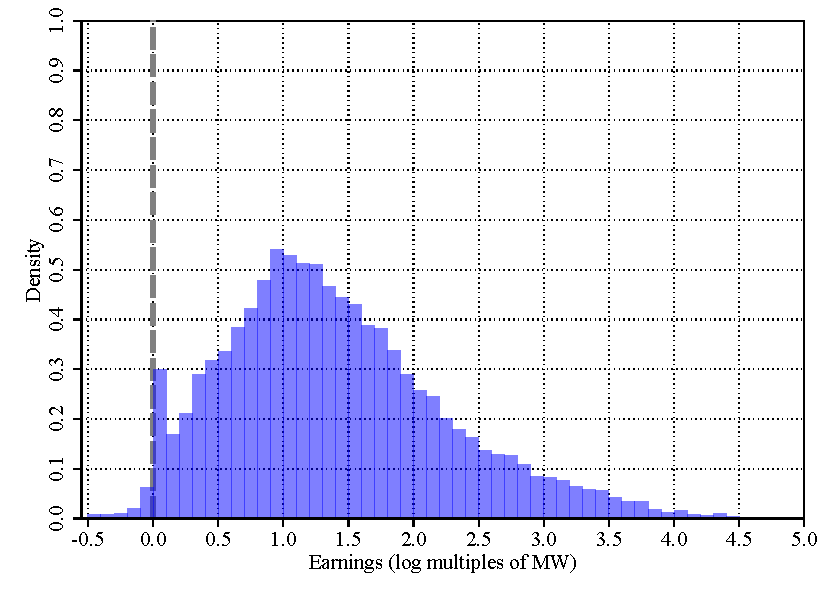
\includegraphics[width=0.33\columnwidth]{_figures/fig1A.pdf}% _figures/hist_spike_ln_1996.pdf
    %
  }
  \subfloat[Histogram of log wages, 2018\label{fig:histograms_log_1996_2018_B}]{%
   \includegraphics[width=0.33\columnwidth]{_figures/fig1B.pdf}% _figures/hist_spike_ln_2018.pdf
    %
  }
  \subfloat[Percentile ratios, 1996--2018\label{fig:histograms_log_1996_2018_C}]{%
   \includegraphics[width=0.33\columnwidth]{_figures/fig1C.pdf}% _figures/inc_p50_p10_inc_p90_p50_short.pdf
    %
  }%
  \\
  %
  \postfigvspace
  %
  \begin{minipage}[t]{1\columnwidth}%
    \begin{spacing}{0.75}
      \emph{\scriptsize{}Notes: }{\scriptsize{}Panels \subref{fig:histograms_log_1996_2018_A} and \subref{fig:histograms_log_1996_2018_B} show histograms of log wages in multiples of the current minimum wage based on 60 equi-spaced bins for population of male workers aged 18--54 for 1996 and 2018, respectively. Panel \subref{fig:histograms_log_1996_2018_C} plots lower- and upper-tail wage inequality, as measured by the P50/P10 and the P90/P50 log wage percentile ratios between 1996 and 2018, normalized to $1.0$ in 1996. %
      \emph{\scriptsize{}Source: } RAIS, 1996--2018.}
    \end{spacing}
  \end{minipage}
  %
\end{figure}




\subsection{Dissecting Brazil's decline in earnings inequality: The role of firms\label{subsec:Motivating-facts}}

To understand the decline in wage inequality in Brazil, we follow \citet{ABEM2018} in implementing a statistical decomposition of wages among formal sector workers in Brazil. Motivated by the fact that a large share of empirical wage dispersion is within detailed worker groups based on observable characteristics---as demonstrated in Appendix \ref{app_subsec:unobserved_heterogeneity}---we estimate two-way fixed effect specifications based on the econometric framework by AKM. The goal of the exercise is to assess whether firms are a key channel through which the distribution of wages may change over time, either through adjustments in firm pay policies or through worker reallocation across firms. Specifically, we decompose log wages $w_{ijt}$ of individual $i$ working at firm $j$ in year $t$ within five-year periods as
%
\begin{equation}
  w_{ijt}=\alpha_{i}+\psi_{j} + X_{it}\beta +\varepsilon_{ijt},\label{eq: AKM framework}
\end{equation}
%
where $\alpha_{i}$ denotes a worker fixed effect, $\psi_{j}$ denotes a firm fixed effect, $X_{it}$ is a vector of time-varying worker characteristics---including education-specific age dummies restricted to be flat between ages 45 and 49, education-specific year dummies, contractual work hours dummies, and six-digit occupation dummies---and $\varepsilon_{ijt}$ is a residual satisfying a strict exogeneity condition. %
%
Equation \eqref{eq: AKM framework} is identified off workers switching employers within the largest set of firms connected through worker mobility. While ordinary least squares (OLS) estimates of individual coefficients in equation \eqref{eq: AKM framework} are unbiased, the variance and covariance terms based on these coefficients generally are biased in finite samples. To correct for this bias, we adopt the leave-one-out estimator developed by KSS, which yields unbiased estimates of the variance components of log wages based on equation \eqref{eq: AKM framework}.%
%
\footnote{There has been a fruitful debate around the benefits and drawbacks of estimating AKM wage equations, including \citet{Andrews2008}, \citet{EeckhoutKircher2011}, \citet{Lopesdemelo2016}, \citet{Card2018}, \citet{BonhommeLamadonManresa2019}, \citet{BonhommeHolzheuLamadonManresaMogstadSetzler2020}, and \citet{Borovickova2020}. In related work, \citet{ABEM2018} and \citet{GerardLagosSeverniniCard2020} present a battery of robustness checks, which suggest that the AKM equation is well suited for describing the Brazilian data during this period.} %
%

Table \ref{TABLE: AKM summary statistics} presents a decomposition of the variance of log wages based on the AKM wage equation \eqref{eq: AKM framework}, separately for a five-year period centered around 1996 (i.e., from 1994--1998) and a five-year period ending in 2018 (i.e., from 2014--2018). For each period, we report results from four estimations: %
%
one without KSS correction and without controls in columns (1) and (5), %
one with KSS correction and without controls in columns (2) and (6), %
one without KSS correction and with controls in columns (3) and (7), and %
one with KSS correction and with controls in columns (4) and (8). %
%
The last four columns report the change between periods for each of the four sets of estimates.

\begin{table}[!htb]
  %
  \centering
  \caption{\label{TABLE: AKM summary statistics}Decomposition of the variance of log wages over time}%
  %
  \pretabvspace
  %
  \resizebox{\textwidth}{!}{%
  \begin{tabular}{lcccccccccccccc}
  \multicolumn{2}{c}{} &  &  &  &  &  &  &  &  &  &  &  &  & \tabularnewline
  \hline
  \hline
   & \multicolumn{4}{c}{Variance (\%), 1994--1998} &  & \multicolumn{4}{c}{Variance (\%), 2014--2018} &  & \multicolumn{4}{c}{Change (\%), 1994--1998 to 2014--2018}\tabularnewline
  \hline
   & (1)  & (2)  & (3)  & (4)  &  & (5)  & (6)  & (7)  & (8)  &  & (5)$-$(1)  & (6)$-$(2)  & (7)$-$(3)  & (8)$-$(4)\tabularnewline
  \hline
  \multicolumn{1}{l}{$Var(w_{ijt})$} & 0.709  & 0.709  & 0.709  & 0.709  &  & 0.444 & 0.444 & 0.444 & 0.444 &  & -0.265 & -0.265 & -0.265 & -0.265\tabularnewline
   & (100\%)  & (100\%)  & (100\%)  & (100\%)  &  & (100\%)  & (100\%)  & (100\%)  & (100\%)  &  & (100\%) & (100\%) & (100\%) & (100\%)\tabularnewline
  $Var(\hat{\alpha}_{i})$  & 0.323  & 0.279  & 0.217  & 0.176  &  & 0.264 & 0.241 & 0.173 & 0.154 &  & -0.059 & -0.038 & -0.044 & -0.022\tabularnewline
   & (46\%)  & (39\%)  & (31\%)  & (25\%)  &  & (59\%) & (54\%) & (39\%) & (35\%) &  & (22\%) & (14\%) & (17\%) & (8\%)\tabularnewline
  $Var(\hat{\psi}_{j})$  & 0.212  & 0.198  & 0.201  & 0.187  &  & 0.083 & 0.076 & 0.078 & 0.072 &  & -0.129 & -0.122 & -0.123 & -0.115\tabularnewline
   & (30\%)  & (28\%)  & (28\%)  & (26\%)  &  & (19\%) & (17\%) & (18\%) & (16\%) &  & (49\%) & (46\%) & (46\%) & (43\%)\tabularnewline
  $2\times Cov(\hat{\alpha}_{i},\hat{\psi}_{j})$  & 0.140  & 0.163  & 0.098  & 0.120  &  & 0.081 & 0.092 & 0.061 & 0.070 &  & -0.059 & -0.071 & -0.037 & -0.050\tabularnewline
   & (20\%)  & (23\%)  & (14\%)  & (17\%)  &  & (18\%) & (21\%) & (14\%) & (16\%) &  & (22\%) & (27\%) & (14\%) & (19\%)\tabularnewline
  $Var(\hat{\varepsilon}_{ijt})$  & 0.034  & 0.070  & 0.033  &  &  & 0.017 & 0.036 & 0.016 &  &  & -0.017 & -0.034 & -0.017 & \tabularnewline
   & (5\%)  & (10\%)  & (5\%)  &  &  & (4\%) & (8\%) & (4\%) &  &  & (6\%) & (13\%) & (6\%) & \tabularnewline
   &  &  &  &  &  &  &  &  &  &  &  &  &  & \tabularnewline
  $Corr\left(\hat{\alpha_{i}},\hat{\psi_{j}}\right)$  & 0.267  & 0.347  & 0.234  & 0.330  &  & 0.273 & 0.340 & 0.263 & 0.332 &  &  &  &  & \tabularnewline
   &  &  &  &  &  &  &  &  &  &  &  &  &  & \tabularnewline
  $R^{2}$  & 0.951  & 0.902  & 0.953  &  &  & 0.961 & 0.919 & 0.965 &  &  &  &  &  & \tabularnewline
  Obs. (mm)  & 67.8  & 67.8  & 67.8  & 67.8  &  & 131.9 & 131.9 & 131.9 & 131.9 &  &  &  &  & \tabularnewline
   &  &  &  &  &  &  &  &  &  &  &  &  &  & \tabularnewline
  KSS correction  & No  & Yes  & No   & Yes  &  & No  & Yes  & No   & Yes  &  & No  & Yes  & No   & Yes\tabularnewline
  Controls        & No  & No   & Yes  & Yes  &  & No  & No   & Yes  & Yes  &  & No  & No   & Yes  & Yes\tabularnewline
  \hline
  \end{tabular}
}

  %
  \posttabvspace
  %
  \begin{minipage}[t]{1\columnwidth}%
    \begin{spacing}{0.75}
      \emph{\scriptsize{}Notes: }{\scriptsize{}This table shows plug-in and bias-corrected variance components of log wages based on estimating AKM equation \eqref{eq: AKM framework} for the population of male workers of age 18--54 in 1994--1998 and 2014--2018. $Var(w_{ijt})$ denotes the variance of log wages, $Var(\hat{\alpha}_{i})$ denotes the variance of estimated person fixed effects, $Var(\hat{\psi}_{j})$ denotes the variance of estimated firm fixed effects, $2\times Cov(\hat{\alpha}_{i},\hat{\psi}_{j})$ denotes two times the sum of the covariance between estimated person fixed effects $\hat{\alpha}_{i}$ and estimated firm fixed effects $\hat{\psi}_{j}$, and $Var(\hat{\varepsilon}_{ijt})$ denotes the variance of estimated residuals. For columns (3)--(4) and (7)--(8), omitted terms include the variance of the estimated component of log wages due to observable worker characteristics, $Var(X_{it}\hat{\beta})$, and two times the sum of covariance terms involving observable worker characteristics. $Corr\left(\hat{\alpha_{i}},\hat{\psi_{j}}\right)$ denotes the correlation between estimated person fixed effects $\alpha_{i}$ and estimated firm fixed effects $\psi_{j}$. Variance shares are in parentheses in columns (1)--(8). Share of total change in the variance of log wages is in parentheses in the last four columns. Observations are in millions of worker-years. KSS correction refers to leave-one-out estimators of variance components by \citet{KlineSaggioSolvsten2020}. The variance of estimated residuals, $Var(\hat{\varepsilon}_{ijt})$, and the coefficient of determination, $R^2$, are not reported in columns (4) and (8) due to their omission in the KSS leave-one-out estimation with controls. Controls include education-specific age dummies restricted to be flat between ages 45 and 49, education-specific year dummies, contractual work hours dummies, and occupation dummies. %
      \emph{\scriptsize{}Source:} RAIS, 1994--1998 and 2014--2018.}
    \end{spacing}
  \end{minipage}
  %
\end{table}

During 1994--1998 (columns 1--4), out of the total variance of wages of 70.9 log points, between 46 and 25 percent are attributable to the variance of person fixed effects. The inclusion of worker controls reduces this share by around one third, while the KSS correction further reduces it. Between 30 percent (column 1) and 26 percent (column 4) of the total variance of log wages are attributed to the firm pay component, with little variation in this share with and without KSS correction or controls. There is significant positive worker-firm sorting, as measured by the correlation between worker and firm fixed effects of 0.330 including the KSS correction and controls. The associated value of two times their covariance term equals 0.120, which accounts for an additional 17 percent of the total variance (column 4).

During 2014--2018 (columns 5--8), the total variance of wages is 44.4 log points, which is 26.5 log points lower relative to 1994--1998. While worker heterogeneity is the most important factor behind the cross-sectional wage variance, a drop in the variance of firm fixed effects constitutes between 49 percent (comparing columns 5 and 1) and 43 percent (comparing columns 8 and 4) of the total decline. A lower variance of person fixed effects accounts for between 22 percent (comparing columns 5 and 1) and 8 percent (comparing columns 8 and 4) of the total decline. Lower covariance terms and residual variance account for the remaining decline. Between the two periods, the correlation between worker and firm fixed effects remained roughly constant, as did the coefficient of determination for the reported specifications.

In summary, Brazil saw a remarkable decline in wage inequality between 1996 and 2018, which was partly driven by a reduction in pay differences across firms for identical workers. We interpret this as evidence for the hypothesis that the decline in inequality over this period was the result of changes in firms' pay policies rather than solely due to changes in worker composition.

% !TEX root = EIMW2022.tex

\section{The minimum wage and other wage setting institutions in Brazil\label{SECTION: Institutions}}

\subsection{Brazil's minimum wage}

Brazil first adopted a regional minimum wage as part of the decree-law \emph{Decreto-Lei No.\ 2.162} on May 1, 1940, under then-dictator and later-elected-president Get{\'{u}}lio Vargas. In 1984, the regional minimum wages were unified under a federal minimum wage. %
%
Over much of the period we study, the federal minimum wage was the only unconditional wage floor in place. However, since the passage of the labor law \emph{Lei Complementar No.\ 103} on July 14, 2000, states are allowed to institute their own wage floors called \emph{Pisos Salariais Estaduais}. Since then, five out of the 27 states have instituted such state-specific minimum wages \citep{CorseuilFogelHecksher2015,SaltielUrzua2020}.%
%
\footnote{Technically, the Federative Republic of Brazil consists of 26 states and one federal district, the \emph{Distrito Federal}. For simplicity, we henceforth refer to all of Brazil's 27 federative units (i.e., the 26 states and the federal district) as ``states.''} %
%
These five states are located in the relatively high-income southern and southeastern regions of Brazil and comprise Rio de Janeiro and Rio Grande do Sul since 2001, Paran{\'{a}} since 2006, S{\~{a}}o Paulo since 2007, and Santa Catarina since 2010. %
%
Nevertheless, the federal minimum wage (henceforth referred to as the ``minimum wage'') remains the most important wage floor for the majority of the Brazilian population.

Brazil's minimum wage is stated in terms of a floor on monthly nominal earnings, with no provisions for legal subminimum wages or differentiated minimum wages across demographics or economic subdivisions \citep{Lemos2004}. The minimum wage applies to workers with full-time contracts of 44 hours per week, and is adjusted proportionately for part-time workers.%
%
\footnote{Using information on hours in the RAIS data, we find a relatively small share of part-time workers. Special labor contracts allow for parts of the minimum wage to be paid in-kind in the form of accommodation
and food, although in the PNAD data only 0.8 percent of workers report receiving nonmonetary remuneration in 1996.} %


\subsection{Other wage setting institutions}

While the minimum wage serves as an important reference point for wage setting in Brazil, a number of other labor market institutions complement its role. Industry- and occupation-specific trade unions regularly negotiate wage floors for members and other workers with coverage of collective bargaining agreements. During the hyperinflationary period of the early 1990s, wages were commonly expressed as multiples of the minimum wage, though its use as an explicit numeraire has been outlawed and, in practice, is greatly imperfect. Nevertheless, the minimum wage serves as a benchmark for unemployment and retirement benefits. Apart from providing a lower bound on permissible wages, the minimum leaves ample freedom for firms to pay above the minimum wage. In this way, the minimum wage serves as a reference point for wage negotiations.

\subsection{\label{subsec:The-minimum-wage}Evolution of Brazil's minimum wage over time}

Motivated by the remarkable decline in wage inequality in Brazil, we now turn to a
salient change in the labor market over this period: the rise in the
minimum wage.%
%
\footnote{While Brazil enacted other social policies during the mid-2000s, such as a transfer program for needy families (\emph{Bolsa Fam{\'{i}}lia}) launched in 2003, the minimum wage predates many of these policies.} %
%
Brazil's real minimum wage deteriorated under high inflation between 1985 and 1995. A switch in government towards the end of this period ignited a gradual ascent of the wage floor from BRL 500.4 in 1996 to BRL 1,142.3 (both in constant September 2021 BRL) in 2018, which corresponds to a 128.3 percent increase in real terms. Accounting for aggregate productivity growth, this corresponds to a 58.6 log points real productivity-adjusted rise in the minimum wage over 23 years. To put these numbers into context, the minimum wage as a fraction of the median wage increased from around 30.3 percent in 1996 to around 55.6 percent in 2018. Figure \ref{fig:var_minw_short} shows a strong negative comovement between the minimum wage and the standard deviation of log wages between 1996 and 2018, with a time series correlation of $-0.973$.%
%
\footnote{Appendix \ref{appendix: inequality and mw} shows an equally striking comovement between earnings inequality and the minimum wage over the extended period from 1985--2018.} %

\begin{figure}[!htb]
  %
  \centering
  \caption{\label{fig:var_minw_short}Evolution of wage inequality and the real minimum wage}
  %
  \prefigvspace
  %
  \includegraphics[width=0.45\columnwidth]{_figures/fig2.pdf} % _figures/sd_mw_real_short.pdf
  %
  \\
  %
  \postfigvspace
  %
  \begin{minipage}[t]{1\columnwidth}%
    \begin{spacing}{0.75}
      \emph{\scriptsize{}Notes: }{\scriptsize{}Statistics are for males
      of age 18--54. Real minimum wage is the annual mean of the monthly
      time series. The correlation between the two time series is $-0.973$. %
      \emph{\scriptsize{}Source: } RAIS and IPEA, 1996--2018.}
    \end{spacing}
  \end{minipage}
  %
\end{figure}

% !TEX root = EIMW2022.tex

\section{Cross-sectional heterogeneity and the minimum wage\label{SECTION: Empirics}}

While the correlation between the minimum wage and aggregate wage inequality documented in the previous section is striking, we caution against interpreting this pattern as causal. For example, the changes in wage inequality over this period might have been driven by simultaneous changes in macroeconomic conditions or secular trends in the wage distribution unrelated to Brazil's federal minimum wage. We address this simultaneity problem by exploiting spatial variation in the bindingness of the federal minimum wage across states in Brazil, building on the seminal econometric framework by \citet{Lee1999} and the recent contribution by \citet{Autor2016}. This approach allows us to filter out changes in national macroeconomic conditions and secular trends. In this sense, the fact that inequality decreased in Brazil over this period is neither necessary nor sufficient for our conclusions regarding the effects of the minimum wage on wage inequality.


\subsection{Motivating evidence on state-level heterogeneity}

To motivate our econometric analysis, we start by noting that wage inequality---while declining overall during this period---fell disproportionately in initially lower-income regions for which the federal minimum wage was relatively more binding. Figure \ref{fig:Inequality_evolution} plots normalized wage inequality measures between 1996 and 2018 for the three lowest-income states and three highest-income states in Brazil in 1996.%
%
\footnote{The three low-income states are Maranh{\~{a}}o, Piau{\'{i}}, and Para{\'{i}}ba, while the three high-income states are Rio de Janeiro, S{\~{a}}o Paulo, and Distrito Federal.} %
%
Panel \subref{subfig:Inequality_evolution_A} shows that the variance of log wages drops by more than half in initially low-income states, but by less than one-fifth in initially high-income states. Panel \subref{subfig:Inequality_evolution_B} shows that lower-tail inequality drops especially in initially low-income states, with the P50--P10 and P50--P25 for this group declining by 50 and 40 percent, respectively, but by markedly less for initially high-income states. In contrast, upper-tail inequality, measured by the P75--P50 or the P90--P50, falls only in initially low-income states, as shown in panel \subref{subfig:Inequality_evolution_C}.%
%
\footnote{Appendix \ref{app_subsection:lee_regressions} shows that the inverse relationship between the effective bindingness of the minimum wage and wage inequality generalizes to the full set of states.} %
%

These empirical patterns yield three take-aways. First, Brazil's inequality decline was due to factors that matter more at lower income levels. Second, the inequality decline was associated with compression particularly in the bottom of the wage distribution. Third, the compression in the wage distribution reaches from the bottom to above the median of the wage distribution. This motivates our study of the minimum wage.


\begin{figure}[!htb]
  %
  \centering
  \caption{\label{fig:Inequality_evolution}Evolution of wage inequality across rich and poor states}
  %
  \prefigvspace
  %
  \subfloat[Overall inequality\label{subfig:Inequality_evolution_A}]{%
   \includegraphics[width=0.33\columnwidth]{_figures/fig3A.pdf}% _figures/comp_sd_1996_2018.pdf
    %
  }
  \subfloat[Lower-tail inequality\label{subfig:Inequality_evolution_B}]{%
   \includegraphics[width=0.33\columnwidth]{_figures/fig3B.pdf}% _figures/comp_percentiles_bottom_1996_2018.pdf
    %
  }
  \subfloat[Upper-tail inequality\label{subfig:Inequality_evolution_C}]{%
   \includegraphics[width=0.33\columnwidth]{_figures/fig3C.pdf}% _figures/comp_percentiles_top_1996_2018.pdf
    %
  }%
  \\
  %
  \postfigvspace
  %
  \begin{minipage}[t]{1\columnwidth}%
    \begin{spacing}{0.75}
      \emph{\scriptsize{}Notes: }{\scriptsize{}For this figure, we assign the three lowest-income states and three highest-income
      states states in Brazil in 1996 into a ``low income'' group and a ``high income'' group, respectively. The three low-income states are Maranh{\~{a}}o, Piau{\'{i}}, and Para{\'{i}}ba, while the three high-income states are Rio de Janeiro, S{\~{a}}o Paulo, and Distrito Federal. The three panels then plot various wage inequality measures by state group between 1996 and 2018, normalized to $1.0$ in 1996.
      panel \subref{subfig:Inequality_evolution_A} shows the variance
      of log wages, panel \subref{subfig:Inequality_evolution_B} shows
      lower-tail percentile ratios (P50/P10 and P50/P25) of log wages, and panel \subref{subfig:Inequality_evolution_C}
      shows upper-tail percentile ratios (P75/P50 and P90/P50) of log wages. %
      \emph{\scriptsize{}Source: } RAIS, 1996--2018.}
    \end{spacing}
  \end{minipage}
  %
\end{figure}




\subsection{Econometric framework\label{subsec:Spillover-effects-identified}}

To correlate the minimum wage with wage inequality, we follow \citet{Lee1999} and \citet{Autor2016} in exploiting heterogeneous exposure across states that differ in their bindingness with respect to Brazil's federal minimum wage. To this end, we define the \emph{Kaitz-$p$ index} for state $s$ in year $t$ as $kaitz_{st}(p) \equiv \log w_{t}^{min} - \log w_{st}^{\text{P}p}$. That is, the Kaitz-$p$ index is the log difference between the federal minimum wage prevailing in year $t$, $w_{t}^{min}$, and the $p$th percentile of the log wage distribution of state $s$ in year $t$, $w_{st}^{\text{P}p}$.%
%
\footnote{Figure \ref{fig: kaitz} in Appendix \ref{subsec:kaitz-evolution} shows that variation across Brazilian states in the Kaitz-$p$ index, for $p \in \{ 50, 90 \}$, is large initially and decreases as the minimum wage increases, while approximately preserving the ranking of states over time.} %
%
We are interested in how various inequality measures at the state-year level covary with the Kaitz-$p$ index, for high enough $p$ such that the $p$th percentile of the wage distribution is not (directly or indirectly) affected by the minimum wage. To assess this, we regress outcome variable $y_{st}(p';p)$ specific to wage percentile $p'$ with respect to some base percentile $p$ in state $s$ and year $t$ on the Kaitz-$p$ index, using the same base percentile $p$, and state-year controls:
%
\begin{align}
  y_{st}(p';p) &= \sum_{n=1}^{N} \beta_{n}(p') \times kaitz_{st}(p)^{n} + \gamma_{s}(p') + \delta_{s}(p') \times t + \varepsilon_{st}(p'),\label{eq:Lee}
\end{align}
%
where $y_{st}(p';p)$ may stand in for the log ratio of wage percentile $p'$ over wage percentile $p$ in state $s$ and year $t$, $N$ denotes the order of the polynomial in the Kaitz-$p$ index, $\beta_{n}(p')$ is the percentile $p'$-specific coefficient on the $n$th power of the Kaitz-$p$ index, $\gamma_{s}(p')$ is a set of state dummies for each percentile $p'$, and $\delta_{s}(p') \times t$ is a set of state-specific linear time trends for each percentile $p'$. Finally, $\varepsilon_{st}(p')$ is a percentile $p'$-specific error term, which we assume satisfies the strict exogeneity condition $\mathbb{E}[\varepsilon_{st}(p')|kaitz_{st}(p),\ldots,kaitz_{st}(p)^{n},\gamma_{s}(p'), \delta_{s}(p') \times t]=0$.

After estimating equation \eqref{eq:Lee} separately for each wage percentile $p'$ using a baseline percentile $p$, we estimate the marginal effect of the minimum wage throughout the wage distribution,
%
\begin{equation}
    \rho(p',p) \equiv \sum_{n=1}^{N}n\beta_{n}(p') \times kaitz_{st}(p)^{n-1},\label{eq:Lee_marginal_effect}
\end{equation}
%
evaluated at the worker-weighted median value of the Kaitz-$p$ index across states and years. Allowing for polynomials of order $N \ge 2$ is important to capture the nonlinear effects of the minimum wage as it becomes more binding. After trying different values, we set $N=2$.%
%
\footnote{Using polynomials of order $N>2$ yields results that are substantially the same as those presented below.} %
%

We first consider as outcome variables in equation \eqref{eq:Lee} a set of global or local wage inequality measures. To capture the effects of the minimum wage on global wage inequality, we consider a variant of equation \eqref{eq:Lee} that uses the standard deviation of log wages as the dependent variable. To capture the effects of the minimum wage on local wage inequality, we use---for various values of $p' \in \{ 10, 15, \ldots, 90 \}$---the log ratio between wage percentile $p'$ and a base percentile $p$, so that $y_{st}(p';p)=\log [ w_{st}(p') / w_{st}(p) ]$. Here, $p$ is the same percentile as in the Kaitz-$p$ index. Ideally, $p$ would be chosen high enough so as to be (directly and indirectly) unaffected by the minimum wage. Prior studies of the minimum wage in the U.S. context have used $p=50$---i.e., the median---while appealing to the fact that, ex-post, their findings suggest insignificant spillover effects at or above that point in the wage distribution. For Brazil, where the minimum wage is more binding than in the U.S., we report results for the same value of $p=50$ and consistently find a statistically significant correlation with outcomes above the median of the wage distribution.%
%
\footnote{See Appendix \ref{app_subsec:comparison_Brazil_US} for a comparison of the relative bindingness of the minimum wage, as proxied by left-tail wage inequality, between Brazil and the U.S.} %
%
Therefore, we also report results for an alternative, preferred normalization using $p=90$.

When analyzing the correlation between the minimum wage and log wage percentile ratios, the inclusion of the $p$th wage percentile in both the dependent and the independent variable may induce a spurious correlation that results in biased estimates of the coefficient $\beta_{n}(p')$, and thus the marginal effect $\rho(p',p)$, in the presence of measurement error or other transitory shocks \citep{Autor2016}. While measurement error is plausibly a lesser concern in large administrative data such as ours, we address this issue by implementing a variant of the solution proposed by \citet{Autor2016}. Specifically, we adopt an instrumental variables (IV) strategy that predicts the Kaitz-$p$ index and its square based on an instrument set that consists of the log real statutory minimum wage, its square, and the log real statutory minimum wage interacted with the mean of the log real $p$th percentile of the wage distribution for each state over the full sample period. The motivation for this instrument set is that the current level of the statutory minimum wage in relation to the long-term average income level within a state affects the concurrent bindingness of the minimum wage (i.e., instrument relevance) and has an effect on concurrent wage inequality only through its effect on the concurrent bindingness of the minimum wage (i.e., the exclusion restriction) by being essentially decoupled from transitory wage fluctuations. Since we study states' differential exposure to the federal minimum wage, rather than state-level minimum wages that are more likely to be endogenous to local economic conditions, we include as controls in our IV specification state-specific linear time trends instead of a set of year dummies as in \citet{Autor2016}.


\paragraph{Result 1: Effects of the minimum wage on wage inequality.}

Figure \ref{fig:Lee_regression} shows the results obtained from estimating equation \eqref{eq:Lee} over the sample period from 1996 to 2018. We report results for our baseline specifications with state fixed effects and state-specific linear time trends, estimated via OLS in levels across Brazil's 27 states, with the base percentile being either $p=50$ (panel \subref{fig:Lee_regression_A}) or $p=90$ (panel \subref{fig:Lee_regression_B}). The shaded areas represent 99 percent confidence intervals based on regular (i.e., not clustered) standard errors. In each panel, we report the estimated marginal effect on the standard deviation of log wages (``St.d.'' on the x-axis) and on wages between the 10th and the 90th percentiles of the wage distribution (``10'' to ``90'' on the x-axis) relative to the base wage $p$.


\begin{figure}[!htb]
  %
  \centering
  \caption{\label{fig:Lee_regression}Estimated minimum wage effects on the distribution of wages}
  %
  \prefigvspace
  %
  \hspace*{\fill}%
  \csubfloat[Relative to P50\label{fig:Lee_regression_A}]{%
   \includegraphics[width=0.45\columnwidth]{_figures/fig4A.pdf}% _figures/baseline_p50_1996_2018.pdf
  }\centerhfill[\qquad\qquad\qquad\qquad\qquad]
  \csubfloat[Relative to P90\label{fig:Lee_regression_B}]{%
   \includegraphics[width=0.45\columnwidth]{_figures/fig4B.pdf}% _figures/baseline_p90_1996_2018.pdf
  }\hspace*{\fill}
  %
  \\
  %
  \postfigvspace
  %
  \begin{minipage}[t]{1\columnwidth}%
    \begin{spacing}{0.75}
      \emph{\scriptsize{}Notes:}{\scriptsize{} Figure plots estimated marginal effects from equation \eqref{eq:Lee_marginal_effect} based on the regression framework in equation \eqref{eq:Lee}. Each panel shows the results from a baseline specification, with estimated marginal effects shown as black circles connected by lines and standard error bands shown as bars or shaded areas. The baseline specification includes state fixed effects in addition to state-specific linear time trends and is estimated using ordinary least squares (OLS). Each value on the horizontal axis corresponds to a separate regression for a specific dependent variable, which can be either the standard deviation of log wages (``St.d.'' on the x-axis) or wages between the 10th and the 90th percentiles of the wage distribution (``10'' to ``90'' on the x-axis) relative to some base wage $p$. Panel \subref{fig:Lee_regression_A} uses the 50th percentile as the base wage (i.e., $p=50$), while panels \subref{fig:Lee_regression_B} uses the 90th percentile as the base wage (i.e., $p=90$). Both panels are estimated across Brazil's 27 states. The bars and four shaded areas represent 99 percent confidence intervals based on regular (i.e., not clustered) standard errors. %
      \emph{\scriptsize{}Source: } RAIS, 1996--2018.}
    \end{spacing}
  \end{minipage}
  %
\end{figure}


The results show a strong correlation between the minimum wage and inequality throughout the wage distribution. Using the median as a base percentile (panel \subref{fig:Lee_regression_A}), the estimated marginal effects of the minimum wage are monotonically decreasing between the 10th and the 75th percentile, and statistically significant at the one percent level throughout. The marginal effects are also tightly estimated.

The statistically significant correlation between the minimum wage and inequality outcomes above the median motivates our alternative normalization using the 90th wage percentile (panel \subref{fig:Lee_regression_B}). Inspecting these results, we estimate monotonically decreasing and statistically significant marginal effects of the minimum wage up to the 90th percentile. Again, the marginal effects are tightly estimated.

In terms of the correlation between the minimum wage and the standard deviation of log wages, our estimates across the two base wages in panels \subref{fig:Lee_regression_A} and \subref{fig:Lee_regression_B} of Figure \ref{fig:Lee_regression} yield consistent results, with an estimated semi-elasticity of around -0.20. This means that a one percent increase in the nominal minimum wage, holding fixed the median 90th percentile of wages, is associated with a decrease in the standard deviation of wages of around 20 log points. Although caution is warranted when extrapolating from cross-sectional regressions to aggregate trends, these estimates suggest a decline in the standard deviation of wages of around 11.7 log points, compared to the actual decline in the standard deviation of wages of 19.3 log points in the raw data, in response to the 58.6 log point labor productivity-adjusted increase in the minimum wage seen in Brazil between 1996 and 2018.

We conduct a battery of robustness checks and consistently find that spillovers reach up to or above the 75th percentile of the earnings distribution. This is significantly higher than previous evidence on the reach of minimum wage spillovers in the US due to \citet{Lee1999}, who finds significant effects up to the median of the wage distribution, and \citet{Autor2016}, who find spillovers in the lowest quintile of the wage distribution. Importantly, \citet{Autor2016}'s concern that measurement error may bias estimates of the effect of the minimum wage does not seem to drive our finding, as Appendix \ref{app_subsec_alt_specs} shows by presenting similar results from the IV specification described above.%
%
\footnote{Appendix \ref{app_subsec_alt_specs} also shows similar results from OLS and IV specifications in differences, though with significantly larger standard error bounds. In Appendix \ref{app_subsec_alt_controls}, we find similar results using alternative sets of controls, including only state fixed effects, only year fixed effects, state and year fixed effects, and state and year fixed effects in addition to state-specific linear trends. Appendix \ref{app_subsec_alt_periods} shows that these results are not unique to the 1996--2018 period we study, since we find similar results for the period 1985--2007 and the complete set of years 1985--2018. Notably, spillover effects are not markedly stronger during the early period of 1985--1995, though the right tail of our estimates suggests that there were significant transitory state-level shocks not related to the minimum wage during this high-inflation period. Appendix \ref{app_subsec:lee_regressions_trends} shows similarly strong spillover effects when controlling for state-specific quadratic or cubic time trends. Although the number of states (27) falls below conventional thresholds for clustering \citep{CameronMiller2015}, Appendix \ref{app_subsec:lee_regressions_cluster} also presents results with standard errors clustered at the state level and a separate specification estimated at the level of mesoregions (of which there are 137) with standard errors clustered at the mesoregion level. Finally, in Appendix \ref{app_subsec:lee_regressions_haanwinckel} we show that similar insights are obtained from a set of specifications and controls replicating those in complementary work by \citet{Haanwinckel2020}, the relation to which we discuss in some detail in Appendix \ref{app_subsec:lee_regressions_haanwinckel}.} %
%
In this way, our results complement recent evidence by \citet{FortinLemieuxLloyd2021} that relies on a method robust to the type of measurement error problem described in \citet{Autor2016} and finds spillover effects similar to those of \citet{Lee1999} for the same period of the 1980s in the US.

Our robust finding of a correlation between the minimum wage and inequality outcomes up to the 90th percentile of the wage distribution may seem surprising. For comparison, \citet{Autor2016} show spillovers up to the 20th percentile of the wage distribution in the U.S. In light of this, we make five observations. First, our large-scale administrative data plausibly admit less measurement error than the CPS, alleviating concerns about bias in the estimates of $\beta_{n}(p)$ in equation \eqref{eq:Lee} and allowing us to measure spillover effects with greater accuracy than previously possible. %
Second, the minimum wage in Brazil during this period was more binding compared to that in the U.S. over the last decades \citep{Autor2016}, which due to the nonlinear nature of spillover effects is expected to lead to greater effects throughout the wage distribution.%
%
\footnote{Appendix \ref{app_subsec:comparison_Brazil_US} shows that between 1996 and 2018, the minimum wage in Brazil relative to that in the U.S. has gone from less binding to significantly more binding.} %
%
Third, while a relatively small fraction of Brazilian workers earn the minimum wage in any given year during our sample period, we find that a significant fraction of workers throughout the wage distribution ever (currently, in the past, or in the future) earn the minimum wage during our sample period. This may suggest that the minimum wage in Brazil acts as an important stepping stone, even for workers that eventually find themselves high up in the wage distribution.%
%
\footnote{Appendix \ref{app:mw_spike} shows that a relatively small fraction of Brazilian workers have wages exactly equal to, less than, or around the minimum wage at any given point in time between 1996 and 2018. Appendix \ref{appendix:who_earns_the_mw} studies characteristics of minimum wage earners.} %
%
Fourth, the minimum wage in Brazil is particularly salient given Brazil's volatile economic history. While indexation of wages to the minimum wage is not allowed by Brazilian labor laws and not supported by the government, the minimum wage still serves as an important reference point in wage setting mechanisms \citep{NeriMoura2006}.%
%
\footnote{Our model in Section \ref{SECTION: Model} rationalizes the view of the minimum wage as a reference point as an equilibrium outcome due to frictional inter-firm competition for workers. In the data, like in our model, the link between the minimum wage and the wage distribution is imperfect---not all wages move one-for-one with the minimum wage. Thus, the wage distribution compresses as the minimum wage is increased. Appendix \ref{app_subsec:comparison_nominal_multiples} compares the distribution of (changes in) wages in nominal values and in multiples of the current minimum wage.} %
%
Fifth and finally, compared to the U.S., Brazil's workforce is heavily skewed toward low-skill workers as measured by educational attainment. It is around the 75th--90th percentile of the wage distribution where there is a sharp increase in the share of workers with either a high school or a college degree, and also where (log) wages increase sharply across wage quantiles.%
%
\footnote{See Appendix \ref{subsec:Summary-statistics} for details.} %
%
Therefore, we would naturally expect the minimum wage to have a greater impact among lower-skill workers, which make up a relatively larger population share in Brazil compared to the U.S.


\paragraph{Result 2: Effects of the minimum wage on employment.}

So far, we have focused on the correlation between the minimum wage and inequality. We now extend our regression framework to investigate the link between the minimum wage and employment outcomes---including formal and informal sectors---over our period of study. To this end, we supplement the administrative data from RAIS with household survey data from PNAD and PME, based on which we estimate variants of the specification in equation \eqref{eq:Lee} with a dependent variable $y_{st}$ that captures employment outcomes at the region-year level.
%
\footnote{A region corresponds to Brazil's 27 states in RAIS and PNAD and to one of the six largest metropolitan areas in PME.} %
%
For simplicity, we present results based on specifications that use the Kaitz-50 index, though we obtain similar results when using the Kaitz-90 index.

Consistent with previous evidence by \citet{Lemos2009}, results from the PNAD survey data in panel A in Table \ref{tab:employment_effects} show that the minimum wage has precisely estimated zero effects on the population size, labor force participation rate, employment rate, and formal employment share, all of which are insignificant at conventional levels. Specifically, there is little evidence of cross-state differences in population or labor force dynamics linked to the minimum wage---if anything, the rise in the minimum wage is associated with a rise in log population size that is statistically significant only at the ten percent level. Results from the PME data in panel B show small estimated marginal effects of the minimum wage on transition rates from nonformal to formal as well as from formal to nonformal employment. While both point estimates are negative, they are also statistically insignificant at conventional levels.%
%
\footnote{An increase in the minimum wage may affect both formal and informal employment, as studied by \citet{Jales2018}. Unfortunately, the condition of no spillover effects imposed by \citet{Jales2018} does not hold in our context.}
%
Finally, panel C shows the estimated effects of the minimum wage on other labor market outcomes in RAIS. Mean hours worked show a significant correlation of mild magnitude with the relative bindingness of the minimum wage, suggesting that the intensive margin of hours adjustments in response to the minimum wage \citep{Doppelt2019} is not of prime importance in the Brazilian context. Mean firm size correlates strongly positively with the minimum wage, consistent with the idea that the minimum wage induces small firms to shrink or exit in favor of larger competitors. The estimated effect on the probability of remaining employed at the same firm until next year is negative and significant, suggesting that some jobs are destroyed as the minimum wage increases. However, together with our findings of constant labor force participation, employment, and formality rates in response to the minimum wage increase, this suggests that the effect of the minimum wage is primarily to reallocate workers across firms rather than a reduction in overall employment.%
%
\footnote{See also Appendix \ref{sec:Hours} for a more detailed analysis of the correlation between the minimum wage and hours worked.} %
%

\begin{table}[!htb]
  %
  \centering
  \caption{\label{tab:employment_effects}Effects of the minimum wage on employment worker transitions}
  %
  \pretabvspace
  %
  \begin{tabular}{lc}
  \multicolumn{1}{c}{} & \tabularnewline
  \hline
  \hline
   & Marginal effect (standard error)\tabularnewline
  \hline
  \multicolumn{2}{l}{\emph{Panel A. Cross-sectional household survey data (PNAD)}}\tabularnewline
  Log population size & \hphantom{$-$}0.057 (0.030)\tabularnewline
  Labor force participation rate & \hphantom{$-$}0.009 (0.016)\tabularnewline
  Employment rate & \hphantom{$-$}0.014 (0.015)\tabularnewline
  Formal employment share & \hphantom{$-$}0.024 (0.020)\tabularnewline
   & \tabularnewline
  \multicolumn{2}{l}{\emph{Panel B. Longitudinal household survey data (PME)}}\tabularnewline
  Transition rate nonformal-formal & $-$0.003 (0.017)\tabularnewline
  Transition rate formal-nonformal & $-$0.005 (0.009)\tabularnewline
   & \tabularnewline
  \multicolumn{2}{l}{\emph{Panel C. Administrative linked employer-employee data (RAIS)}}\tabularnewline
  Mean log hours worked & \hphantom{$-$}0.043 (0.003)\tabularnewline
  Mean log firm size & \hphantom{$-$}0.433 (0.055)\tabularnewline
  Probability of remaining employed at the same firm until next year & $-$0.111 (0.011)\tabularnewline
  \hline
\end{tabular}

  %
  \posttabvspace
  %
  \begin{minipage}[t]{1\columnwidth}%
    \begin{spacing}{0.75}
      \emph{\scriptsize{}Notes:}{\scriptsize{} This table shows the predicted marginal
      effects with standard errors in parentheses evaluated at the worker-weighted
      mean across Brazil's 27 states. Each cell corresponds to the estimated coefficient and standard error from one regression with the relevant dependent variable (row). The underlying regressions are variants of equation \eqref{eq:Lee} including state fixed effects and state-specific linear time trends. %
      \emph{\scriptsize{}Source: } PNAD, 1996--2012, PME, 2002--2012, and RAIS, 1996--2018.}
    \end{spacing}
  \end{minipage}
  %
\end{table}




\subsection{A call for an equilibrium model\label{subsec:data_to_model}}

The above findings suggest that Brazil's minimum wage has had far-reaching effects on the wage distribution. That the inequality-decreasing effects of the minimum wage are so large may seem surprising in light of past findings of smaller effects in the U.S. by \citet{Lee1999} and \citet{Autor2016}. Yet there exists little theoretical guidance on how strong we should expect spillover effects of the minimum wage to be and at what cost they may come. Furthermore, reduced-form estimates based on cross-sectional variation recover only the relative, but not the absolute, effects of the minimum wage---a problem that is compounded if spillovers are present throughout most of the wage distribution.%
%
\footnote{This is a variant of the ``missing intercept'' problem highlighted in a recent micro-to-macro literature \citep{NakamuraSteinsson2018}.} %
%
Finally, there may remain concerns about confounding factors not controlled for in our econometric analysis, such as the concurrent rollout of social security programs and the expansion of education in Brazil.

To address these issues, we develop and estimate an equilibrium model of the Brazilian labor market subject to a minimum wage. Such a model, while based on certain assumptions, can lend additional credibility to our reduced-form estimates, which rely on a very different set of assumptions. Another benefit of a structural model is that it can aggregate the effects of the minimum wage estimated based on cross-sectional variation in the data, while shedding light on the mechanisms by which the minimum wage impacts the labor market through counterfactual simulations.

% !TEX root = EIMW2022.tex

\section{Equilibrium model of a labor market subject to a minimum wage\label{SECTION: Model}}

We now develop an equilibrium model of the Brazilian labor market subject to a minimum wage. Our framework is essentially a series of heterogeneous \citet{BurdettMortensen1998} economies separated by worker types. Our contribution is to provide empirical content to this framework by integrating unobserved worker heterogeneity, minimum wage jobs, and endogenous job creation in a tractable manner. The extended framework is geared toward estimation on linked employer-employee data and an analysis of the equilibrium effects of the minimum wage on the distribution of wages and employment. %

\subsection{Environment}

Consider a continuous-time economy in steady state populated by a unit mass of workers and a mass $M$ of firms, both infinitely-lived and with risk-neutral preferences over consumption discounted at rate $\rho$.


\paragraph{Worker types.}

At any point in time, a worker can be either employed or nonemployed. We think of nonemployment as a simple way of capturing either unemployment or informal employment with associated utility flow value $ab(a)$ that depends on permanent worker ability $a \sim \Psi(\cdot)$, with $a \in [\underline{a},\overline{a}]$. That the informal market offers a constant flow utility simplifies the analysis substantially. We think of the dependence of this flow utility on ability $a$ as reflecting individual traits that are valued not just in formal employment but also in informal employment or home production. This ability parameter corresponds to both observable and unobservable worker characteristics, which Appendix \ref{app_subsec:unobserved_heterogeneity} shows matter for explaining empirical wage dispersion.

Workers also differ in their relative on-the-job search efficiency, $s\in[\underline{s},\overline{s}]$. In particular, an employed worker of type $(a,s)$ becomes nonemployed at Poisson rate $\delta(a,s)$, at which point her search efficiency is updated according to a first-order Markov process with transition probability $\pi(s'|a,s)$.\footnote{The assumption that search efficiency only updates when a worker transitions into nonemployment avoids added complexity from worker type transition hazards entering firms' problem.} We think of this assumption as reflecting in reduced-form different propensities to switch employers, for instance due to family circumstances preventing a geographic move.\footnote{In a framework with endogenous search intensity as in \citet{Lentz2010}, we hypothesize that a rise in the minimum wage would have two opposing effects on incentives to search. On the one hand, it would render employment more attractive since it pays better on average, which incentivizes search. On the other hand, it flattens the wage ladder and reduces job vacancies, which disincentivizes search. Given these offsetting forces and existing evidence that worker search effort is rather inelastic \citep{engbom2020}, we focus here on a model with exogenous search effort.} %
As will become clear, it allows the model to match the modest spike in the wage distribution at the minimum wage in Brazil (that being said, we show in Appendix \ref{app_subsec:effects_dependence_on_parameters} that our main results are not sensitive to the particular value for $\pi(s'|a,s)$).

\paragraph{Technology.}

Firms are heterogeneous in their permanent productivity $z \sim \Gamma(z)$, with $z \in [\underline{z},\overline{z}]$. A firm that employs $l(a,s)$ workers of each type $(a,s)$ produces output according to the linear technology
%
\begin{eqnarray*}
  y\left(z,\left\{ l(a,s)\right\} _{a,s}\right) &=& z\int_{\underline{a},\underline{s}}^{\overline{a},\overline{s}} a l(a,s)da ds.
\end{eqnarray*}
%
To hire workers, firms post vacancies $v$ in each market $(a,s)$ at a strictly convex, increasing cost $c(v|a,s)$, which reflects the cost of advertising the job, screening applicants and training workers for the job.


\paragraph{Search and matching.}

Both nonemployed and employed workers search for jobs at random in labor markets that are segmented by worker type, $(a,s)$. Let $p(a,s)$ denote the Poisson arrival rate of job offers per unit of search efficiency in market $(a,s)$. A job offer is an opportunity to work for a fixed piece rate $w$ for the duration of a job. Therefore, a worker of ability $a$ employed at piece rate $w$ receives flow value $wa$. Let $F(w|a,s)$ denote the cumulative distribution function (cdf) of piece rates offered in market $(a,s)$. While workers take offer arrival rates and the offer distribution as given, both are determined in equilibrium by firms' vacancy and wage posting decisions. In particular, if firms post total vacancies $V(a,s)$ in a given market $(a,s)$ and workers's aggregate search intensity is $S(a,s) = u(a,s)+se(a,s)$, where $u(a,s)$ is the number of nonemployed workers and $e(a,s)$ is the number of employed workers of type $(a,s)$, then the total number of worker-firm contacts in market $(a,s)$ is given by $\chi V(a,s)^{\alpha}S(a,s)^{1-\alpha}$. Here, $\chi>0$ is the match efficiency and $\alpha\in(0,1)$ is the match elasticity with respect to aggregate vacancies.




\subsection{Worker's problem and the distribution of workers over the job ladder}

Let $U(a,s)$ denote the value to an nonemployed worker with ability $a$ and search efficiency $s$. Let $W(w,a,s)$ be the value to a worker with ability $a$ and search efficiency $s$ from being employed at piece rate $w$. The value $U(a,s)$ satisfies the following Hamilton-Jacobi-Bellman (HJB) equation:
%
\begin{eqnarray}
  \label{eq: value of unemployment}
  \rho U\left(a,s\right) &=& a b\left(a\right) + p(a,s)\int_{\underline{w}(a,s)}^{\overline{w}(a,s)}\max\left\{ W(w,a,s)-U\left(a,s\right),0\right\} dF\left(w\left|a,s\right.\right)
\end{eqnarray}
%
For nonemployed workers, there exists a reservation threshold $r(a,s)$ such that $W(r(a,s),a,s)=U\left(a,s\right)$. A nonemployed worker of type $(a,s)$ accepts any piece rate offer $w \geq r(a,s)$ and rejects any offer $w < r(a,s)$. In equilibrium, firms only make offers with $w \geq r(a,s)$.

The value $W(w,a,s)$ of a worker of type $(a,s)$ employed at piece rate $w$ is given by the HJB equation:
%
\begin{eqnarray}
  \label{eq: value of employment}
  \rho W(w,a,s)	&=& wa + sp(a,s)\int_{w}^{\overline{w}(a,s)}\left(W\left(w',a,s\right)-W\left(w,a,s\right)\right)dF\left(w'\left|a,s\right.\right) \\
  &+& \delta(a,s)\left( \int_{\underline{s}}^{\overline{s}} U\left(a,s'\right) \pi(s'|a,s)ds'-W(w,a,s)\right) \nonumber
\end{eqnarray}
%
A worker of type $(a,s)$ employed at piece rate $w$ receives outside offers at rate $sp(a,s)$, which they accept if the associated piece rate offer $w'$ satisfies $w' > w$. If an employed worker rejects an outside offer, they remain employed in their current job. Employed workers become nonemployed at exogenous rate $\delta(a,s)$, in which case the worker's search efficiency updates according to the Markov process $\pi(s'|a,s)$.

Let $G(w|a,s)$ denote the steady-state cdf of employed workers of type $(a,s)$ over piece rates $w$. Appendix \ref{APPENDIX: Model} shows that this distribution satisfies:
%
\begin{eqnarray}
  \label{eq: employment distribution}
  G\left(w|a,s\right) &= & \frac{p(a,s)F\left(w|a,s\right)}{\delta(a,s) + sp(a,s) \left(1-F\left(w|a,s\right)\right)}\frac{u(a,s)}{e(a,s)}.
\end{eqnarray}
%




\subsection{Firms' problem}

Under the assumption that the discount rate tends to zero, $\rho \to 0$, firms' dynamic problem reduces to maximizing flow profits. Firms choose, market by market, how many job openings to advertise, $v\geq 0$, and what piece rate to pay, $w$, subject to a minimum wage constraint, $wa \geq w^{\text{min}}$:
\begin{eqnarray}
  \label{eq: firm problem}
  \max_{w\geq w^{min}/a,v}\left\{ a \left(z-w\right)l\left(w,v|a,s\right)-c(v|a,s)\right\},
\end{eqnarray}
where $l(w,v|a,s)$ is the number of workers of type $(a,s)$ that a firm posting piece rate $w$ and vacancies $v$ attains in equilibrium. In particular, Appendix \ref{app_subsec:steady_state} shows that:
%
\begin{eqnarray}
  \label{eq: equilibrium size}
  l\left(w,v|a,s\right) &=& \frac{v u(a,s)p(a,s)}{V(a,s)} \frac{\delta(a,s) + sp(a,s)}{\left(\delta(a,s)+sp(a,s)(1-F(w|a,s))\right)^2}
\end{eqnarray}
%

Let $v(z|a,s)$ denote the optimal vacancy policy of a firm with productivity $z$ in market $(a,s)$ and $w(z|a,s)$ its optimal wage policy. Given these policies, the equilibrium offer distribution is given by:
%
\begin{eqnarray*}
  F(w(z|a,s)|a,s) &=& \frac{M}{V(a,s)} \int_{\underline{z}}^z v(\tilde{z}|a,s)d\Gamma(\tilde{z}), \hspace{.3in} \text{where} \hspace{.1in} V(a,s) \ \ = \ \ M \int_{\underline{z}}^{\overline{z}} v(\tilde{z}|a,s)d\Gamma(\tilde{z})
\end{eqnarray*}
%

Henceforth, we assume that the vacancy cost takes an isoelastic form, $c(v,a,s)=ac(a,s)v^{1+\eta}/(1+\eta)$. Define $h(z|a,s)=F(w(z|a,s)|a,s)$ as the vacancy-weighted cdf of firms over productivity, so that $f(w(z|a,s)|a,s)= h'(z|a,s) / w'(z|a,s)$.




\subsection{Equilibrium}

Appendix \ref{APPENDIX: Model} defines the equilibrium, which market by market can be characterized as a system of two first-order ordinary differential equations in the wage policy, $w(z|a,s)$, and the cdf of firms, $h(z|a,s)$:
%
\begin{eqnarray}
  \label{eq: differential equation system}
  w'(z|a,s) &=& \left(z-w(z|a,s)\right) \frac{2 s p(a,s) h'(z|a,s)}{\delta(a,s)+s p(a,s)\left(1-h(z|a,s)\right)}, \\
  h'(z|a,s) &=& \gamma(z) \frac{M}{V(a,s)} \left(\frac{1}{c(a,s)}\left(z-w(z|a,s)\right) \frac{u(a,s)}{V(a,s)} p(a,s) \frac{\delta(a,s) + sp(a,s)}{\left(\delta(a,s)+sp(a,s)(1-h(z|a,s))\right)^2}\right)^{\frac{1}{\eta}}, \nonumber
\end{eqnarray}
%
subject to the initial value conditions $w(\underline{z}(a,s)|a,s)=\max\{ r(a,s), w^{\text{min}}/a \}$ and $h(\underline{z}(a,s)|a,s)=0$, where $\underline{z}(a,s)$ is the lowest productivity active in market $(a,s)$, so $\underline{z}(a,s)=\max \{\underline{z},\max\{r(a,s), w^{\text{min}}/a \} \}$. Equilibrium requires that the total number of vacancies, $V(a,s)$, is such that $\lim_{z\to\overline{z}} h(z|a,s) = 1$.

% !TEX root = EIMW2022.tex

\section{Estimation\label{SECTION: Estimation}}

We estimate the model by targeting empirical moments from the preperiod 1994--1998. The goal is to use the estimated model to quantify the equilibrium effects of the observed increase in the minimum wage.

\subsection{Estimation strategy}

To accommodate unobserved heterogeneity among workers and firms, our model features a continuum of parameters. To reduce the dimensionality of the estimation problem, we make some simplifying assumptions. We first discretize both worker ability $a$ and firm productivity $p$. We then parameterize how worker heterogeneity varies across ability levels $a$ and how firm productivity $p$ is distributed. Subsequently, we proceed in three steps. First, we preset three parameters based on standard values in the literature. Second, we directly infer three parameters, which the model maps one-to-one to three empirical moments. Third, we estimate 12 remaining parameters using the SMM via indirect inference.


\paragraph{Preset parameters.}

We adopt a monthly frequency and set the discount rate to the equivalent of an annual real interest rate of five percent. %
%
We normalize matching efficiency to $\chi = 1$, since without data on vacancies it is not separately identified from the intercept in the vacancy cost function. Based on standard values in the literature \citep{petrongolopissarides2001}, we set the elasticity of matches with respect to vacancies to $\alpha=0.5$, which is at the upper end of the range considered by \citet{MeghirNarita2015}. For robustness, we consider alternative values for $\alpha$ and other key parameters in Appendix \ref{app_subsec:effects_dependence_on_parameters}.


\paragraph{Directly inferred parameters.}

The mass of firms, $M$, can be directly chosen to target a mean firm size of 11.8 workers in RAIS. Under the assumption that the separation rate of workers with zero on-the-job search efficiency, $\delta(a,0)$, is constant across ability levels, we can equate this parameter to the empirical separation rate of workers earning the minimum wage, which equals 6.5 percent per month. We assume that the job finding rate $p(a,s)=\lambda$ is independent of worker ability $a$ and relative on-the-job search efficiency $s$. We set the auxiliary parameter $\lambda$ to target a monthly nonemployment-to-employment (NE) rate of 4.4 percent.%
%
\footnote{Brazil's NE rate is low in an international comparison \citep{engbom2021}, likely because we include informal workers in our definition of nonemployment. This is not a prime concern for us, however, because the key factor affecting firm wages is how fast workers move up and fall off the job ladder, which relates to job-to-job (EE) and employment-to-nonemployment (EN) rates. In contrast, the NE rate impacts the economy primarily through the stock of nonemployed, as we confirm in robustness exercises in Section \ref{subsec:comparative_statics}.} %
%
Of course, $\lambda$ is an equilibrium outcome, but we can treat it as an auxiliary parameter since the cost of creating jobs, $c(a,s)$, can be chosen to rationalize any positive value of $\lambda$ in equilibrium. Hence, we pin down the structural parameters $c(a,s)$ flexibly in each market such that the equilibrium job finding rate is $\lambda$.


\paragraph{Internally estimated parameters.}

We estimate the remaining model parameters by the SMM via indirect inference. Specifically, we choose the parameter vector $\mathbf{p}^{\ast} \in \mathscr{P}$ that minimizes the sum of weighted squared percentage deviations between a set of moments in the model and in the data:
%
\begin{eqnarray*}
  \mathbf{p}^{\ast} &=& \operatorname{arg \ min}\displaylimits_{\mathbf{p}} \sum_{p\in\mathscr{P}} \sum_{m\in \mathscr{M}(p)} w_m \left(\frac{m^{\text{model}} - m^{\text{data}}}{m^{\text{data}}}\right)^2
\end{eqnarray*}
%
While all parameters are jointly determined, we assign to each parameter $p$ a set of moments $\mathscr{M}(p)$ that are particularly informative for $p$ as we compare the model-based moments $m^{\text{model}}$ against their data equivalent $m^{\text{data}}$ with weight $w_{m}$. We discuss our choice of moments and weights in greater detail below.

To further simplify the problem, we impose some flexible parametric restrictions based on inspection of the data vis-{\`{a}}-vis the model output. We assume that log worker ability is distributed according to a double exponential distribution with mean $\mu$ and shape parameter $\sigma$. Firm productivity is Pareto distributed with shape parameter $\zeta$ and a scale parameter normalized to one.

We restrict search efficiency to fluctuate between $s = 0$ and a positive value $s(a)>0$ that depends on ability $a$. In equilibrium, firms offer the reservation wage $r(a,s)a$ to workers with $s=0$ who do not search on the job \citep{Diamond1971}. If the minimum wage binds with $w^{min} = r(a,s)a$ for a positive measure of workers, then our model produces a spike at the minimum wage in the wage distribution. We assume that an employed worker with search efficiency $s(a)>0$ who becomes unemployed transitions to $s(a)=0$ with probability $\pi$ and retains $s(a)$ with complementary probability $1-\pi$.%
%
\footnote{While the probability of transiting to $s=0$ upon separating to unemployment is independent of $a$, our model features a lower incidence of minimum wage jobs among higher-ability workers since they are less likely to separate to unemployment.} %
%
A worker with $s(a)=0$ who becomes unemployed transitions to $s(a) > 0$ with probability $1$. That is,
%
\begin{eqnarray*}
  \pi(x|a,s(a)>0) &=& \left\{ \begin{array}{cc} 1-\pi & \text{if } x = s(a) \\ \pi & \text{if } x = 0 \\ 0 & \text{otherwise} \end{array} \right. \hspace{.5in} \pi(x|a,0) \ \ = \ \ \left\{ \begin{array}{cc} 1 & \text{if } x = s(a) \\ 0 & \text{otherwise} \end{array} \right.
\end{eqnarray*}
%
For a worker with search efficiency $s(a)>0$, the exogenous separation rate is assumed to be an affine transformation of a worker's ability rank, $\delta(a,s)=\delta_0(1 +\delta_1 \Psi(a))$. The relative on-the-job search efficiency among workers in the regular state is $s(a)=\phi_0(1+\phi_1 (\exp(\Psi(a))-1))$. These parametric forms are guided by what appears to fit the data well.

Next, we posit a reduced-form relationship for the reservation wage among workers with positive search efficiency given by $ar(a,s>0)=r_0 + r_1(a-\underline{a})$. The reservation wage is an endogenous outcome, but the flow value of leisure $b(a)$ is a free parameter, allowing us to treat $r(a,s>0)$---or, in this case, $r_0$ and $r_1$---as auxiliary parameters to be estimated. We then choose $b(a)$ so as to reproduce the estimated reservation piece rate $r(a,s)$ as an equilibrium outcome.%
%
\footnote{We verify that all worker types $(a,s=0)$ prefer being employed at the minimum wage over unemployment under our estimated parameter values. Note that in markets where the minimum wage is binding, the minimum wage provides an upper bound on the latent reservation wage. Since the impact of a simulated minimum wage increase---unlike in the case of a decrease---is invariant to the level of the flow value of leisure, $b(a)$, in markets where the minimum wage is initially binding, we assume that $b(a)$ equated to the value of unemployment in those markets.} %
%
This approach allows us to solve the model using the system of differential equations in \eqref{eq: differential equation system} without reference to workers' value functions \eqref{eq: value of unemployment}--\eqref{eq: value of employment}, which leads to a great reduction in computational time.


\paragraph{Model solution, simulation, and estimation.}

We solve the model in continuous time over 50 grid points for ability and 500 grid points for productivity. We then simulate the model at monthly frequency over a period of five years for a large number of workers, starting from the ergodic distribution.
%
To match the empirical residual wage dispersion conditional on worker and firm heterogeneity, we assume that the logarithm of measured wages, $\log \tilde{w}$, equals the sum of the logarithm of the true wage, $\log w$, and measurement error, $\kappa$, so $\log \tilde{w} = \log w + \kappa$. We let $\kappa \sim \mathcal{N}(0,\varepsilon)$ with variance $\varepsilon$ and values drawn independently and identically distributed across worker-firm matches. Motivated by the empirical existence of a (relatively small) spike in the wage distribution at the minimum wage, we assume that measurement error is identically zero for minimum wage jobs. One interpretation of this is that employers offering exactly the minimum wage are well aware of its statutory level and the penalties for violations, which induces them to make accurate reports. We construct monthly and annual data sets based on model simulations, using the same sample selection criteria and variable construction as in the data.

These assumptions leave us with a vector $\mathbf{p}$ of 12 parameters to be estimated using the SMM via indirect inference:%
%
\footnote{Recall that our directly inferred estimate of $\lambda$ is associated with an implied vacancy cost scalar $c(a,s)$ for each market $(a,s)$ and each value of $r(a,s>0)$ corresponding to our estimates of $(r_0, r_1)$ is associated with an implied flow value of leisure $b(a)$.} %
%
\begin{eqnarray*}
  \mathbf{p} &=& \left\{ \mu , \sigma , \zeta , \eta , \varepsilon , \delta_0 , \delta_1 , \phi_0 , \phi_1 , \pi , r_{0} , r_{1} \right\}
\end{eqnarray*}
%
While all parameters are jointly determined, it is useful to provide a heuristic discussion of what data moments are particularly informative for each parameter. We verify this intuition in Appendix \ref{app_subsec:identification}. The scale of the ability distribution, $\mu$, is informed by the log ratio of the median to minimum wage. Greater $\mu$ means that wage distribution is further removed from the wage floor. This moment plays a key role in our analysis and we assign it a weight of $w_{m}=5$. For the ability shape parameter, $\sigma$, we target log wage percentile ratios relative to the median in increments of five (i.e., P5-50, P10-50, \ldots, P95-P50). We assign each of the 18 percentile ratios a weight of $w_{m}=1$.

For the remaining parameters, we connect our equilibrium model to reduced-form estimates from the AKM wage equation in Section \ref{subsec:Motivating-facts}. The AKM wage equation does not have a structural interpretation in our framework. Nevertheless, Appendix \ref{app_subsec:identification} shows that this indirect inference approach disciplines the distributions of unobserved worker and firm heterogeneity in our model vis-{\`{a}}-vis the data.%
%
\footnote{For this indirect inference estimation step, both in our model and in the data, we drop minimum wage workers, do not apply a KSS bias correction, and do not include additional controls. Importantly, we treat the model and the model identically.} %
%

The shape of the Pareto distribution for firm productivity, $\zeta$, is informed by the standard deviation of AKM firm fixed effects. Lower values of $\zeta$ are associated with greater dispersion in productivity and firm pay. We match the curvature of the vacancy cost, $\eta$, to the share of employment at firms with 50 or more workers. For lower values of $\eta$, it is cheaper for firms to scale up vacancies, which results in more productive firms growing relatively larger. Both moments are assigned a weight of $w_{m}=1$.

The variance of measurement error $w_{m}=1$ intuitively maps into the variance of residuals in the AKM wage equation. We assign this moment a weight of $w_{m} = 1$.

For the separation rate's intercept, $\delta_0$, and slope, $\delta_1$, we target the EN rate by AKM worker fixed effect deciles. The intercept $\delta_0$ steers the average EN rate, while the slope in ability, $\delta_1$, steers heterogeneity in EN rates across AKM worker fixed effects. Moments for each of the then AKM worker fixed effect deciles receives a weight of $w_{m}=1/10$, which results in a unit cumulative weight.

The intercept, $\phi_0$, and slope, $\phi_1$, of the relative on-the-job search intensity, $s(a)$ maps into the EE rate by AKM worker fixed effect decile. Again, each of these 10 moments receives a weight of $w_{m}=1/10$.

The probability $\pi(0|a,s)$ that a displaced worker transitions from $s>0$ to $s=0$ maps into the spike at the minimum wage in the wage distribution. This moment also receives a weight of $w_{m}=1$.

For the auxiliary parameters governing reservation wages, $r_0$ and $r_1$, we target the P5 of log wages by AKM worker fixed effect decile. Intuitively, $r_0$ guides the minimum wage bindingness for all markets, while $r_1$ guides the relative bindingness across AKM worker fixed effect deciles. Again, each of these 10 moments receives a weight of $w_{m}=1/10$, which results in a unit cumulative weight.




\subsection{Parameter estimates and model fit\label{subsec:parameter_estimates_fit}}

Table \ref{table: estimates} presents the three preset, three directly inferred, and 12 internally estimated parameter values along with their targeted moments. A few comments are in order, beginning with the set of parameters related to the wage distribution. The model closely replicates the empirical median-to-minimum log wage ratio (related to $\mu=0.960$) and the general shape of the log wage distribution (related to $\sigma=0.258$) shown in Figure \ref{figure: model fit} and to be discussed shortly. A tail index of the firm productivity distribution of $\zeta = 3.503$ allows the model to match well the variance of AKM firm fixed effects. To match the share of workers employed at firms with at least 50 employees, the model requires a relatively low curvature of the vacancy cost, $1 + \eta = 1.467$.%
%
\footnote{Because $\eta$ also governs the elasticity of vacancy creation with respect to firm profitability, a low value of $\eta$ implies that firms' employment responds relatively flexibly to the minimum wage---see Figure \ref{figure: identification 1}\subref{figure: identification 1d} in Appendix \ref{app_subsec:identification} for details.} %
%
Finally, most of the AKM residual variance is accounted for by measurement error, $\varepsilon=0.215$, as opposed to violations of log additivity of the wage equation.

We now turn to a set of parameters related to employment transitions. In the RAIS data, around four percent of workers leave formal employment in the subsequent month, which is close to the EN rate in the U.S. Note that this number includes workers who leave for informal employment not recorded in RAIS. Furthermore, the data show a steep negative gradient between the EN rate and AKM person fixed effect deciles. Together, these empirical moments lead us to estimate $\delta_{0} = 0.074$ and $\delta_{1} = -0.815$---see Figure \ref{figure: model fit 2}\subref{figure: model fit 2a} in Appendix \ref{app_subsec:model_fit} for details. Next, an average of 1.8 percent of workers make an EE transition each month, which is again close to the corresponding number in the U.S.%
%
\footnote{Using survey data from the PME, \citet{MeghirNarita2015} report a quarterly EE rate of 1.58 percent and 2.49 percent, respectively, in the Brazilian metropolitan regions of S{\~{a}}o Paulo and Salvador. There are several differences between the way we estimate EE transitions for our purposes compared to \citet{MeghirNarita2015}. Our estimates are based on a different data set, RAIS, which has wider geographic coverage. RAIS, unlike PME, also records the exact employment start and end dates, mitigating concerns about time aggregation bias \citep{Shimer2012}. Compared to survey data like PME, reporting issues are likely also a lesser concern in administrative data like RAIS. Finally, regarding right censoring, the RAIS data allow us to estimate transition rates over a longer panel of sixty months, compared to the four-month panel in PME. See \citet{EngbomGonzagaMoserOlivieri2021} for a detailed comparison between the PME and RAIS datasets.} %
%
Because the EE rate is high relative to the NE rate in Brazil, we infer a high average relative search efficiency, $s(a)$. This does not mean that Brazilian labor markets are highly efficient but merely that EE transitions are not as rare as NE transition rates may suggest.%
%
The resulting parameter estimates $\phi_0=0.436$ and $\phi_1=1.055$ match the empirical EE transition rates shown in Figure \ref{figure: model fit 2}\subref{figure: model fit 2b} of Appendix \ref{app_subsec:model_fit}. The estimated value of the transition rate to minimum wage jobs, $\pi=0.019$, leads our model to generate a realistic spike in the wage distribution at the minimum wage.

The two remaining parameters relate to workers' outside option value. The parameters $r_0 = -0.078$ and $r_1 = 1.127$ capture the empirical feature of the P5 of log wages rising steeply across AKM person fixed effect deciles---see Panel \subref{figure: model fit 2d} of Figure \ref{figure: model fit 2} in Appendix \ref{app_subsec:model_fit}.


\begin{table}[!htb]
  %
  \centering
  \caption{Parameter estimates\label{table: estimates}}
  %
  \resizebox{\textwidth}{!}{%
    \begin{tabular}{l l c l c c} \hline \hline \addlinespace[1ex] 
 \multicolumn{2}{l}{Parameter} & Estimate & Targeted moment & Data & Model \\ 
\hline \addlinespace[1.5ex] 
& \multicolumn{5}{c}{\textit{Panel A. Pre-determined parameters}} \\ \cline{2-6} \addlinespace[1ex] 
$\rho$ & Discount rate & 0.004 & 4\% annual real interest rate \\ 
$\chi$ & Matching efficiency & 1.000 & Normalization \\ 
$\alpha$ & Elasticity of matches w.r.t. vacancies & 0.500 & \citet{petrongolopissarides2001} \\ 
\addlinespace[1.5ex] 
& \multicolumn{5}{c}{\textit{Panel B. Structural and auxiliary parameters calibrated offline}} \\ \cline{2-6} \addlinespace[1ex] 
$M$ & Mass of firms & 0.069 & Average firm size & 11.787 & 13.085 \\ 
$\delta(a,0)$ & Separation rate of those with $s=0$ & 0.065 & EN rate from MW jobs & 0.064 & 0.065 \\ 
$\lambda$ & Job finding rate & 0.044 & NE rate & 0.044 & 0.044 \\ 
\addlinespace[1.5ex] 
& \multicolumn{5}{c}{\textit{Panel C. Internally estimated structural parameters}} \\ \cline{2-6} \addlinespace[1ex] 
$\mu$ & Mean of worker ability & 0.960 & Median to minium wage & 1.224 & 1.192 \\ 
$\sigma$ & Shape of worker ability & 0.258 & Percentiles of wage distribution & \multicolumn{2}{c}{See figure \ref{figure: model fit}} \\ 
$\zeta$ & Shape of productivity distribution & 3.503 & Variance of AKM firm FEs & 0.217 & 0.195 \\ 
$\eta$ & Curvature of vacancy cost & 0.467 & Employment share of firms with 50+ empl. & 0.588 & 0.583 \\ 
$\epsilon$ & Variance of noise & 0.215 & Variance of AKM residual & 0.032 & 0.035 \\ 
$\delta_0$ & Separation rate, intercept & 0.074 & EN rate & \multicolumn{2}{c}{See figure \ref{figure: model fit 2}} \\ 
$\delta_1$ & Separation rate, slope & -0.815 & EN rate & \multicolumn{2}{c}{See figure \ref{figure: model fit 2}} \\ 
$\phi_0$ & Relative search intensity, intercept & 0.436 & JJ rate & \multicolumn{2}{c}{See figure \ref{figure: model fit 2}} \\ 
$\phi_1$ & Relative search intensity, slope & 1.055 & JJ rate & \multicolumn{2}{c}{See figure \ref{figure: model fit 2}} \\ 
$\pi$ & Transition rate to MW & 0.019 & Share of employed earning the MW & 0.012 & 0.011 \\ 
\addlinespace[1.5ex] 
& \multicolumn{5}{c}{\textit{Panel D. Internally estimated auxiliary parameters}} \\ \cline{2-6} \addlinespace[1ex] 
$r_0$ & Reservation wage, intercept & -0.078 & 5th wage percentile & \multicolumn{2}{c}{See figure \ref{figure: model fit 2}} \\ 
$r_1$ & Reservation wage, slope & 1.127 & 5th wage percentile & \multicolumn{2}{c}{See figure \ref{figure: model fit 2}} \\ 
\addlinespace[.5ex] \hline 
\end{tabular} % \begin{tabular}{l l c l c c} \hline \hline \addlinespace[1ex] 
 \multicolumn{2}{l}{Parameter} & Estimate & Targeted moment & Data & Model \\ 
\hline \addlinespace[1.5ex] 
& \multicolumn{5}{c}{\textit{Panel A. Pre-determined parameters}} \\ \cline{2-6} \addlinespace[1ex] 
$\rho$ & Discount rate & 0.004 & 4\% annual real interest rate \\ 
$\chi$ & Matching efficiency & 1.000 & Normalization \\ 
$\alpha$ & Elasticity of matches w.r.t. vacancies & 0.500 & \citet{petrongolopissarides2001} \\ 
\addlinespace[1.5ex] 
& \multicolumn{5}{c}{\textit{Panel B. Structural and auxiliary parameters calibrated offline}} \\ \cline{2-6} \addlinespace[1ex] 
$M$ & Mass of firms & 0.069 & Average firm size & 11.787 & 13.085 \\ 
$\delta(a,0)$ & Separation rate of those with $s=0$ & 0.065 & EN rate from MW jobs & 0.064 & 0.065 \\ 
$\lambda$ & Job finding rate & 0.044 & NE rate & 0.044 & 0.044 \\ 
\addlinespace[1.5ex] 
& \multicolumn{5}{c}{\textit{Panel C. Internally estimated structural parameters}} \\ \cline{2-6} \addlinespace[1ex] 
$\mu$ & Mean of worker ability & 0.960 & Median to minium wage & 1.224 & 1.192 \\ 
$\sigma$ & Shape of worker ability & 0.258 & Percentiles of wage distribution & \multicolumn{2}{c}{See figure \ref{figure: model fit}} \\ 
$\zeta$ & Shape of productivity distribution & 3.503 & Variance of AKM firm FEs & 0.217 & 0.195 \\ 
$\eta$ & Curvature of vacancy cost & 0.467 & Employment share of firms with 50+ empl. & 0.588 & 0.583 \\ 
$\epsilon$ & Variance of noise & 0.215 & Variance of AKM residual & 0.032 & 0.035 \\ 
$\delta_0$ & Separation rate, intercept & 0.074 & EN rate & \multicolumn{2}{c}{See figure \ref{figure: model fit 2}} \\ 
$\delta_1$ & Separation rate, slope & -0.815 & EN rate & \multicolumn{2}{c}{See figure \ref{figure: model fit 2}} \\ 
$\phi_0$ & Relative search intensity, intercept & 0.436 & JJ rate & \multicolumn{2}{c}{See figure \ref{figure: model fit 2}} \\ 
$\phi_1$ & Relative search intensity, slope & 1.055 & JJ rate & \multicolumn{2}{c}{See figure \ref{figure: model fit 2}} \\ 
$\pi$ & Transition rate to MW & 0.019 & Share of employed earning the MW & 0.012 & 0.011 \\ 
\addlinespace[1.5ex] 
& \multicolumn{5}{c}{\textit{Panel D. Internally estimated auxiliary parameters}} \\ \cline{2-6} \addlinespace[1ex] 
$r_0$ & Reservation wage, intercept & -0.078 & 5th wage percentile & \multicolumn{2}{c}{See figure \ref{figure: model fit 2}} \\ 
$r_1$ & Reservation wage, slope & 1.127 & 5th wage percentile & \multicolumn{2}{c}{See figure \ref{figure: model fit 2}} \\ 
\addlinespace[.5ex] \hline 
\end{tabular}
  }
  %
  \\
  %
  \posttabvspace
  %
  \begin{minipage}[t]{1\columnwidth}%
    \begin{spacing}{0.75}
      \emph{\scriptsize{}Notes: }{\scriptsize{}Parameter estimates are expressed at a monthly frequency, when applicable. %
      \emph{\scriptsize{}Source: } Model and RAIS, 1994--1998.}
    \end{spacing}
  \end{minipage}
  %
\end{table}


We now discuss the mapping between the estimated auxiliary parameters ($\lambda$, $r_0$, $r_1$) and the corresponding structural parameters of the model. Panel \subref{figure: estimates a} of Figure \ref{figure: estimates} plots the implied vacancy cost scalars $c(a,s)$ across markets $(a,s)$. The implied per-ability-unit vacancy cost is nonmonotonic, initiall decreasing in ability, and subsequently increasing. %
Because the overall recruiting cost for workers of type $(a,s)$ equals $ac(a,s)$, the overall recruiting cost turns out to be relatively flat among low ability levels and then sharply increasing toward higher ability levels. Conditional on worker ability $a$, recruiting costs are uniformly higher in the markets with $s=0$.

Panel \subref{figure: estimates b} of Figure \ref{figure: estimates} shows the flow value of leisure $b(a)a$ across ability types $a$, which is first flat and then upward-sloping, consistent with the idea that higher-ability workers are also better at home production or at work in the informal sector. Panel \subref{figure: estimates c} shows for each ability type the flow value as a fraction of mean wages, $\overline{w}(a)$, which varies from around 80 percent among low ability levels to around 40 percent at medium and high ability levels. Appendix \ref{app_subsec:mean_to_min} shows that these estimates give rise to a model-implied mean-to-min wage ratio \citep{Hornstein2011} of between 1.3 at low ability levels and 3.0 at the top. Thus, the estimated model suffers less from the critique raised by \citet{Hornstein2011} that many search models require unrealistically low (or indeed negative) flow values of leisure to generate realistic levels of frictional wage dispersion. This result obtains for two reasons. First, the high relative on-the-job search efficiency means that job acceptance out of unemployment forgoes a lesser option value. Second, a large share of the variance of wages in our linked employer-employee data is due to unobserved worker heterogeneity, corresponding to ability differences in our model. Conventional survey data would attribute this variation partly to residual, or frictional, wage dispersion---see Appendix \ref{app_subsec:unobserved_heterogeneity} for details.


\begin{figure}[!htb]
  %
  \centering
  \caption{Estimated vacancy costs and flow values of leisure\label{figure: estimates}}
  %
  \prefigvspace
  %
  \subfloat[Scalar of vacancy cost\label{figure: estimates a}]{\includegraphics[trim={0in 0in 0in .3in},clip,width=.33\columnwidth]{_figures/fig5A.png}} % _figures/Model_cost.png
  \subfloat[Flow value of leisure\label{figure: estimates b}]{\includegraphics[trim={0in 0in 0in .3in},clip,width=.33\columnwidth]{_figures/fig5B.png}} % _figures/Model_b.png
  \subfloat[Flow value of leisure/avg. wage\label{figure: estimates c}]{\includegraphics[trim={0in 0in 0in .3in},clip,width=.33\columnwidth]{_figures/fig5C.png}} % _figures/Model_bw.png
  %
  \\
  %
  \postfigvspace
  %
  \begin{minipage}[t]{1\columnwidth}%
    \begin{spacing}{0.75}
      \emph{\scriptsize{}Notes: }{\scriptsize{}Parameter estimates are expressed at a monthly frequency, when applicable. Panel \subref{figure: estimates a} shows the scalar $c(a,s)$ of the vacancy cost function $ac(a,s)v^{1+\eta}/(1+\eta)$. Panel \subref{figure: estimates b} shows the flow value of leisure $b(a)a$ that workers of ability $a$ receive when not formally employed. Panel \subref{figure: estimates c} shows the flow value of leisure, $b(a)$, relative to the ability specific average wage, $\overline{w}(a)=\int_{s}\int_z w(z|a,s)dG(z|a,s)d\Phi(s|a)$, where $\Phi(s|a)$ is the conditional distribution of workers of ability $a$ over search efficiency, $s$. %
      \emph{\scriptsize{}Source: } Model.}
    \end{spacing}
  \end{minipage}
  %
\end{figure}


We now turn to an important dimension of our model's performance, namely its fit vis-{\`{a}}-vis the empirical wage distribution. Figure \ref{figure: model fit} compares the distribution of log wages in the data and the model. Overall, the model-generated wage distribution matches several salient features of the empirical wage distribution. These include its mode, dispersion, skewness, a spike at the minimum wage, and a mass below the minimum wage. At the same time, the model fit is less than perfect. For example, the model underpredicts the mass in the far right tail of the wage distribution. It also overpredicts the number of workers below the minimum wage. While the model matches well the spike exactly at the minimum wage---see Table \ref{table: estimates} above---it slightly understates the number of workers earning just above the minimum wage.%
%
\footnote{Appendix \ref{app_subsec:effects_dependence_on_parameters} shows that our results are robust to varying parameters to better fit these features of the data in isolation.} %
%
We postulate that more flexible parametric forms or a richer wage setting mechanisms such as that in \citet{FlinnMullins2018} would help match these features.%
%
\footnote{\citet{FlinnMullins2018} show that the presence of wage bargaining, in addition to wage posting, can change the predicted spillover effects of the minimum wage. We think that our wage posting model provides a good approximation for our problem at hand for two reasons. First, low-skill workers have been shown to be less likely to bargain over wage in the U.S. \citep{Hall2012}. Given that the average skill level is significantly lower in Brazil, it is reasonable to expect wage bargaining to be relatively rare for most of Brazil's labor force. Second, we show in Section \ref{subsec:spillovers_model_data} that our model predicts minimum wage spillovers in line with our reduced-form estimates for most of the wage distribution, suggesting that an added degree of freedom from integrating a parameter that guides the trade-off between posting and bargaining would marginally improve the model's predictive power in our context.} %
%
We note, however, that such extensions would come at a significant increase in computational time, which is already substantial.%
%
\footnote{Appendix \ref{app_subsec:model_fit} presents further details of the model's fit to the data. Appendix \ref{app_subsec:identification} contains additional estimation diagnostics. We find that most of the parameters are well identified. The only exception is the intercept in the reservation wage, $r_0$, which Appendix \ref{app_subsec:effects_dependence_on_parameters} shows has a negligible impact on the predicted effects of the minimum wage.} %
%

\begin{figure}[!htb]
  %
  \centering
  \caption{Distribution of wages in estimation period, model vs. data \label{figure: model fit}}
  %
  \prefigvspace
  %
  \includegraphics[trim={0in .1in 0in .3in},clip,width=.45\columnwidth]{_figures/fig6.png} % _figures/WageDistribution_1994_1998.png
  %
  \\
  %
  \postfigvspace
  %
  \begin{minipage}[t]{1\columnwidth}%
    \begin{spacing}{0.75}
      \emph{\scriptsize{}Notes: }{\scriptsize{}Log monthly earnings, expressed as a multiple of the current minimum wage, and constructed as the sum of earnings from a given employer over the five year sample period divided by the sum of months worked for that employer over the five year sample period. Sample selection and variable construction criteria for the model are chose to match those of the data. %
      \emph{\scriptsize{}Source: } Model and RAIS, 1994--1998.}
    \end{spacing}
  \end{minipage}
  %
\end{figure}




\subsection{Worker-firm sorting and firm pay}

It will be instructive to lay out the mechanics of the estimated model with regards to worker-firm sorting and firm pay. Regarding sorting, panel \subref{figure: model mechanics a} of Figure \ref{figure: model mechanics}  shows that higher-ability workers work at more productive firms, which rationalizes the positive correlation between AKM worker and firm fixed effects we documented in Section \ref{subsec:Motivating-facts}. This is the case even absent log-complementarities in the production technology, since we estimate that higher-skill workers are more efficient at climbing the job ladder. However, a binding minimum wage causes the assortative matching to be negative near the bottom of the ability distribution because it renders matches between low-skill workers and low-productivity firms unviable. Figure \ref{figure: model validation} in Appendix \ref{app_subsec:model_validation} provides reduced-form evidence consistent with this prediction.

Panel \subref{figure: model mechanics b} of Figure \ref{figure: model mechanics} shows piece rates across firm productivity levels for a group of workers most affected by the minimum wage---specifically, the first percentile of worker ability. More productive firms pay identical workers more to grow larger. At the same time, pay increases less than one-for-one with productivity. Consequently, higher productivity firms have a lower labor share \citep{gouinbonenfant2020}.


\begin{figure}[!htb]
  %
  \centering
  \caption{Model mechanics \label{figure: model mechanics}}
  %
  \prefigvspace
  %
  \subfloat[Mean firm productivity by worker ability\label{figure: model mechanics a}]{\includegraphics[trim={.1in .12in 0in .3in},clip,width=.40\columnwidth]{_figures/fig7A.png}}\hspace{.4in} % _figures/ModelMechanics_sorting.png
  \subfloat[Piece rate by firm productivity\label{figure: model mechanics b}]{\includegraphics[trim={.1in .12in 0in .3in},clip,width=.40\columnwidth]{_figures/fig7B.png}} % _figures/ModelMechanics_gradient.png
  %
  \\
  %
  \postfigvspace
  %
  \begin{minipage}[t]{1\columnwidth}%
    \begin{spacing}{0.75}
      \emph{\scriptsize{}Notes: }{\scriptsize{}Panel \subref{figure: model mechanics a} shows the average log firm productivity by worker ability, $\int_{\underline{z}}^{\overline{z}} \log z dG(z|a,s)$, in $s(a)>0$ market by worker ability. Panel \subref{figure: model mechanics b} shows log piece rates, $\log w(z|a,s)$, offered by firms to the first percentile of the worker ability distribution in market for $s(a)>0$ workers. %
      \emph{\scriptsize{}Source: }\scriptsize{}Model.}
    \end{spacing}
  \end{minipage}
  %
\end{figure}

% !TEX root = EIMW2022.tex

\section{The equilibrium effects of the minimum wage\label{SECTION: Results}}

Having estimated the model to the preperiod from 1994--1998, we compare the model-implied impact of an increase in the minimum wage with that estimated in the Brazilian data across space and time.

\subsection{The impact of the minimum wage on wage inequality\label{subsec:spillovers_model_data}}

Our main interest lies in the impact of the minimum wage on wage inequality. To assess this, we start by comparing the model-predicted effects of the minimum wage on inequality with the estimates from our reduced-form approach following \citet{Lee1999} and \citet{Autor2016}. To that end, we simulate ``state-year-level'' data from our estimated model by varying only the level of the minimum wage relative to mean worker ability in order to replicate the empirical distribution of Kaitz-$p$ indices across Brazil's 27 states over time.%
%
\footnote{We treat each model state as its own, isolated economy, with no worker or firm mobility between them. An interesting avenue for future work would be to incorporate into our model a richer spatial structure, as in \citet{Zhang2018}.} %
%
We then run the same regression \eqref{eq:Lee} on our model simulations as we did on the data in Section \ref{subsec:Spillover-effects-identified}.

Figure \ref{fig: Lee data model vs data} shows that the estimated effect of the minimum wage in the model matches well that based on estimated across states and time in the data. For parsimony, we focus here on our preferred specification that uses an OLS strategy, state fixed effects, and state-specific linear time trends.%
%
\footnote{Appendix \ref{app_subsec:comparing_spillovers_model_data} compares predicted spillover effects based on the model and the data under additional IV specifications.} %
%
In the specification relative to the 50th percentile, the point estimates in the model fall within the 99 percent confidence interval of the empirical estimates for the bottom 60 percent of the wage distribution. Above the 60th percentile, the model estimates are somewhat more pronounced than in the data. In the specification relative to the 90th percentile, the point estimates in the model are somewhat smaller than the data.

\begin{figure}[!htb]
  %
  \centering
  \caption{Model vs. data: Estimated minimum wage effects throughout the wage distribution\label{fig: Lee data model vs data}}
  %
  \prefigvspace
  %
  \subfloat[Relative to P50\label{subfig: Lee data model vs data A}]{\includegraphics[width=0.45\columnwidth]{_figures/fig8A.pdf}}% _figures/comp_state_trend_1_p50_se1_1996_2018.pdf
  \subfloat[Relative to P90\label{subfig: Lee data model vs data B}]{\includegraphics[width=0.45\columnwidth]{_figures/fig8B.pdf}} % _figures/comp_state_trend_1_p90_se1_1996_2018.pdf
  %
  \\
  %
  \postfigvspace
  %
  \begin{minipage}[t]{1\columnwidth}%
    \begin{spacing}{0.75}
      \emph{\scriptsize{}Notes: }{\scriptsize{}Figure plots estimates of the marginal effects from equation \eqref{eq:Lee_marginal_effect} based on the regression framework in equation \eqref{eq:Lee} estimated across Brazil's 27 states. Results from four separate estimates are shown, namely the combination of two base percentiles---P50 (panel \subref{subfig: Lee data model vs data A}) and P90 (panel \subref{subfig: Lee data model vs data B})---and two sources---the RAIS data (black circles and solid lines) and model-simulated data (magenta crosses and dashed lines). All estimates use a specification that includes state fixed effects in addition to state-specific linear time trends, estimated using OLS. Within each panel, the estimated marginal effect of the minimum wage on the standard deviation of log earnings (``St.d.'' on the x-axis) and on wages between the 10th and the 90th percentiles of the wage distribution (``10'' to ``90'' on the x-axis) relative to some base wage $p$ are shown. Panel \subref{subfig: Lee data model vs data A} uses the 50th percentile as the base wage (i.e., $p=50$), while panel \subref{subfig: Lee data model vs data B} uses the 90th percentile as the base wage (i.e., $p=90$). The four error bars and four shaded areas represent 99 percent confidence intervals based on regular (i.e., not clustered) standard errors.
      \emph{\scriptsize{}Source: } RAIS, 1996--2018, and model.}
    \end{spacing}
  \end{minipage}
  %
\end{figure}


We next turn to the aggregate time trend in Brazil between 1996 and 2018. To that end, we feed in the observed increase in the effective minimum wage in Brazil between 1996 and 2018. Specifically, we consider a productivity-adjusted increase in the minimum wage of 57.7 log points, which corresponds to the rise in the productivity growth-adjusted real minimum wage between 1996 and 2018. Holding all other parameters fixed, we contrast the impact of the increase in the minimum wage on inequality in the model with the aggregate time trend over this period.

Figure \ref{figure: cdfs} illustrates the impact of the minimum wage increase on wages throughout the distribution. Panel \subref{figure: cdfs a} shows that the cdf in 2018 first-order stochastically dominates that in 1996. The right shift of the cdf is particularly evident for the lower half of the wage distribution, reflecting the bottom-driven impact of the minimum wage.%
%
\footnote{The reason why the wage cdf in 2018 appear to start at the same point as that in 1996 is the assumed measurement error in wages. Because measurement error is normal and hence unbounded, there are always some workers who have very low measured pay, regardless of the prevailing minimum wage.} %
%
Panel \subref{figure: cdfs b} plots the difference in log wages between 1996 and 2018 conditional on the cdf in each year. Naturally, the minimum wage pushes up wages one-for-one at the bottom of the distribution. More surprisingly, it also impacts wages strictly above the bottom. The wage increase is around 28, 15, 6, 2 and 1 percent at the 10th, 25th, 50th, 75th and 90th percentile, respectively. Nevertheless, while spillover effects of the minimum wage are far-reaching, their absolute magnitude is moderate above the median.\footnote{The reason why the effect of the minimum wage in Figure \ref{fig: Lee data model vs data} appears to be close to linear while that in panel \subref{figure: cdfs b} of Figure \ref{figure: cdfs} is distinctly convex is because the former plots the marginal effect while the latter shows the (nonlinear) total effect.}


\begin{figure}[!htb]

  \centering
  \caption{Impact of the minimum wage throughout the wage distribution in the model\label{figure: cdfs}}
  %
  \prefigvspace
  \subfloat[Inverse cdfs of log wages\label{figure: cdfs a}]{\includegraphics[width=.45\columnwidth]{_figures/fig9A.png}} % _figures/WageCDF1.png
  \subfloat[Change in log wages\label{figure: cdfs b}]{\includegraphics[width=.45\columnwidth]{_figures/fig9B.png}} % _figures/WageCDF2.png
  %
  \\
  %
  \postfigvspace
  %
  \begin{minipage}[t]{1\columnwidth}%
    \begin{spacing}{0.75}
      \emph{\scriptsize{}Notes: }{\scriptsize{}Impact of a 57.7 log point increase in the minimum wage in the estimated model. Panel \subref{figure: cdfs a} shows the cdfs of log wages in 1996 and 2018, respectively, conditional on wages at or above the minimum wage. Panel \subref{figure: cdfs b} shows the change in log wages due to the minimum wage conditional on the cdf in each year. %
      \emph{\scriptsize{}Source: } Model.}
    \end{spacing}
  \end{minipage}
  %
\end{figure}


Table \ref{table: impact of minimum wage} compares the model-implied effects of the minimum wage on wage inequality with the raw data in 1996 and 2018. The rise in the minimum wage accounts for 45 percent of the empirical decline in the variance of log wages over this period.%
%
\footnote{Appendix \ref{app_subsec:akm_decomposition} shows the contribution of the minimum wage toward changes over time in an AKM wage decomposition. Through the lens of the reduced-form AKM wage equation, the minimum wage acts through a combination of compression in person fixed effects, compression in firm fixed effects, and a declining covariance between the two.} %
%
Consistent with the observed data pattern, the minimum wage causes a greater absolute reduction in lower-tail inequality relative to upper-tail inequality. It also accounts for a larger share of the decline in lower-tail inequality measures, varying from 73 percent of the P5-P50 log wage percentile ratio to 49 percent of the P25-P50 log wage percentile ratio. The minimum wage still has effects on upper-tail inequality, explaining 18 percent of the empirical compression in P50-P90 log wage percentile ratio. The reason for this is that spillover effects reach above the median of the wage distribution.

\begin{table}[!htb]
  %
  \begin{small}
  \centering
  \caption{Total impact of the minimum wage on wage inequality, model versus data\label{table: impact of minimum wage}}
  %
 \begin{tabular}{l cc c cc c ccc} 
\hline \hline \addlinespace[1ex] 
& \multicolumn{2}{c}{1996} && \multicolumn{2}{c}{2018} && \multicolumn{3}{c}{Change} \\ \cline{2-3} \cline{5-6} \cline{8-10} 
 & \phantom{\textbf{Due to M}} & \phantom{\textbf{Due to M}} && \phantom{\textbf{Due to M}} & \phantom{\textbf{Due to M}} && \phantom{\textbf{Due to M}} & \phantom{\textbf{Due to M}} & \phantom{\textbf{Due to}} \\ \addlinespace[-1ex] 
& Data & Model && Data & Model && Data & Model & \textbf{Due to MW} \\ \hline\addlinespace[1.5ex] 
Variance \hspace{.4in} & 0.704 & 0.600 && 0.436 & 0.478 && -0.268 & -0.121 & \textbf{45.3\%} \\ 
P5-50 \hspace{.4in} & -1.086 & -1.092 && -0.606 & -0.743 && 0.480 & 0.349 & \textbf{72.7\%} \\ 
P10-50 \hspace{.4in} & -0.894 & -0.874 && -0.524 & -0.650 && 0.370 & 0.224 & \textbf{60.6\%} \\ 
P25-50 \hspace{.4in} & -0.488 & -0.484 && -0.304 & -0.394 && 0.184 & 0.090 & \textbf{48.9\%} \\ 
P75-50 \hspace{.4in} & 0.614 & 0.600 && 0.451 & 0.563 && -0.163 & -0.037 & \textbf{23.0\%} \\ 
P90-50 \hspace{.4in} & 1.301 & 1.195 && 1.049 & 1.150 && -0.252 & -0.045 & \textbf{17.8\%} \\ 
P95-50 \hspace{.4in} & 1.737 & 1.532 && 1.493 & 1.486 && -0.244 & -0.047 & \textbf{19.2\%} \\ 
\addlinespace[.5ex] \hline 
\end{tabular} % _tables/Results.tex
  %
  \\
  %
  \posttabvspace
  %
  \begin{minipage}[t]{1\columnwidth}%
    \begin{spacing}{0.75}
      {\scriptsize \textit{Notes:} Table shows estimated impact of a 57.7 log point increase in the minimum wage in the model as well as the raw data. Percentile ratios of log wages, constructed as the sum of wages from a given employer over the five year sample period divided by the sum of months worked for that employer over each five year period. Model and data sample selection and variable construction is identical. See text for detail. %
      \textit{Source:} Model and RAIS.}
    \end{spacing}
  \end{minipage}
  %
  \end{small}
\end{table}

One potential concern may be that the job ladder model captures well the labor market experiences of young workers, but is a worse description of the dynamics of older workers. To speak to such concerns, Appendix \ref{app_subsec:young_only} reestimates the model for the population of only young workers aged 18--36, and resimulates the effects of the same minimum wage increase as previously considered. We reach qualitatively similar conclusions for the set of young workers and, if anything, find more far-reaching spillover effects of the minimum wage, as expected given the relatively high bindingness of the minimum wage among young workers.


\subsection{Understanding the distributional effects of the minimum wage}

To understand the impact of the minimum wage on wage inequality, we write the variance of log wages as the sum of between- and within-worker components:
%
\begin{eqnarray}
  Var(w) &=& \int\displaylimits_{a,s} \int\displaylimits_z \Big( w(z|a,s) - \overline{w}\Big)^2 dG(z|a,s)\frac{e(a,s)}{E} d\Omega(a,s) \label{eq: within vs between} \\
  &=& \underbrace{\int\displaylimits_{a,s} \Big( \overline{w}(a,s) - \overline{w}\Big)^2 \frac{e(a,s)}{E} d\Omega(a,s)}_{\text{between-worker component}}
  + \underbrace{\int\displaylimits_{a,s} \int\displaylimits_z \Big( w(z|a,s) - \overline{w}(a,s)\Big)^2 dG(z|a,s)\frac{e(a,s)}{E} d\Omega(a,s)}_{\text{within-worker component}}, \nonumber
\end{eqnarray}
%
where $\Omega(a,s)$ is the joint distribution over worker ability $a$ and search efficiency $s$, $E=\int_{a,s} e(a,s) d\Omega(a,s)$ is aggregate employment, $\overline{w}=\int_{a,s}\int_z w(z|a,s) dG(z|a,s) (e(a,s)/E) d\Omega(a,s)$ is the population mean log wage, and $\overline{w}(a,s)=\int_z w(z|a,s) dG(z|a,s)$ is the mean log wage of type-$(a,s)$ workers. The between-worker component captures average differences across worker types, while the within-worker component reflects wage differences among workers of the same type due to employer heterogeneity.

Building on the decomposition in equation \eqref{eq: within vs between}, we consider two counterfactual experiments. First, fixing the initial allocation of workers, $e(a,s)$ and $g(z|a,s)$, we let firms' wage policies given by $w(z|a,s)$ adjust in response to the minimum wage. We label this the rent channel because it captures redistribution of rents from firms to workers. Second, fixing firms' wage policies, $w(z|a,s)$, we let the allocation of workers given by $e(a,s)$ and $g(z|a,s)$ adjust to the higher minimum wage. %
We call this the {reallocation channel} because it reflects changes in the wage distribution due to worker reallocation across firms.

Table \ref{table: wage decomposition} presents the results from these counterfactual exercises.%
%
\footnote{Numbers presented here are based on the analytical solution for wages in the model, while Table \ref{table: impact of minimum wage} uses simulated data.} % %
We find that 61 percent of the overall variance of log wages is between worker types, while 39 percent is within worker types across firms. The higher minimum wages causes both the between- and the within-worker components to decline, making up 87 and 13 percent, respectively, of the overall decline. The rent channel---firms raising pay for identical workers---is the most important factor behind compression in both the within- and the between-worker components. The reallocation channel also matters for the compression in the between-worker component but less so for the compression in the within-worker component.


\begin{table}[!htb]
  %
  \begin{small}
  \centering
  \caption{Decomposition of effect of minimum wage on wages, model\label{table: wage decomposition}}
  %
  \begin{tabular}{l c c c c } 
\hline \hline \addlinespace[1.5ex] 
&& 1996 & 2018 & Change \\ \hline \addlinespace[1.5ex] 
\textbf{Total variance} && \textbf{0.608} & \textbf{0.481} & \textbf{-0.127} \\ 
\hspace{.05in} \textit{Rent} channel (change in firm wage policy only, fixed allocation) && -- & 0.496 & -0.112 \\ 
\hspace{.05in} \textit{Reallocation} channel (reallocation only, fixed firm wage policy) && -- & 0.562 & -0.046 \\ 
\addlinespace[1.5ex] 
\textbf{Between variance} && \textbf{0.369} & \textbf{0.258} & \textbf{-0.110} \\ 
\hspace{.05in} \textit{Rent} channel (change in firm wage policy only, fixed allocation) && -- & 0.285 & -0.084 \\ 
\hspace{.05in} \textit{Reallocation} channel (reallocation only, fixed firm wage policy) && -- & 0.321 & -0.048 \\ 
\addlinespace[1.5ex] 
\textbf{Within variance} && \textbf{0.239} & \textbf{0.223} & \textbf{-0.016} \\ 
\hspace{.05in} \textit{Rent} channel (change in firm wage policy only, fixed allocation) && -- & 0.219 & -0.020 \\ 
\hspace{.05in} \textit{Reallocation} channel (reallocation only, fixed firm wage policy) && -- & 0.241 & 0.002 \\ 
\addlinespace[1.5ex] 
\hline 
\end{tabular} % _tables/Decomposition.tex
  %
  \\
  %
  \posttabvspace
  %
  \begin{minipage}[t]{1\columnwidth}%
    \begin{spacing}{0.75}
      {\scriptsize \textit{Notes:} Table shows estimated impact of a 57.7 log point increase in the minimum wage. Decomposition of log wages based on \eqref{eq: within vs between} using exact (nonsimulated) model wages (i.e. without  measurement error $\kappa$ and not aggregated to the annual level following our empirical approach). The rent channel is the counterfactual impact of letting the wage policies $w(z|a,s)$ adjust while holding fixed the allocation of workers $\{g(z|a,s),e(a,s)\}$. The reallocation channel is the counterfactual impact of letting the allocation of workers $\{g(z|a,s),e(a,s)\}$ adjust, while holding fixed wage policies $w(z|a,s)$. %
      \textit{Source:} Model.}
    \end{spacing}
  \end{minipage}
  %
 \end{small}
\end{table}

To shed further light on the rent and reallocation channels of the minimum wage, we zoom in on a group of workers most affected by the minimum wage---specifically, the first percentile of worker ability. Figure \ref{figure: minimum wage mechanics} plots changes in firms' piece rate offers and vacancies against log firm productivity. Panel \subref{figure: minimum wage mechanics a} shows that the minimum wage causes all firms to raise pay. Because low-ability workers' pay rises across the board, between-worker inequality falls. Moreover, low-productivity firms raise pay by more than high-productivity firms, consistent with the empirical decline in pass-through from firm productivity to pay over this period \citep{ABEM2018}. Therefore, the minimum wage also reduces the within-component of wage inequality. Panel \subref{figure: minimum wage mechanics b} shows that low-productivity firms cut vacancy creation, as their profit margins are squeezed. In contrast, the most productive firms actually increase their recruiting intensity, for reasons that we discuss below. Consequently, employment reallocates toward more productive, higher-paying firms. Since this leads to less positive assortative matching between workers and firms in lower-skill markets, between-worker inequality also falls.%
%
\footnote{We provide empirical support for this model prediction in Appendix \ref{app_subsec:impact_sorting}.} %
%
\begin{figure}[!htb]
  %
  \centering
  \caption{Changes in firms' wage and vacancy policy in low-ability market, model\label{figure: minimum wage mechanics}}
  %
  \prefigvspace
  %
  \subfloat[Wage policy\label{figure: minimum wage mechanics a}]{\includegraphics[trim={.1in .12in 0in .3in},clip,width=.40\columnwidth]{_figures/fig10A.png}} % _figures/ModelMechanicsChange_wage.png
  \subfloat[Vacancy policy\label{figure: minimum wage mechanics b}]{\includegraphics[trim={.1in .12in 0in .3in},clip,width=.40\columnwidth]{_figures/fig10B.png}} % _figures/ModelMechanicsChange_vacancy.png
  %
  \\
  %
  \postfigvspace
  %
  \begin{minipage}[t]{1\columnwidth}%
    \begin{spacing}{0.75}
      {\scriptsize \textit{Notes:} Impact of a 57.7 log point (i.e. 55.9 percent) increase in the minimum wage in the estimated model among workers with positive search efficiency, $s(a)>0$, in the first percentile of the worker ability distribution. Panel \subref{figure: minimum wage mechanics a} shows the percentage change in firms' wage policy, $w(z|a,s)$, by unweighted (i.e., not employment-weighted) productivity, $z$. Panel \subref{figure: minimum wage mechanics b} shows the percentage change in firms' vacancy policy, $w(z|a,s)$, by unweighted (i.e., not employment-weighted) productivity, $z$. %
      \textit{Source:} Model.}
    \end{spacing}
  \end{minipage}
  %
\end{figure}


\subsection{Aggregate effects of the minimum wage}

Having understood the changes in rent sharing and worker reallocation at the micro level, we now turn to the aggregate consequences of the minimum wage. Table \ref{table: impact of minimum wage on aggregates} shows that the aggregate employment rate falls, consistent with the intuition that a higher wage floor discourages job creation. However, the fall is a modest 0.7 percent.%
%
\footnote{This number masks significant heterogeneity. Among the lowest-skill workers, employment falls by over 15 percent, while employment is essentially unaffected for workers in the top half of the ability distribution. See Appendix \ref{app_subsec:effects_dependence_on_parameters} for details.} %
%
At the same time, aggregate output and labor productivity increase by one and three percent, respectively. Aggregate costs of recruiting rise modestly, as vacancy creation shifts toward more productive firms who have a higher marginal cost of a vacancy. The total wage bill increases by two percent.%
%
\footnote{As shown in Figure \ref{figure: cdfs}\subref{figure: cdfs b}, wages increase by much more at the bottom. However, the aggregate wage bill is dominated by the top of the distribution, where wages change by little.} %
%
Profits decrease by less than 0.1 percent. As a result, the labor share increases by a modest 0.4 percent.

To summarize, labor reallocation across firms mediates the effects of the minimum wage in three ways. First, it buffers the disemployment effects. Second, it increases employment-weighted productivity and output. Third, it shifts workers to firms with higher profits and lower labor shares. As a consequence, the aggregate effects of the minimum wage are relatively muted. These rich predictions regarding worker reallocation depend critically on our model incorporating firms and would be missed by a one-worker-per-firm matching model of the labor market.

\begin{table}[!htb]
  %
 \begin{footnotesize}
  \centering
  \caption{Impact of minimum wage on aggregate outcomes, model\label{table: impact of minimum wage on aggregates}}
  %
  \begin{tabular}{l c c c } 
\hline \hline \addlinespace[1.5ex] 
& 1996 & 2018 & \textbf{Due to MW} \\ \hline \addlinespace[1.5ex] 
Employment rate, $E = \int e(a,s) d\Omega(a,s)$ & 0.549 & 0.542 & \textbf{-0.007} \\ 
\addlinespace[1ex] 
Aggregate output, $\log Y = \log \left( \int azdG(z|a,s)e(a,s)d\Omega(a,s) \right) $ & 1.747 & 1.758 & \textbf{0.012} \\ 
\addlinespace[1ex] 
Labor productivity, $\log (Y/E)$ & 2.379 & 2.407 & \textbf{0.028} \\ 
\addlinespace[0.5ex] 
Aggregate cost of recruiting, $\log C = \log \left( M \int a c(a,s) \frac{v(z|a,s)^{1+\eta}}{1+\eta} d\Gamma(z)dads\right) $ & 0.258 & 0.269 & \textbf{0.011} \\ 
\addlinespace[0.5ex] 
Aggregate output minus recruiting costs, $\log (Y-C)$ & 1.491 & 1.503 & \textbf{0.012} \\ 
\addlinespace[1ex] 
Total wage bill, $\log W = \log \left( \int a w(z|a,s)dG(z|a,s)e(a,s)d\Omega(a,s)\right)$ & 1.082 & 1.101 & \textbf{0.019} \\ 
\addlinespace[1ex] 
Total profits, $\log(Y-W-C)$ & 0.399 & 0.398 & \textbf{-0.001} \\ 
\addlinespace[1ex] 
Labor share, $W/Y$ & 0.515 & 0.518 & \textbf{0.004} \\ 
\addlinespace[1ex] 
\addlinespace[.5ex] \hline 
\end{tabular} % _tables/Aggregate.tex
  %
  \\
  %
  \posttabvspace
  %
  \begin{minipage}[t]{1\columnwidth}%
    \begin{spacing}{0.75}
      {\scriptsize \textit{Notes:} Table shows estimated impact of a 57.7 log point increase in the minimum wage on aggregate outcomes in the simulated economy. Employment rate is $E = \int e(a,s) d\Omega(a,s)$. Aggregate output is $\log Y = \log \left( \int azdG(z|a,s)e(a,s)d\Omega(a,s) \right)$. Log labor productivity is $\log (Y/E)$. Log aggregate recruiting cost is $\log C = \log \left( M \int a c(a,s) \frac{v(z|a,s)^{1+\eta}}{1+\eta} d\Gamma(z)dads\right)$. Log aggregate output minus recruiting costs is $\log (Y-C)$. Log wage bill is $\log W = \log \left( \int a w(z|a,s)dG(z|a,s)e(a,s)d\Omega(a,s)\right)$. Log profits, $\log(Y-W-C)$. Labor share is $W/Y$ %
      \textit{Source:} Model.}
    \end{spacing}
  \end{minipage}
  %
 \end{footnotesize}
\end{table}


To understand why the muted employment effects of the minimum wage, it is useful to note that the change in a firm's vacancy creation in market $(a,s)$ with respect to the minimum wage can be written as
\begin{eqnarray}
  \underbrace{ \frac{d \log v(z|a,s)}{d \log w^{min}} }_{\text{firms' recruiting response}} &=& \underbrace{ \frac{1}{\eta} \frac{ d \log \Big(z-w(z|a,s)\Big)}{d \log w^{min}}}_{\text{profit channel}} \ \ + \ \ \underbrace{ \frac{1}{\eta} \frac{ d \log \left( q(a,s) \left( \frac{u(a,s)}{S(a,s)}+ \frac{s e(a,s)}{S(a,s)} G(z|a,s)\right) \right)}{d \log w^{min}} }_{\text{fill channel}}   \label{eq: vacancy decomposition} \\
  &+& \underbrace{ -\frac{1}{\eta} \frac{d{\log\Big(\delta(a,s)+sp(a,s)(1-F(z|a,s))\Big)}}{d \log w^{min}}}_{\text{retention channel}}. \nonumber
\end{eqnarray}
%
Because our estimated curvature of the vacancy cost function is rather low with $\eta \approx 0.5$ and optimal vacancies scale with $1/\eta$, firms' recruiting response to the minimum wage is relatively elastic. In spite of this, we find a quantitatively small response of firm-level employment to the minimum wage due to three offsetting channels in equation \eqref{eq: vacancy decomposition}. The first is the {profit channel}, which captures changes in pay at firms with constant productivity, which affect profits. The second is the {fill channel}, which captures changes in the fill rate of jobs due to interfirm competition. The fill rate depends on the rate $q(a,s)=(V(a,s)/S(a,s))^{\alpha-1}$ at which a vacancy contacts a worker, the unemployed share $u(a,s)/S(a,s)$, and the employed share's earnings distribution $G(z|a,s)$. The third is the {retention channel}, which captures changes in match duration due to changes in the rate of poaching by other firms, $sp(a,s)(1-F(z|a,s))$.

Panel \subref{figure: impact of minimum wage on employment a} of Figure \ref{figure: impact of minimum wage on employment} shows the results from decomposing firms' recruiting response to the minimum wage based on equation \eqref{eq: vacancy decomposition} across productivity levels. To illustrate the forces at work, we focus again on a group of workers most affected by the minimum wage---specifically, the first percentile of worker ability. The profit channel reduces vacancy creation for all firms for low-productivity firms with smaller profit margins to begin with. The fill rate channel is positive throughout, U-shaped, and varies less across productivity levels. Finally, the retention channel varies in sign, follows an inverse-U shape, and not far from zero throughout. Summing over all three channels, firms' recruiting response to the minimum wage is increasing and concave, negative at the bottom, and positive at higher productivity levels.

Turning next to the aggregate response of employment in market $(a,s)$, it writes identically as
\begin{eqnarray}
  \underbrace{ \frac{d \log e(a,s)}{d\log w^{min}} }_{\text{aggregate employment reponse}} &=& \underbrace{\frac{d\log e(a,s)}{d\log p(a,s)}}_{\text{job finding channel}} \ \times \ \underbrace{\frac{d\log p(a,s)}{d\log V(a,s)}}_{\text{congestion channel}} \ \times \ \ \ \underbrace{\frac{d\log V(a,s)}{d\log w^{min}}}_{\text{vacancy channel}}. \label{eq: employment decomposition}
\end{eqnarray}
Hence, the minimum wage impacts aggregate employment through three channels. First, the job finding channel captures the impact of a change in the job finding rate, $p(a,s)$, on employment, $e(a,s)$. Under the simplifying assumption that the probability of a type transition upon job loss is small ($\pi \to 0$),
\begin{eqnarray*}
  \frac{d\log e(a,s)}{d\log p(a,s)} &=& \frac{\delta(a,s)}{\delta(a,s)+p(a,s)} \ \ \approx \ \ 0.6,
\end{eqnarray*}
assuming approximations of $\delta(a,s) \approx 0.07$, and $p(a,s) \approx 0.04$. Second, the congestion channel captures the impact of aggregate vacancies, $V(a,s)$, on the job finding rate, $p(a,s)$. Simplifying,
%
\begin{eqnarray*}
  \frac{d\log p(a,s)}{d\log V(a,s)} \ \ = \ \ \alpha \frac{1}{\left(1-\alpha\frac{(1-s(a))\delta(a,s) p(a,s)}{(\delta(a,s)+s(a)p(a,s))(\delta(a,s)+p(a,s))}\right)} \ \ \approx \ \  \alpha \ \ = \ \ 0.5,
\end{eqnarray*}
%
assuming an approximation of $s(a) \approx 1.0$ and using $\alpha = 0.5$. Third, the vacancy channel captures the impact of the minimum wage $w^{min}$ on aggregate vacancies, $V(a,s)$. This channel simply equals the integral over firms' recruiting responses to the minimum wage corresponding to equation \eqref{eq: vacancy decomposition} above.

Panel \subref{figure: impact of minimum wage on employment b} of Figure \ref{figure: impact of minimum wage on employment} shows the results from decomposing the aggregate employment response to the minimum wage based on equation \eqref{eq: employment decomposition} across ability ranks. %
Only workers in the bottom half of the ability distribution are affected. The job finding and congestion channels are roughly constant and positive. The vacancy channel is negative and increases from around $-0.8$ to $0.0$. Combining the channels yields an aggregate employment response that ranges from around $-0.3$ to $0.0$ log points.


\begin{figure}[!htb]
  %
  \centering
  \caption{Decomposing the effect on employment\label{figure: impact of minimum wage on employment}}
  %
  \prefigvspace
  %
  \subfloat[Firms' emp. response within market\label{figure: impact of minimum wage on employment a}]{\includegraphics[trim={.1in .12in 0in .3in},clip,width=.45\linewidth]{_figures/fig11A.png}} % _figures/MWandFirmOutcomes.png
  \subfloat[Aggregate emp. response across markets\label{figure: impact of minimum wage on employment b}]{\includegraphics[trim={.1in .12in 0in .3in},clip,width=.45\linewidth]{_figures/fig11B.png}} % _figures/MWandAggregateOutcomes.png
  %
  \\
  %
  \postfigvspace
  %
  \begin{minipage}[t]{1\columnwidth}%
    \begin{spacing}{0.75}
      {\scriptsize \textit{Notes:} Panel \subref{figure: impact of minimum wage on employment a} shows a decomposition of firms' recruiting response to a 57.7 log point increase in the minimum wage based on equation \eqref{eq: vacancy decomposition} for the market with $(a=\underline{a},s>0)$. Panel \subref{figure: impact of minimum wage on employment b} shows a decomposition of the aggregate employment response across ability markets based on equation \eqref{eq: employment decomposition} for $s > 0$. Both panels show log changes in each component (e.g., $0.2 \approx 20$ percent). JF stands for job finding. %
      \textit{Source:} Model.}
    \end{spacing}
  \end{minipage}
  %
\end{figure}

In light of the decompositions \eqref{eq: vacancy decomposition}--\eqref{eq: employment decomposition}, Appendix \ref{app_subsec:emp_effects_dependence_on_parameters} assesses the robustness of our estimated modest employment response to the increase in the minimum wage with respect to the underlying structural parameters. Over plausible ranges, the estimated employment response remains modest.


\subsection{When are the effects of the minimum wage on wage inequality large?\label{subsec:comparative_statics}}

Maybe our most striking finding is the large inequality reduction due to the minimum wage. This result is so striking because previous work on the distributional effects of the minimum wage has found smaller effects in the U.S. \citep{Lee1999, Autor2016, FortinLemieuxLloyd2021}, Canada \citep{FortinLemieux2015, Brochuetal2018}, and the U.K. \citep{ButcherDickensManning2012}. To reconcile these differences, we explore the sensitivity of our results with respect to four model parameters---the mean of worker ability, $\mu$, the tail index of the productivity distribution, $\zeta$, the separation rate intercept, $\delta_{0}$, and the job finding rate, $\lambda$.%
%
\footnote{Appendix \ref{app_subsec:effects_dependence_on_parameters} shows the same comparative statics results with respect to other model parameters. Naturally, our analysis comes with the caveat that, for these experiments, we are considering a movement in only one parameter while holding all other parameters fixed at their estimated values.}
%

Panel \subref{figure: robustness A} of Figure \ref{figure: robustness} shows that a higher mean worker ability, $\mu$, significantly reduces the distributional effects of the minimum wage. Higher values of $\mu$ imply that the minimum wage is less binding initially, so the marginal effect of an increase in the minimum wage is smaller. In Appendix \ref{app_subsec:comparison_Brazil_US}, we show that the bindingness of the minimum wage, measured by the P10-P50 log wage percentile ratio, is up to 26 log points higher in Brazil compared to the U.S. Counterfactually reducing $\mu$ by 26 log points to mimic the U.S. moment indicates that the effects on the variance of log wages are around 50 percent higher in Brazil compared to the U.S. due to the relatively greater initial bindingness of the minimum wage in Brazil.%
%
\footnote{Note that due to spillover effects of the minimum wage, $\mu$ would need to change by even more than 26 log points in order to change the P10-P50 log wage percentile ratio by 26 log points.} %
%

Panel \subref{figure: robustness B} shows that the a weaker inequality-reducing effect of the minimum wage for higher values of the productivity tail parameter $\zeta$. While our estimate of $\zeta = 3.5$ corresponds to a variance of AKM firm fixed effects of 19.5 log points, \citet{SongPriceGuvenenBloomvonWachter2018} report that variance to be 6.7 log points in the U.S. from 1994--2000. %
For our model to replicate the U.S. moment would require $\zeta = 5.8$ (see panel \subref{figure: identification 3b} of Appendix Figure \ref{figure: identification 3}), which would imply that the effects on the variance of log wages are around 18 percent higher in Brazil compared to the U.S. due to the relatively greater productivity dispersion in Brazil.

Panel \subref{figure: robustness C} shows that a higher job finding rate $\lambda$ amplifies the effects of the minimum wage on inequality, although the gradient is flatter than in the previous two cases. By comparison, the inequality reduction due to the minimum wage is relatively invariant to the separation rate intercept $\delta_{0}$ (panel \subref{figure: robustness D}).

Besides our parameter estimates discussed above, other reasons for why we find relatively large effects of the minimum wage on inequality in Brazil may include the nature of wage setting. Our model assumes that all wages are posted, which is consistent with existing evidence that lower-skill jobs are more likely to post---rather than bargain over---wages \citep{Hall2012}. In related work, \citet{FlinnMullins2018} show that spillover effects of the minimum wage can be smaller in an economy where wages are sometimes bargained over, which is likely more so the case in the U.S. than in Brazil.

\begin{figure}[!htb]
  %
  \centering
  \caption{Minimum wage effects on wage inequality across selected model parameters\label{figure: robustness}}
  %
  \prefigvspace
  %
  \hspace*{\fill}%
  \csubfloat[Mean worker ability\label{figure: robustness A}]{%
   \includegraphics[trim={.0in .12in 0in .3in},clip,width=.40\columnwidth]{_figures/fig12A.png}% _figures/Robustness_wage_mu.png
    %
  }\centerhfill[\qquad\qquad\qquad\qquad\qquad]
  \csubfloat[Tail index of firm productivity\label{figure: robustness B}]{%
   \includegraphics[trim={.0in .12in 0in .3in},clip,width=.40\columnwidth]{_figures/fig12B.png}% _figures/Robustness_wage_zeta.png
    %
  }\hspace*{\fill}
  %
  \\
  %
  \hspace*{\fill}%
  \csubfloat[Job finding rate\label{figure: robustness C}]{%
   \includegraphics[trim={.0in .12in 0in .3in},clip,width=.40\columnwidth]{_figures/fig12C.png}% _figures/Robustness_wage_lambda.png
    %
  }\centerhfill[\qquad\qquad\qquad\qquad\qquad]
  \csubfloat[Separation rate\label{figure: robustness D}]{%
   \includegraphics[trim={.0in .12in 0in .3in},clip,width=.40\columnwidth]{_figures/fig12D.png}% _figures/Robustness_wage_delta0.png
  }\hspace*{\fill}
  %
  \\
  %
  \postfigvspace
  %
  \begin{minipage}[t]{1\columnwidth}%
    \begin{spacing}{0.75}
      \emph{\scriptsize{}Notes: }{\scriptsize{}Estimated impact of a 57.7 log point increase in the minimum wage across different parameter values, varying one parameter at a time and holding fixed all other parameters at their estimated values. %
      \emph{\scriptsize{}Source: } Model.}
    \end{spacing}
  \end{minipage}
  %
\end{figure}

% !TEX root = EIMW2022.tex

\section{Conclusion\label{SECTION: Conclusion}}

There remains a great debate over the potential for labor market institutions to affect wage inequality. In this paper, we study a large increase in the minimum wage in Brazil using rich administrative and household survey data together with an equilibrium model to shed new light on this debate. Both our reduced-form analysis, based on variation in the bindingness of the minimum wage across Brazilian states, and our estimated structural model indicate significant scope for the minimum wage to compress the distribution of wages, while having only modest disemployment effects. Through the lens of our equilibrium model and consistent with our reduced-form findings, these results are due to far-reaching spillover effects of the minimum wage on firm pay policies as well as worker reallocation across firms.

Our study points to several fruitful avenues for future research. First, while our structural model incorporates a rather simple view of informality, it would be interesting to quantify spillovers of the minimum wage in Brazil's formal sector to jobs in the informal sector, which is not directly constrained by the policy---what \citet{NeriMoura2006} call the lighthouse effect. Second, given our findings on the prominent role played by firms in the labor market, it is worth revisiting the effects of other labor market policies and institutions---including unions, unemployment benefits, and noncompete agreements---on the distribution of pay and employment in other settings. While such labor market institutions and policies may only affect a small share of workers directly, they may lead to sizable equilibrium effects of the kind we find in Brazil. Finally, our work stops short of an analysis of optimal minimum wage policies in a frictional environment, though our results will be an important ingredient for any such venture.




%%%%%%%%%%%%%%%%%%%%%%%%%%%%%%%%%%%%%%%%%%%%%%%%%%%%%%%%%%%%%%%%%%%%%%%%%%%%%%%%
% REFERENCES
%%%%%%%%%%%%%%%%%%%%%%%%%%%%%%%%%%%%%%%%%%%%%%%%%%%%%%%%%%%%%%%%%%%%%%%%%%%%%%%%
\begin{spacing}{0.1}
  \setlength{\bibsep}{0pt plus 0.3ex}
  \bibliographystyle{aer}
  \bibliography{EIMW.bib}
  \label{sec:bib}
\end{spacing}


%%%%%%%%%%%%%%%%%%%%%%%%%%%%%%%%%%%%%%%%%%%%%%%%%%%%%%%%%%%%%%%%%%%%%%%%%%%%%%%%
% APPENDIX
%%%%%%%%%%%%%%%%%%%%%%%%%%%%%%%%%%%%%%%%%%%%%%%%%%%%%%%%%%%%%%%%%%%%%%%%%%%%%%%%
\appendix
%
\pretocmd{\section}{%
  \clearpage
  \pagenumbering{arabic}%
  \renewcommand*{\thepage}{\thesection\arabic{page}}%
}{}{}
%
\counterwithin{figure}{section}
\counterwithin{table}{section}
\counterwithin{equation}{section}
\counterwithin{lemma}{section}
\renewcommand\thetable{\thesection.\arabic{figure}}
\renewcommand\thefigure{\thesection.\arabic{figure}}
\renewcommand{\thefootnote}{\fnsymbol{footnote}}
%
\begin{spacing}{1.00}
  \clearpage
  \setcounter{page}{1}
  %
  \begin{center}
    \begin{LARGE}
      Earnings Inequality and the Minimum Wage:\\[.1in] Evidence from Brazil \\[.5in]
    \end{LARGE}
    %
    \begin{LARGE}
      Online Appendix---Not for Publication \\[.5in]
    \end{LARGE}
    %
    \begin{large}
      Niklas Engbom%
      \footnote[2]{New York University, CEPR, IFAU, NBER, and UCLS. Email: \href{mailto:nengbom@stern.nyu.edu}{nengbom@stern.nyu.edu}.} %
      \qquad %
      Christian Moser%
      \footnote[3]{Columbia University and CEPR. Email: \href{mailto:c.moser@columbia.edu}{c.moser@columbia.edu}.} %
      \\[.5in]
    \end{large}
    %
    \begin{large}
      June 24, 2022 \\[1in]
    \end{large}
    %
  \end{center}
  %
  \renewcommand*{\thefootnote}{\arabic{footnote}}
  \setcounter{footnote}{0}
  %
  \begin{abstract}
    This document contains the online appendices for \citetappendix{EngbomMoser2022_appendix}. %
    The online appendices are structured as follows. %
    Online Appendix \ref{APPENDIX: Data} gives further details on the datasets introduced in Section \ref{SECTION: Data}. %
    Online Appendix \ref{APPENDIX: Empirics} presents additional empirical results building on Section \ref{SECTION: Empirics}. %
    Online Appendix \ref{APPENDIX: Model} adds to the description of our equilibrium model from Section \ref{SECTION: Model}. %
    Online Appendix \ref{APPENDIX: Estimation} provides more information on the model estimation routine and results extending what is presented in Section \ref{SECTION: Estimation}. %
    Finally, Online Appendix \ref{APPENDIX: Results} shows further results related to the simulated impact of the minimum wage considered in Section \ref{SECTION: Results}.
  \end{abstract}
  %
  \renewcommand{\contentsname}{Contents of the Online Appendix}
  \tableofcontents
  \thispagestyle{empty}
  %
  \clearpage
  \addtocontents{toc}{\protect\setcounter{tocdepth}{2}}
  %
  \renewcommand{\theequation}{\Alph{section}.\arabic{equation}}
  \newcommand\appendixlabel{\Alph{section}}
  \renewcommand{\theproposition}{\appendixlabel.\arabic{proposition}}
  %
  \clearpage
  % !TEX root = EIMW2022.tex

\section{Data Appendix\label{APPENDIX: Data}}

This appendix provides further details on the datasets introduced in Section \ref{SECTION: Data}, including subsections on %
%
further data description (Appendix \ref{subsec:Dataset-description}), %
%
additional summary statistics (Appendix \ref{subsec:Summary-statistics}), %
%
a comparison of official labor force statistics and sample sizes in the RAIS administrative data (Appendix \ref{app_subsec:sample_selection_size}), and%
%
an exploration of explained wage dispersion when (not) controlling for observable and unobservable heterogeneity (Appendix \ref{app_subsec:unobserved_heterogeneity}). %


\clearpage
\subsection{Dataset description\label{subsec:Dataset-description}}

\paragraph{Administrative linked employer-employee data (RAIS).}

Our main data source is the \textit{Rela}\emph{\c{c}\~{a}}\textit{o
Anual de Informa}\emph{\c{c}\~{o}}\textit{es Sociais} (RAIS), a linked
employer-employee register by the Brazilian Ministry of the Economy (\emph{Minist\'{e}rio
da Economia}). We use the RAIS microdata with person
and firm identifiers covering the period 1985--2018 available to
us under a confidentiality agreement with the Brazilian ministry.

Firms' survey response is mandatory, and misreporting is deterred
through audits and threat of fines. The earliest available data go back to 1985, with
coverage becoming near universal from 1994 onward. The data contain
detailed information on job characteristics, with approximately 66 million formal
sector employment spells recorded in 2018. Although reports are annual,
we observe for every job spell the date of accession and separation
in addition to average monthly earnings. We keep for each worker the
highest-paid among each year's longest employment spells. As Brazil's
minimum wage is set in terms of monthly earnings, henceforth we interchangeably
refer to this income concept as ``earnings'' or ``wages.''

The main text presents results of both plug-in and leave-one-out bias corrected variance components of log wages based, following the methodology and code by KSS. For our main analysis, we restrict attention to the largest leave-one-out connected set but do not impose any additional restrictions on either earnings, firm size, or the minimum number of switchers across firms. For a set of additional estimation results of the AKM wage equation \eqref{eq: AKM framework}, we keep workers with earnings not equal to or weakly above the minimum wage.

We devise our own cleaning procedure for these data, starting with
the raw text files, benefiting from guidance by the data team at IPEA.
Our cleaning procedure consists of three stages. The first stage reads
in and standardizes the format of the raw data files that were transmitted
to us at the region-year level, saving a set of compatible region-year
files. The second stage reads in all region files within a year and
applies a set of cleaning and recoding procedures to the data to make
them consistent within each year, saving a set of yearly files. The
third stage reads in all yearly files and applies a set of cleaning
procedures to the data to make them consistent across years. Whenever
possible, we use the official crosswalks provided by IBGE to convert
industry (IBGE, CNAE 1.0, and CNAE 2.0 classifications), occupation
(CBO 1994 and CBO 2002), and municipality codes (IBGE classification).


\paragraph{Cross-sectional household survey data (PNAD).}

A substantial fraction of Brazil's working-age population is not formally
employed and hence not covered by the RAIS. To address this gap, we
complement our analysis using data from the \emph{Pesquisa Nacional
por Amostra de Domic\'{i}lios (PNAD)}, a nationally representative
annual household survey from 1996 to 2012. Respondents are asked to produce a formal
work permit (\emph{Carteira de Trabalho e Previd\^{e}ncia Social
assinada}). Following \citetappendix{MeghirNarita2015_appendix}, we classify as informal
all self-employed and those in remunerated employment without a work
permit.

The PNAD data collection consists of a double-stratified sampling
scheme by region and municipality, interviewing a representative of
households in Brazil. The survey asks the household head to respond
on behalf of all family members and report a rich set of demographic
and employment-related questions. In particular, the survey asks a
question about whether the respondent holds a legal work permit. We
use the answer to this survey question to identify individuals as
working in the formal or in the informal sector. Survey questions
regarding income and demographics of the respondent household members
are comparable to the U.S. CPS. We
keep only observations that satisfy our selection criteria and have
non-missing observations for labor income, whose variable definition
we harmonize across years.

The raw microdata are publicly available for download starting from
1996 at \url{ftp://ftp.ibge.gov.br/Trabalho_e_Rendimento/}. For basic
cleaning, starting with the raw data in text format, we use the standardized
cleaning procedures adopted from the Data Zoom suite developed at
PUC-Rio and available for replication online at \url{http://www.econ.puc-rio.br/datazoom/english/index.html}.
From there, we apply a set of procedures to clean and recode key variables
used in our analysis.


\paragraph{Longitudinal household survey data (PME).}

We also use a second household survey, the \emph{Pesquisa Mensal de
Emprego (PME)}, conducted between 2002 and 2012 in Brazil's six largest metropolitan regions: Belo Horizonte, Porto Alegre, Recife, Rio de Janeiro, Salvador, and S{\~{a}}o Paulo.
The advantage of this dataset is that it features for every respondent
two continuous four-month interview spells separated by an eight-month pause.
Starting in 2002, this short panel component allows us to compute monthly
transition rates of workers between different employment states, including formal and informal employment. For presentation
purposes, we label formal sector workers as ``employed,'' and pool
informal sector workers and the unemployed under the label ``nonemployed.''
We distinguish between the disaggregated categories in our empirical
analysis of minimum wage effects later.

The raw microdata are publicly available for download starting from
March 2002 at \url{ftp://ftp.ibge.gov.br/Trabalho_e_Rendimento/}.
For basic cleaning, starting with the raw data in text format, we
use the standardized cleaning procedures adopted from the Data Zoom
suite developed at PUC-Rio and available for replication online at
\url{http://www.econ.puc-rio.br/datazoom/english/index.html}. From
there, we apply a set of procedures to clean and recode key variables
used in our analysis, similar to the procedures that we applied to
the PNAD data.




\clearpage
\subsection{Summary statistics\label{subsec:Summary-statistics}}

\paragraph{Summary statistics for administrative linked employer-employee data (RAIS).}

Figure \ref{fig: RAIS summary stats} shows mean values of basic descriptive
variables---monthly earnings in multiples of the minimum wage, years
of education, age in years, and job tenure in years---throughout
the earnings distribution for 1996 in panel \subref{subfig: RAIS summary stats-A}
and for 2018 in panel \subref{subfig: RAIS summary stats-B}. Zooming
in on educational attainment, which increased significantly over this
period, Figure \ref{fig: RAIS summary stats-2} shows the distribution
of eduaction degrees grouped into individuals with primary school
or lower levels of education, middle school, high school, and college
or higher levels of education for 1996 in panel \subref{subfig: RAIS summary stats-2-A}
and for 2018 in panel \subref{subfig: RAIS summary stats-2-B}.


\begin{figure}[!htb]
  %
  \centering
  \caption{RAIS cross-sectional summary statistics, 1996 and 2018\label{fig: RAIS summary stats}}
  %
  \prefigvspace
  %
  \subfloat[1996\label{subfig: RAIS summary stats-A}]{\hspace{3mm}\includegraphics[width=0.4\columnwidth]{_figures/figA1A.pdf}\hspace{3mm}}% _figures/sumstats_demographics_1996.pdf
  \subfloat[2018\label{subfig: RAIS summary stats-B}]{\hspace{3mm}\includegraphics[width=0.4\columnwidth]{_figures/figA1B.pdf}\hspace{3mm}}% _figures/sumstats_demographics_2018.pdf
  %
  \\
  %
  \postfigvspace
  %
  \begin{minipage}[t]{1\columnwidth}%
    \begin{spacing}{0.75}
      \emph{\scriptsize{}Notes:}{\scriptsize{} Figure shows mean monthly
      earnings (``wages''), years of education, age, and tenure across
      wage percentiles for 1996 in panel \subref{subfig: RAIS summary stats-A}
      and for 2018 in panel \subref{subfig: RAIS summary stats-B}. All
      statistics are for adult male workers of age 18--54. %
      \emph{\scriptsize{}Source:} RAIS, 1996 and 2018.}
    \end{spacing}
  \end{minipage}
  %
\end{figure}


\begin{figure}[!htb]
  %
  \centering
  \caption{RAIS education degree shares, 1996 and 2018\label{fig: RAIS summary stats-2}}
  %
  \prefigvspace
  %
  \subfloat[1996\label{subfig: RAIS summary stats-2-A}]{\hspace{3mm}\includegraphics[width=0.4\columnwidth]{_figures/figA2A.pdf}\hspace{3mm}}% _figures/sumstats_edu_1996.pdf
  \subfloat[2018\label{subfig: RAIS summary stats-2-B}]{\hspace{3mm}\includegraphics[width=0.4\columnwidth]{_figures/figA2B.pdf}\hspace{3mm}}% _figures/sumstats_edu_2018.pdf
  %
  \\
  %
  \postfigvspace
  %
  \begin{minipage}[t]{1\columnwidth}%
    \begin{spacing}{0.75}
      \emph{\scriptsize{}Notes:}{\scriptsize{} Figure shows shares of education
      degrees across wage percentiles for 1996 in panel \subref{subfig: RAIS summary stats-2-A}
      and for 2018 in panel \subref{subfig: RAIS summary stats-2-B}. All
      statistics are for adult male workers of age 18--54. %
      \emph{\scriptsize{}Source:} RAIS, 1996 and 2018.}
    \end{spacing}
  \end{minipage}
  %
\end{figure}


\clearpage


\paragraph{Summary statistics for cross-sectional household survey data (PNAD).}

Table \ref{tab: PNAD summary statistics} presents summary statistics
on the PNAD data.


\begin{table}[!htb]
  %
  \centering
  \caption{Summary statistics for cross-sectional household survey data (PNAD)\label{tab: PNAD summary statistics}}
  %
  \pretabvspace
  %
  \begin{tabular}{lcccccccccc}
  \multicolumn{11}{l}{{\small{}
  }}\tabularnewline
  \hline
  \hline
   &  &  & \multicolumn{2}{c}{{\small{}Real wage (formal)}} &  & \multicolumn{2}{c}{{\small{}Real wage (informal)}} &  & {\small{}Employment} & {\small{}Formal}\tabularnewline
  \cline{4-5} \cline{5-5} \cline{7-8} \cline{8-8}
   & {\small{}\# Workers } &  & {\small{}Mean } & {\small{}Std. dev. } &  & {\small{}Mean } & {\small{}Std. dev. } &  & {\small{}rate} & {\small{}share}\tabularnewline
  \hline
  {\small{}1996 } & {\small{}74,487} &  & {\small{}7.01} & {\small{}0.81} &  & {\small{}6.26} & {\small{}0.81} &  & {\small{}0.95} & {\small{}0.68}\tabularnewline
  {\small{}1997 } & {\small{}78,731} &  & {\small{}7.02} & {\small{}0.79} &  & {\small{}6.26} & {\small{}0.82} &  & {\small{}0.94} & {\small{}0.68}\tabularnewline
  {\small{}1998 } & {\small{}79,060} &  & {\small{}7.03} & {\small{}0.78} &  & {\small{}6.26} & {\small{}0.81} &  & {\small{}0.93} & {\small{}0.67}\tabularnewline
  {\small{}1999 } & {\small{}81,230} &  & {\small{}6.97} & {\small{}0.77} &  & {\small{}6.21} & {\small{}0.79} &  & {\small{}0.93} & {\small{}0.66}\tabularnewline
  {\small{}2000 } & {\small} &  & {\small} & {\small} &  & {\small} & {\small} &  & {\small} & {\small}\tabularnewline
  {\small{}2001 } & {\small{}89,102} &  & {\small{}6.93} & {\small{}0.74} &  & {\small{}6.20} & {\small{}0.81} &  & {\small{}0.93} & {\small{}0.66}\tabularnewline
  {\small{}2002 } & {\small{}90,855} &  & {\small{}6.90} & {\small{}0.73} &  & {\small{}6.19} & {\small{}0.81} &  & {\small{}0.93} & {\small{}0.66}\tabularnewline
  {\small{}2003 } & {\small{}91,490} &  & {\small{}6.84} & {\small{}0.71} &  & {\small{}6.12} & {\small{}0.77} &  & {\small{}0.92} & {\small{}0.67}\tabularnewline
  {\small{}2004 } & {\small{}94,526} &  & {\small{}6.85} & {\small{}0.69} &  & {\small{}6.15} & {\small{}0.77} &  & {\small{}0.94} & {\small{}0.68}\tabularnewline
  {\small{}2005 } & {\small{}97,348} &  & {\small{}6.89} & {\small{}0.67} &  & {\small{}6.19} & {\small{}0.77} &  & {\small{}0.93} & {\small{}0.68}\tabularnewline
  {\small{}2006 } & {\small{}97,757} &  & {\small{}6.94} & {\small{}0.66} &  & {\small{}6.25} & {\small{}0.76} &  & {\small{}0.94} & {\small{}0.69}\tabularnewline
  {\small{}2007 } & {\small{}95,598} &  & {\small{}6.97} & {\small{}0.65} &  & {\small{}6.30} & {\small{}0.78} &  & {\small{}0.94} & {\small{}0.71}\tabularnewline
  {\small{}2008 } & {\small{}93,677} &  & {\small{}7.00} & {\small{}0.65} &  & {\small{}6.35} & {\small{}0.76} &  & {\small{}0.95} & {\small{}0.72}\tabularnewline
  {\small{}2009 } & {\small{}95,170} &  & {\small{}7.02} & {\small{}0.63} &  & {\small{}6.36} & {\small{}0.76} &  & {\small{}0.94} & {\small{}0.73}\tabularnewline
  {\small{}2010 } & {\small} &  & {\small} & {\small} &  & {\small} & {\small} &  & {\small} & {\small}\tabularnewline
  {\small{}2011 } & {\small{}84,910} &  & {\small{}7.07} & {\small{}0.62} &  & {\small{}6.51} & {\small{}0.75} &  & {\small{}0.95} & {\small{}0.76}\tabularnewline
  {\small{}2012 } & {\small{}86,031} &  & {\small{}7.13} & {\small{}0.62} &  & {\small{}6.56} & {\small{}0.78} &  & {\small{}0.95} & {\small{}0.76}\tabularnewline
  \hline
\end{tabular}

  %
  \posttabvspace
  %
  \begin{minipage}[t]{1\columnwidth}%
    \begin{spacing}{0.75}
      \emph{\scriptsize{}Notes:}{\scriptsize{} Table shows summary statistics
      on wages, employment rates, and formal employment shares between 1996
      and 2012. All statistics are for adult male workers of age 18--54.
      Real wages are measured in 2012 BRL and in logs. Surveys are not available
      for census years 2000 and 2010. %
      \emph{\scriptsize{}Source:} PNAD, 1996--2012.}
    \end{spacing}
  \end{minipage}
  %
\end{table}


\clearpage


\paragraph{Summary statistics for longitudinal household survey data (PME).}

We present summary statistics on the PME data in Table \ref{tab: PME summary statistics}.

\begin{table}[!htb]
  %
  \centering
  \caption{Summary statistics for longitudinal household survey (PME)\label{tab: PME summary statistics}}
  %
  \pretabvspace
  %
  \begin{tabular}{lccc}
  \multicolumn{4}{c}{{\scriptsize{}
  }}\tabularnewline
  \hline
  \hline
   &  & {\small{}Transition rate} & {\small{}Transition rate}\tabularnewline
   & {\small{}\# Workers } & {\small{}employed-nonemployed} & {\small{}employed-nonemployed}\tabularnewline
  \hline
  2002 & 94,280 & 0.08 & 0.05\tabularnewline
  2003 & 140,734 & 0.09 & 0.06\tabularnewline
  2004 & 146,847 & 0.08 & 0.05\tabularnewline
  2005 & 154,159 & 0.08 & 0.05\tabularnewline
  2006 & 153,646 & 0.08 & 0.04\tabularnewline
  2007 & 154,338 & 0.09 & 0.05\tabularnewline
  2008 & 150,104 & 0.10 & 0.05\tabularnewline
  2009 & 149,762 & 0.10 & 0.04\tabularnewline
  2010 & 150,443 & 0.10 & 0.04\tabularnewline
  2011 & 145,012 & 0.11 & 0.04\tabularnewline
  2012 & 121,211 & 0.10 & 0.04\tabularnewline
  \hline
\end{tabular}

  %
  \posttabvspace
  %
  \begin{minipage}[t]{1\columnwidth}%
    \begin{spacing}{0.75}
      \emph{\scriptsize{}Notes:}{\scriptsize{} Table shows number of workers and monthly transition rates between employment (i.e., formal employment) and nonemployment
      (i.e., informal employment + unemployment). All statistics are for adult male workers of age 18--54. %
      \emph{\scriptsize{}Source:} PME, 2002--2012.}
    \end{spacing}
  \end{minipage}
  %
\end{table}




\clearpage
\subsection{Details of sample selection and sample size\label{app_subsec:sample_selection_size}}

Table \ref{tab:sample_sizes} shows official labor force statistics (panel A) and different sample sizes computed in the RAIS administrative data (panel B). Comparing the numbers of formal sector workers, we find that the two data sources are compatible. In 1996, official statistics state that---depending on the definition of formality---there are around 29,015,225 formal sector workers in Brazil and 29,600,720 unique workers recorded in RAIS. In 2018, official statistics state that there are around 54,611,555 formal sector workers in Brazil and 55,740,072 unique workers recorded in RAIS. That RAIS captures a somewhat larger number of workers is not surprising given that official statistics are based on survey data with respect to a reference week or month, while RAIS covers any employment spells during the entire calendar year. Cumulatively applying our selection criteria based on gender (only males), age (18--54), and nonmissing key information (earnings, worker and employer identifiers, and employment dates), our RAIS sample comprises 17,201,101 workers in 1996 and 27,602,584 workers in 2018.%
%
\footnote{In a previous version of the paper, we also excluded workers with earnings below the minimum wage and those at firms below a minimum employment threshold, which led to a slightly smaller sample size than that reported here.} %
%

\begin{table}[!htb]
  %
  \centering
  \caption{Official labor force statistics and sample sizes in RAIS administrative data\label{tab:sample_sizes}}
  %
  \pretabvspace
  %
  \begin{tabular}{lcc}
   &  & \tabularnewline
  \hline
  \hline
   & 1996 & 2018\tabularnewline
  \hline
  \multicolumn{3}{l}{\emph{Panel A. Official labor force statistics}}\tabularnewline
  Labor force & 69,626,959 & 105,542,221\tabularnewline
  Unemployment rate & 0.076 & 0.117\tabularnewline
  Informality rate & 0.578 & 0.414\tabularnewline
  Total formal employment & 29,015,225 & 54,611,555\tabularnewline
   &  & \tabularnewline
  \multicolumn{3}{l}{\emph{Panel B. Sample sizes in RAIS administrative data}}\tabularnewline
  Total number of jobs & 34,260,198 & 66,214,692\tabularnewline
  Number of unique workers & 29,600,720 & 55,740,072\tabularnewline
  Number of unique + male workers & 18,940,516 & 31,439,096\tabularnewline
  Number of unique + male + prime-age workers & 17,377,682 & 28,007,974\tabularnewline
  Number of workers satisfying additional selection criteria & 17,201,101 & 27,602,584\tabularnewline
  \hline
\end{tabular}

  %
  \posttabvspace
  %
  \begin{minipage}[t]{1\columnwidth}%
    \begin{spacing}{0.75}
      \emph{\scriptsize{}Notes:}{\scriptsize{} Table shows official labor force statistics (panel A) and sample sizes calculated based on the RAIS administrative data for 1996 and 2018 (panel B). Official labor force statistics are made available by World Bank (indicator ID: SL.TLF.TOTL.IN) and are derived using data from the International Labour Organization, ILOSTAT database. Unemployment rate is from IBGE and is derived using data from the PNAD-Cont{\'{i}}nua household surveys for October-December 2018. Informality rate for 1996 is from IPEA and is derived from the PNAD household survey data for 2018, while that for 2018 is from IBGE and is derived from the PNAD-Cont{\'{i}}nua household survey data for July-September 2018. Additional selection criteria in the last line of the table include a requirement of nonmissing values for earnings, worker identifiers, employer identifiers, and employment dates.
      \emph{\scriptsize{}Source:} World Bank, IBGE, IPEA, and RAIS, 1996 and 2018.}
    \end{spacing}
  \end{minipage}
  %
\end{table}


The main difference between the number of workers reported in the official labor force statistics and our final sample in RAIS is due to our selection based on gender (only males) and age (18--54). The minimum wage is significantly more binding for men outside of this age range as well as for women. Thus, our analysis focuses on a population subgroup that is relatively less affected by the minimum wage. In this sense, our results may understate the effects of the minimum wage on Brazil's full population.




\clearpage
\subsection{The importance of unobserved worker heterogeneity in wages\label{app_subsec:unobserved_heterogeneity}}

Let $i$ index workers, $t$ index years, and let $edu(i) \in \{ e_{1}, e_{2}, \ldots, e_{N} \}$ be the educational attainment group of individual $i$, which in our data is a permanent worker characteristic. The log wage of individual $i$ in year $t$ is denoted $y_{it}$. Then we can decompose the total variance of log wages as
%
\begin{align}
  Var(y_{it}) = \underbrace{Var(\mathbb{E}[y_{it} | edu(i)])}_{\text{Between-education-group variance}} + \underbrace{Var(y_{it} - \mathbb{E}_{i}[y_{it} | edu(i)])}_{\text{Within-education-group variance}},\label{eq:edu_var_decomposition}
\end{align}
%
The first term on the right-hand side of equation \eqref{eq:edu_var_decomposition} is the variance of education-mean log wages, which we call the between-education-group variance. The second term is the variance of worker-year level deviations from the education-mean log wages, which we call the within-education-group variance. For education to be a meaningful skill proxy, we require the between-education-group variance to make up a significant share of the total variance of log wages. Implementing the decomposition in equation \eqref{eq:edu_var_decomposition} on the RAIS data from 1994--1998, we find that out of a total variance of wages of 75.0 log points, around 14.1 log points (19 percent) are due to the between-education-group variance component, while 60.9 log points (81 percent) are due to the within-education-group variance component. From this, we conclude that, while education is a significant predictor of wages in the data, the vast majority of wage dispersion is within education groups.

We can extend our analysis to other worker and job attributes as observable skill proxies. To this end, we estimate a sequence of Mincerian wage equations with cumulatively added controls for observable worker characteristics, unobservable time-invariant worker" characteristics, and unobservable time-invariant firm characteristics. Observable worker characteristics include education-specific age dummies, education-specific year dummies, hours dummies, and occupation dummies. Table \ref{tab:edu_var_decomposition} shows the results from four different specifications estimated on the RAIS data. With rich controls for observable worker characteristics (column 1), the coefficient of determination ($R^2$) is 48.6 percent, while the root mean squared error (RMSE) is 0.623. This suggests that the largest share of wage heterogeneity and significant dispersion in absolute terms is not explained by observables. Adding firm dummies to the first specification (column 2) leads to an $R^2$ of 76.4 percent, suggesting that firms are an important in wage determination. However, as AKM have argued, some of this explained variance may itself be attributable to unobserved worker heterogeneity. When we add worker dummies instead of firm dummies to the first specification (column 3), we find an $R^2$ of 88.3 percent and an RMSE of 0.347, meaning that the explanatory power is almost twice as high when controlling worker observable and unobservable characteristics relative to when controlling only for observables. Together, the estimation results from this sequence of wage equations suggest that unobservable worker characteristics constitute an important share of overall wage dispersion, more important than education and a number of other observable characteristics.
%
\footnote{All wage equations here are estimated on the largest available set of workers, whereas Section \ref{subsec:Motivating-facts} of the main text reports estimates based on the leave-one-out connected set of workers and firms. Note also that all numbers reported here are with respect to the plug-in estimators of the $R^{2}$ and the RMSE. However, Section \ref{subsec:Motivating-facts} presented leave-one-out corrected estimates of variance components, which leads to small changes relative to the plug-in estimates.} %
%


\begin{table}[!htb]
  %
  \centering
  \caption{Explained wage dispersion when (not) controlling for observable and unobservable heterogeneity\label{tab:edu_var_decomposition}}
  %
  \pretabvspace
  %
  \begin{tabular}{lccc}
  \multicolumn{2}{c}{} & \tabularnewline
  \hline \hline
   & (1) & (2) & (3)\tabularnewline
  \hline
  Coefficient of determination ($R^{2}$) & 0.486 & 0.764 & 0.883\tabularnewline
  Root mean square error (RMSE) & 0.623 & 0.427 & 0.347\tabularnewline
  Observations (mm) & 83.2 & 82.9 & 78.2\tabularnewline
   &  &  & \tabularnewline
  Education-specific age dummies & \checkmark & \checkmark & \checkmark\tabularnewline
  Education-specific year dummies & \checkmark & \checkmark & \checkmark\tabularnewline
  Hours dummies & \checkmark & \checkmark & \checkmark\tabularnewline
  Occupation dummies & \checkmark & \checkmark & \checkmark\tabularnewline
  Firm dummies & \xmark & \checkmark & \xmark\tabularnewline
  Worker dummies & \xmark & \xmark & \checkmark\tabularnewline
  \hline
\end{tabular}

  %
  \posttabvspace
  %
  \begin{minipage}[t]{1\columnwidth}%
    \begin{spacing}{0.75}
      \emph{\scriptsize{}Notes:}{\scriptsize{} This table shows the coefficient of determination ($R^2$) and root mean square error (RMSE) for different specifications that project log wages on various controls: observable worker characteristics (column 1), observable worker characteristics and firm dummies (column 2), and observable worker characteristics and worker dummies (column 3). Observable worker characteristics include education-specific age dummies, education-specific year dummies, hours dummies, and occupation dummies. Note that the number of observations vary across specifications because we drop singletons based on combinations of the controls included in each specification.
      \emph{\scriptsize{}Source:} RAIS, 1994--1998.}
    \end{spacing}
  \end{minipage}
  %
\end{table}

  \clearpage
  % !TEX root = EIMW2022.tex

\section{Empirical Appendix\label{APPENDIX: Empirics}}

This appendix provides further details on the empirical exercises conducted in Section \ref{SECTION: Empirics}, including subsections on %
%
the evolution of earnings inequality and the minimum wage over time (Appendix \ref{appendix: inequality and mw}), %
%
the minimum wage spike (Appendix \ref{app:mw_spike}), %
%
the incidence of minimum wage jobs (Appendix \ref{appendix:who_earns_the_mw}), %
%
the evolution of the effective bindingness of the minimum wage (Appendix \ref{subsec:kaitz-evolution}), %
%
additional details on the effects of the minimum wage on wage inequality (Appendix \ref{app_subsection:lee_regressions}), %
%
additional regression results using alternative specifications (Appendix \ref{app_subsec_alt_specs}), %
%
additional regression results using alternative controls (Appendix \ref{app_subsec_alt_controls}), %
%
additional regression results using alternative time periods (Appendix \ref{app_subsec_alt_periods}), %
%
additional regression results using alternative polynomial orders for region-specific time trends (Appendix \ref{app_subsec:lee_regressions_trends}), %
%
additional regression results that cluster standard errors at the state level or at the mesoregion level (Appendix \ref{app_subsec:lee_regressions_cluster}), %
%
a comparison between our findings and subsequent work by \citetappendix{Haanwinckel2020_appendix} (Appendix \ref{app_subsec:lee_regressions_haanwinckel}), %
%
a comparison of the relative bindingness of the minimum wage between Brazil and the U.S. (Appendix \ref{app_subsec:comparison_Brazil_US}), %
%
a comparison between the distributions of (changes in) log wages in current BRL and in multiples of the current minimum wage (Appendix \ref{app_subsec:comparison_nominal_multiples}), and %
%
hours worked in relation to the bindingness of the minimum wage (Appendix \ref{sec:Hours}). %



\clearpage
\subsection{The evolution of earnings inequality and the minimum wage\label{appendix: inequality and mw}}

Figure \ref{fig:var_minw} shows a strong negative comovement between the minimum wage and the
standard deviation of log wages between 1985 and 2018, with a time series correlation of $-0.947$.

\begin{figure}[!htb]
  %
  \centering
  \caption{\label{fig:var_minw}Evolution of wage inequality and the real minimum wage, 1985--2018}
  %
  \prefigvspace
  %
  \includegraphics[width=0.45\columnwidth]{_figures/figB1.pdf} % _figures/sd_mw_real.pdf
  %
  \\
  %
  \postfigvspace
  %
  \begin{minipage}[t]{1\columnwidth}%
    \begin{spacing}{0.75}
      \emph{\scriptsize{}Notes: }{\scriptsize{}Statistics are for males
      of age 18--54. Real minimum wage is the annual mean of the monthly
      time series. The correlation between the two time series is $-0.947$. %
      \emph{\scriptsize{}Source: } RAIS and IPEA, 1985--2018.}
    \end{spacing}
  \end{minipage}
  %
\end{figure}




\clearpage
\subsection{The (relatively small) spike at the minimum wage \label{app:mw_spike}}

Much of the previous empirical literature has interpreted the mass of workers employed at the minimum wage as a measure of the bindingness of the wage floor \citepappendix{Flinn2006_appendix,Flinn2010_appendix}. However, theoretical labor market models in the spirit of \citetappendix{BurdettMortensen1998_appendix} predict that frictional wage dispersion for identical workers can be sustained absent any mass points in the wage distribution, including at the minimum wage. This suggests that any spike of workers at the minimum wage may be thought of independently from, or maybe in addition to, the effect of the minimum wage on the rest of the wage distribution. Although there is substantial heterogeneity in the empirical bindingness of the minimum wage across population subgroups in our administrative data from Brazil, we robustly find a relatively small spike at the wage floor for male workers of age 18--54. The remainder of this subsection is dedicated to studying the (relatively small) spike at the minimum wage in Brazil, both in the cross section and over time.


\paragraph{Share of workers earning exactly, below, or around the minimum wage.}

Panel \subref{subfig: share-at-MW-A} of Figure \ref{fig: share-at-MW}
plots the state-level distribution of the share of workers
earning exactly the minimum wage against the relative
bindingness of the minimum wage measured by the Kaitz-50 index, defined
as the log minimum-to-median wage, in 1996 and 2018. The average share of workers earning exactly the minimum wage is stable around two percent throughout this period.%
%
\footnote{For comparison, 3.3 percent of hourly paid workers in the U.S. earned the prevailing federal minimum wage or less in 2015 \citepappendix{BureauofLaborSt2016_appendix}.} %
%
We find a weak positive correlation between the Kaitz-50 index and the
share of workers earning the minimum wage, but the share remains
mostly below six percent even in states where the minimum wage is
most binding.

We can broaden our definition of a ``mass point'' to three alternative measures, the evolution of which from 1996 to 2018 is depicted in panel \subref{subfig: share-at-MW-B}
of Figure \ref{fig: share-at-MW}. The share of workers earning exactly
the minimum wage, shown by the blue line with circles, remains approximately flat at two percent between 1996 and 2018.
A little under 3.5 percent of workers in 1996 and around 5.5 percent of workers in 2018 report earning exactly or less than the minimum wage,
shown by the red line with diamonds.%
%
\footnote{Observations with earnings strictly below the minimum wage are likely due to a mix
of legal exceptions, misreporting, and illegal employment.} %
%
Our most generous definition includes workers within a 5 percent band around
the minimum wage, shown in green. This most generous measure evolves
from 3.5 to 5.5 percent over this period, far from the roughly 30 percent
of workers between the old and the new minimum wage.


\begin{figure}[!htb]
  %
  \centering
  \caption{\label{fig: share-at-MW}Share of workers at and around the minimum wage, 1996--2018}
  %
  \prefigvspace
  %
  \subfloat[Share earning exactly the minimum wage by state-years\label{subfig: share-at-MW-A}]{\includegraphics[width=.45\linewidth]{_figures/figB2A.pdf}}% _figures/share_mw_kaitz_state.pdf
  \subfloat[Share exactly at, below, or around minimum wage\label{subfig: share-at-MW-B}]{\includegraphics[width=.45\linewidth]{_figures/figB2B.pdf}}% _figures/share_mw_all.pdf
  %
  \\
  %
  \postfigvspace
  %
  \begin{minipage}[t]{1\columnwidth}%
    \begin{spacing}{0.75}
      \emph{\scriptsize{}Notes: }{\scriptsize{}This figure shows the share of workers with earning exactly at, below, or around the minimum wage. Panel \subref{subfig: share-at-MW-A}
      shows share of male workers of age 18--54 earning exactly the minimum
      wage against the Kaitz-50 index, $kaitz_{st}(50)\equiv\log w_{t}^{min}-\log w_{st}^{\text{P}50}$,
      across states in 1996 and 2018. Area of circles is proportional to
      population size. In panel \subref{subfig: share-at-MW-B}, the blue
      line shows share of workers earning exactly the minimum wage, the
      red line shows share at or below the minimum wage, and the green line
      plots share within 5 percent of the minimum wage. %
      \emph{\scriptsize{}Source: } RAIS, 1996--2018.}
    \end{spacing}
  \end{minipage}
  %
\end{figure}

Figure \ref{fig:histogram_mw_shares} shows that that there is substantial heterogeneity in the share of workers earning exactly the minimum wage across states (panel \subref{subfig:histogram_mw_shares_A}) and mesoregions (panel \subref{subfig:histogram_mw_shares_B}). At the same time, only a small fraction of regions have a share of workers earning exactly the minimum wage above seven percent.


\begin{figure}[!htb]
  %
  \centering
  \caption{\label{fig:histogram_mw_shares}Histogram of share of workers earning exactly the minimum wage, 1996 and 2018}
  %
  \prefigvspace
  %
  \subfloat[\label{subfig:histogram_mw_shares_A}Across states]{\includegraphics[width=.45\columnwidth]{_figures/figB3A.pdf}}% _figures/hist_share_mw_state.pdf
  \subfloat[\label{subfig:histogram_mw_shares_B}Across mesoregions]{\includegraphics[width=.45\columnwidth]{_figures/figB3B.pdf}}% _figures/hist_share_mw_meso.pdf
  %
  \\
  %
  \postfigvspace
  %
  \begin{minipage}[t]{1\columnwidth}%
    \begin{spacing}{0.75}
      \emph{\scriptsize{}Notes: }{\scriptsize{}This figure shows histograms of the share of workers earning exactly the minimum wage across different population subgroups by state (Panel \subref{subfig:histogram_mw_shares_A}) and by mesoregion (Panel \subref{subfig:histogram_mw_shares_B}). Blue bars show the distribution in 1996, while red bars show the distribution in 2018. %
      \emph{\scriptsize{}Source: } RAIS, 1996 and 2018.}
    \end{spacing}
  \end{minipage}
  %
\end{figure}


\paragraph{Histograms of wages around the minimum wage.}

Figure \ref{fig:histogram_around_mw} shows a histogram of wages in multiples of the minimum wage in 1996 and 2018. Figure \ref{fig:histogram_around_mw_log} shows a similar histogram for wages in logarithms.

\begin{figure}[!htb]
  %
  \centering
  \caption{\label{fig:histogram_around_mw}Histogram of wages around the minimum wage, 1996 and 2018}
  %
  \prefigvspace
  %
  \subfloat[\label{subfig:histogram_around_mw_A}1996]{\includegraphics[width=.45\columnwidth]{_figures/figB4A.pdf}}% _figures/hist_spike_zoom_1996.pdf
  \subfloat[\label{subfig:histogram_around_mw_B}2018]{\includegraphics[width=.45\columnwidth]{_figures/figB4B.pdf}}% _figures/hist_spike_zoom_2018.pdf
  %
  \\
  %
  \postfigvspace
  %
  \begin{minipage}[t]{1\columnwidth}%
    \begin{spacing}{0.75}
      \emph{\scriptsize{}Notes: }{\scriptsize{}This figure shows histgrams of the wage distribution, measured in multiples of the minimum wage, zoomed in around the minimum wage (dashed vertical line) for 1996 (Panel \subref{subfig:histogram_around_mw_A}) and 2018 (Panel \subref{subfig:histogram_around_mw_B}). Bar width is set to 0.01, i.e., one centavo (subdivision of Brazilian Reais). %
      \emph{\scriptsize{}Source: } RAIS, 1996 and 2018.}
    \end{spacing}
  \end{minipage}
  %
\end{figure}


\begin{figure}[!htb]
  %
  \centering
  \caption{\label{fig:histogram_around_mw_log}Histogram of log wages around the minimum wage, 1996 and 2018}
  %
  \prefigvspace
  %
  \subfloat[\label{subfig:histogram_around_mw_log_A}1996]{\includegraphics[width=.45\columnwidth]{_figures/figB5A.pdf}}% _figures/hist_spike_ln_zoom_1996.pdf
  \subfloat[\label{subfig:histogram_around_mw_log_B}2018]{\includegraphics[width=.45\columnwidth]{_figures/figB5B.pdf}}% _figures/hist_spike_ln_zoom_2018.pdf
  %
  \\
  %
  \postfigvspace
  %
  \begin{minipage}[t]{1\columnwidth}%
    \begin{spacing}{0.75}
      \emph{\scriptsize{}Notes: }{\scriptsize{}This figure shows histgrams of the log wage distribution, measured in log multiples of the minimum wage, zoomed in around the minimum wage (dashed vertical line) for 1996 (Panel \subref{subfig:histogram_around_mw_log_A}) and 2018 (Panel \subref{subfig:histogram_around_mw_log_B}). Bar width is set for 0.01, i.e., approximately one percent. %
      \emph{\scriptsize{}Source: } RAIS, 1996 and 2018.}
    \end{spacing}
  \end{minipage}
  %
\end{figure}




\clearpage
\subsection{Who earns the minimum wage in Brazil?\label{appendix:who_earns_the_mw}}

Figure \ref{fig: MW_share_current_by_edu} shows the share of workers currently earning the minimum wage by education group. The share of minimum wage earners is higher at younger ages and lower educational attainments. Yet the maximum share of minimum wage earners, namely that of workers of age 18--24 with at most a primary school degree, is around four percent.


\begin{figure}[!htb]
  %
  \centering
  \caption{\label{fig: MW_share_current_by_edu}Share of workers currently earning the minimum wage, by education group}
  %
  \prefigvspace
  %
  \includegraphics[width=.45\linewidth]{_figures/figB6.pdf} % _figures/mw_current_share_by_edu.pdf
  %
  \\
  %
  \postfigvspace
  %
  \begin{minipage}[t]{1\columnwidth}%
    \begin{spacing}{0.75}
      \emph{\scriptsize{}Notes: }{\scriptsize{}Figure shows share of workers earning exactly the minimum wage by education groups (colored lines) and age groups (x-axis values) during the period from 1996 to 2018. %
      \emph{\scriptsize{}Source: } RAIS, 1996--2018.}
    \end{spacing}
  \end{minipage}
  %
\end{figure}


A striking feature of the Brazilian labor market is that, in spite of a relatively small share of workers earning the minimum wage at any point in time, a surprisingly large share of workers ever---currently, in the past, or in the future---earn the minimum wage. Figure \ref{fig:MW_share_ever} plots the share of workers who have ever earned the minimum wage during our sample period of 1996--2018.


\begin{figure}[!htb]
  %
  \centering
  \caption{\label{fig:MW_share_ever}Share of workers who ever earned the minimum wage from 1996--2018}
  %
  \prefigvspace
  %
  \includegraphics[width=.45\linewidth]{_figures/figB7.pdf}% _figures/mw_ever_share_all.pdf
  %
  \\
  %
  \postfigvspace
  %
  \begin{minipage}[t]{1\columnwidth}%
    \begin{spacing}{0.75}
      \emph{\scriptsize{}Notes: }{\scriptsize{}Figure shows the share of workers who have ever (currently, in the past, or in the future) earned exactly the minimum wage by current income percentile. Current income percentiles are created by ranking workers within a given year according to their current wage for each year between 1996 and 2018. %
      \emph{\scriptsize{}Source: } RAIS, 1996--2018.}
    \end{spacing}
  \end{minipage}
  %
\end{figure}


Figure \ref{fig: MW_share_ever_decomp} decomposes the share of workers who ever earned the minimum wage into those who earn the minimum wage currently, in the past, or in the future between 1996 and 2018.


\begin{figure}[!htb]
  %
  \centering
  \caption{\label{fig: MW_share_ever_decomp}Decomposition of share of workers who ever earned the MW, 1996--2018}
  %
  \prefigvspace
  %
  \includegraphics[width=.45\linewidth]{_figures/figB8.pdf} % _figures/mw_ever_share_all_decomp.pdf
  %
  \\
  %
  \postfigvspace
  %
  \begin{minipage}[t]{1\columnwidth}%
    \begin{spacing}{0.75}
      \emph{\scriptsize{}Notes: }{\scriptsize{}Figure shows the share of workers who have ever (currently, in the past, or in the future) earned exactly the minimum wage. The different colored lines show the share of workers who ever, currently, in the past, and in the future earn the minimum wage across current income percentiles. Current income percentiles are created by ranking workers within a given year according to their current wage for each year between 1996 and 2018. %
      \emph{\scriptsize{}Source: } RAIS, 1996--2018.}
    \end{spacing}
  \end{minipage}
  %
\end{figure}


\begin{figure}[!htb]
  %
  \centering
  \caption{\label{fig:MW_share_ever_decomp_subgroups}Share ever employed at minimum wage, by subgroups}
  %
  \prefigvspace
  %
  \subfloat[By education group\label{subfig:MW_share_ever_decomp_subgroups_A}]{\includegraphics[width=0.33\columnwidth]{_figures/figB9A.pdf}}% _figures/mw_ever_share_by_edu.pdf
  \subfloat[By age group\label{subfig:MW_share_ever_decomp_subgroups_B}]{\includegraphics[width=0.33\columnwidth]{_figures/figB9B.pdf}}% _figures/mw_ever_share_by_age.pdf
  \subfloat[By year\label{subfig:MW_share_ever_decomp_subgroups_C}]{\includegraphics[width=0.33\columnwidth]{_figures/figB9C.pdf}}% _figures/mw_ever_share_by_year.pdf
  %
  \\
  %
  \postfigvspace
  %
  \begin{minipage}[t]{1\columnwidth}%
    \begin{spacing}{0.75}
      \emph{\scriptsize{}Notes: }{\scriptsize{}Figure shows the share of workers who have ever (currently, in the past, or in the future) earned exactly the minimum wage by current income percentile, separately by education group (Panel \subref{subfig:MW_share_ever_decomp_subgroups_A}), by age group (Panel \subref{subfig:MW_share_ever_decomp_subgroups_B}), and by year (Panel \subref{subfig:MW_share_ever_decomp_subgroups_C}). Current income percentiles are created by ranking workers within a given year according to their current wage for each year between 1996 and 2018. %
      \emph{\scriptsize{}Source: } RAIS, 1996--2018.}
    \end{spacing}
  \end{minipage}
  %
\end{figure}




\clearpage
\subsection{Evolution of Kaitz indices by state\label{subsec:kaitz-evolution}}

\begin{figure}[!htb]
  %
  \centering
  \caption{\label{fig: kaitz}Data: Evolution of Kaitz indices by state, 1996--2018}
  %
  \prefigvspace
  %
  \hspace*{\fill}%
  \csubfloat[Kaitz-50 index\label{fig: kaitz_A}]{%
   \includegraphics[width=.45\columnwidth]{_figures/figB10A.pdf}% _figures/kaitz_p50_evolution.pdf
    %
  }\centerhfill[\qquad\qquad\qquad\qquad\qquad]
  \csubfloat[Kaitz-90 index\label{fig: kaitz_B}]{%
   \includegraphics[width=.45\columnwidth]{_figures/figB10B.pdf}% _figures/kaitz_p90_evolution.pdf
    %
  }\hspace*{\fill}
  %
  \\
  %
  \postfigvspace
  %
  \begin{minipage}[t]{1\columnwidth}%
    \begin{spacing}{0.75}
      \emph{\scriptsize{}Notes: }{\scriptsize{}The Kaitz-$p$ index for state $s$ in year $t$ is defined as
      $kaitz_{st}(p)=\log\left(\text{federal minimum wage}_{t}\right)-\log\left(w^{\text{P}p}\right)$ for earnings percentiles $p \in \{ 50, 90 \}$. Each blue line markets one of Brazil's 27 states. The red line represents the weighted mean across states. %
      \emph{\scriptsize{}Source: }RAIS, 1996--2018.}
    \end{spacing}
  \end{minipage}
  %
\end{figure}




\clearpage
\subsection{Additional results on the effects of the minimum wage on wage inequality\label{app_subsection:lee_regressions}}

We now show that the inverse relationship between state-year level bindingness of the minimum wage and wage inequality generalizes to the full set of states over time. To see this, we define the \emph{Kaitz-50 index} as $kaitz_{st}(50) \equiv \log w_{t}^{min} - \log w_{st}(50)$, that is, the log difference between the minimum wage prevailing at time $t$, $w_{t}^{min}$, and the median wage of subgroup $s$ at time $t$, $w_{st}(50)$.%
%
\footnote{Recall that Figure \ref{fig: kaitz} in Appendix \ref{subsec:kaitz-evolution} shows that variation in the Kaitz-50 index and the Kaitz-90 index across Brazilian states is large initially and decreases as the minimum wage increases, while approximately preserving the ranking of states over time.} %
%
Figure \ref{fig:Lee_data} plots the relation between different
log wage percentile ratios and the Kaitz-50 index. Panel \subref{fig:Lee_data_subfig A} plots empirical lower-tail
inequality, measured by the P50/P10, against the Kaitz-50 index across
Brazilian states over time. The negative 45 degree line marks states
where the minimum wage is binding at the tenth percentile of the wage distribution.
Panel \subref{fig:Lee_data_subfig B} repeats the same exercise
for the P50/P25 ratio. Both plots show a negative relationship lower-tail inequality and the Kaitz-50 index that grows more pronounced for more binding states in the cross section and over time. For comparison, the remaining two panels
show a weaker relationship between top inequality, measured by the
P75/P50 in panel \subref{fig:Lee_data_subfig C} and by the P90/P50 in panel \subref{fig:Lee_data_subfig D}, and the Kaitz-50 index.%


\begin{figure}[!htb]
  %
  \centering
  \caption{\label{fig:Lee_data}Log wage percentile ratios across Brazilian states over time, 1996--2018}
  %
  \prefigvspace
  %
  \hspace*{\fill}%
  \csubfloat[P50/P10\label{fig:Lee_data_subfig A}]{%
   \includegraphics[width=0.45\columnwidth]{_figures/figB11A.pdf}% _figures/perc_scatter_p50_p10_state.pdf
    %
  }\centerhfill[\qquad\qquad\qquad\qquad\qquad]
  \csubfloat[P50/P25\label{fig:Lee_data_subfig B}]{%
   \includegraphics[width=0.45\columnwidth]{_figures/figB11B.pdf}% _figures/perc_scatter_p50_p25_state.pdf
    %
  }\hspace*{\fill}
  %
  \\
  %
  \hspace*{\fill}%
  \csubfloat[P75/P50\label{fig:Lee_data_subfig C}]{%
   \includegraphics[width=0.45\columnwidth]{_figures/figB11C.pdf}% _figures/perc_scatter_p75_p50_state.pdf
    %
  }\centerhfill[\qquad\qquad\qquad\qquad\qquad]
  \csubfloat[P90/P50\label{fig:Lee_data_subfig D}]{%
   \includegraphics[width=0.45\columnwidth]{_figures/figB11D.pdf}% _figures/perc_scatter_p90_p50_state.pdf
    %
  }\hspace*{\fill}
  %
  \\
  %
  \postfigvspace
  %
  \begin{minipage}[t]{1\columnwidth}%
    \begin{spacing}{0.75}
      \emph{\scriptsize{}Notes:}{\scriptsize{} Figure plots various log wage
      percentile ratios against the Kaitz-50 index, defined as $kaitz_{st}(50) \equiv \log w_{t}^{min} - \log w_{st}^{\text{P}50}$, where $w_{t}^{min}$ is the minimum wage prevailing at time $t$ and $w_{st}(50)$ is the median wage in subgroup $s$ at time $t$. Each marker represents a combination of a state $s$ and year $t$ for each
      of Brazil's 27 states between 1996 and 2018. %
      \emph{\scriptsize{}Source: } RAIS, 1996--2018.}
    \end{spacing}
  \end{minipage}
  %
\end{figure}




\begin{figure}[!htb]
  %
  \centering
  \caption{\label{fig:Lee_state_sd}Data: Standard deviation of log wages across states over time, 1996--2018}
  %
  \prefigvspace
  %
  \includegraphics[width=.45\columnwidth]{_figures/figB12.pdf} % _figures/perc_scatter_sd_state.pdf
  %
  \\
  %
  \postfigvspace
  %
  \begin{minipage}[t]{1\columnwidth}%
    \begin{spacing}{0.75}
      \emph{\scriptsize{}Notes:}{\scriptsize{} Figure plots the standard deviation of log wages against the Kaitz-50 index, $kaitz_{st}(50)\equiv\log w_{t}^{min}-\log w_{st}^{\text{P}50}$,
      with each marker representing one state-year combination for each
      of Brazil's 27 states between 1996 and 2018. %
      \emph{\scriptsize{}Source: } RAIS.}
    \end{spacing}
  \end{minipage}
  %
\end{figure}






\clearpage
\subsection{Additional regression results: Alternative specifications\label{app_subsec_alt_specs}}

Figure \ref{app_fig_alt_specs} compares our baseline results (black line with circles) with three alternative specifications that consist of an IV specification in levels (blue line with diamonds), an OLS specification in differences (red line with triangles), and an IV specification in differences (green line with squares). For all specifications, relative to P50, percentiles above the median and reaching up as high as the 90th percentile remain statistically significant. Relative to P90, spillover effects are present up to at least the 70th wage percentile. Notably, the IV specification in levels closely matches our baseline results, which were estimated via OLS in levels.

Therefore, our main conclusions regarding the reach of spillovers remain unchanged under alternative specifications.

\begin{figure}[!htb]
  %
  \centering
  \caption{\label{app_fig_alt_specs}Alternative specifications}
  %
  \prefigvspace
  %
  \hspace*{\fill}%
  \csubfloat[Relative to P50\label{app_fig_alt_specs_A}]{%
   \includegraphics[width=0.45\columnwidth]{_figures/figB13A.pdf}% _figures/robustness_specifications_p50_1996_2018.pdf
    %
  }\centerhfill[\qquad\qquad\qquad\qquad\qquad]
  \csubfloat[Relative to P90\label{app_fig_alt_specs_B}]{%
   \includegraphics[width=0.45\columnwidth]{_figures/figB13B.pdf}% _figures/robustness_specifications_p90_1996_2018.pdf
    %
  }\hspace*{\fill}
  %
  \\
  %
  \postfigvspace
  %
  \begin{minipage}[t]{1\columnwidth}%
    \begin{spacing}{0.75}
      \emph{\scriptsize{}Notes:}{\scriptsize{} Figure plots estimates of the marginal effects from equation \eqref{eq:Lee_marginal_effect} based on the regression framework in equation \eqref{eq:Lee}. Each panel shows the results from four different specifications (colored markers and lines, plus error bars or shaded areas). The black circles and line correspond to the baseline specification from the main text, which is estimated via OLS in levels. The blue diamonds and line correspond to the same specification estimated via IV in levels. The red triangles and line correspond to the same specification estimated via OLS in differences. The green squares and line correspond to the same specification estimated via IV in differences. The IV strategy instruments the Kaitz-$p$ index and its square using an instrument set that consists of the log real statutory minimum wage, its square, and the log real statutory minimum wage interacted with the mean of the log real median wage for the region over the full sample period. Within each panel, the estimated marginal effect of the minimum wage on the standard deviation of log earnings (``St.d.'' on the x-axis) and on wages between the 10th and the 90th percentiles of the wage distribution (``10'' to ``90'' on the x-axis) relative to some base wage $p$ are shown. Panel \subref{app_fig_alt_specs_A} uses the 50th percentile as the base wage (i.e., $p=50$), while panel \subref{app_fig_alt_specs_B} uses the 90th percentile as the base wage (i.e., $p=90$). The four error bars and four shaded areas represent 99 percent confidence intervals based on regular (i.e., not clustered) standard errors. %
      \emph{\scriptsize{}Source: } RAIS, 1996--2018.}
    \end{spacing}
  \end{minipage}
  %
\end{figure}




\clearpage
\subsection{Additional regression results: Alternative controls\label{app_subsec_alt_controls}}

Figure \ref{app_fig_alt_specs} compares our baseline results (black line with circles) with four specifications using alternative sets of controls, namely only state fixed effects (blue line with diamonds), only year fixed effects (red line with triangles), state fixed effects and year fixed effects (green line with squares), and a final specification with state fixed effects, year fixed effects, and state-specific linear time trends (orange line with plus signs). For all specifications, relative to P50, percentiles above the median and reaching up as high as the 90th percentile remain statistically significant. Relative to P90, spillover effects are consistently present up to the 90th wage percentile.

Therefore, our main conclusions regarding the reach of spillovers remain unchanged under alternative sets of controls.

\begin{figure}[!htb]
  %
  \centering
  \caption{\label{app_fig_alt_controls}Alternative controls}
  %
  \prefigvspace
  %
  \hspace*{\fill}%
  \csubfloat[Relative to P50\label{app_fig_alt_controls_A}]{%
   \includegraphics[width=0.45\columnwidth]{_figures/figB14A.pdf}% _figures/robustness_controls_p50_1996_2018.pdf
    %
  }\centerhfill[\qquad\qquad\qquad\qquad\qquad]
  \csubfloat[Relative to P90\label{app_fig_alt_controls_B}]{%
   \includegraphics[width=0.45\columnwidth]{_figures/figB14B.pdf}% _figures/robustness_controls_p90_1996_2018.pdf
    %
  }\hspace*{\fill}
  %
  \\
  %
  \postfigvspace
  %
  \begin{minipage}[t]{1\columnwidth}%
    \begin{spacing}{0.75}
      \emph{\scriptsize{}Notes:}{\scriptsize{} Figure plots estimates of the marginal effects from equation \eqref{eq:Lee_marginal_effect} based on the regression framework in equation \eqref{eq:Lee}. %
      \emph{\scriptsize{}Source: } RAIS, 1996--2018.}
    \end{spacing}
  \end{minipage}
  %
\end{figure}




\clearpage
\subsection{Additional regression results: Alternative time periods\label{app_subsec_alt_periods}}

Figure \ref{app_fig_alt_specs} compares our baseline results (black line with circles) with three specifications using alternative time periods, namely the high-inflation period of 1985--1995 (blue line with diamonds), a period from 1985--12007 that is equally long as but earlier than our baseline period (red line with triangles), and the period of all available years from 1985--2018 (green line with squares). For all specifications, relative to P50, percentiles above the median and reaching up as high as the 90th percentile remain statistically significant. Relative to P90, all but the early high-inflation period from 1985--1995 show spillover effects that are consistently present up to the 90th wage percentile. Results for the early high-inflation period are measured more noisily and are significant only below the 60th percentile of wages.

Therefore, our main conclusions regarding the reach of spillovers remain unchanged under alternative time periods and, furthermore, Brazil early high-inflation period does not exhibit significantly stronger spillovers than the later period we study.

\begin{figure}[!htb]
  %
  \centering
  \caption{\label{app_fig_alt_periods}Alternative time periods}
  %
  \prefigvspace
  %
  \hspace*{\fill}%
  \csubfloat[Relative to P50\label{app_fig_alt_periods_A}]{%
   \includegraphics[width=0.45\columnwidth]{_figures/figB15A.pdf}% _figures/robustness_years_p50_merged.pdf
    %
  }\centerhfill[\qquad\qquad\qquad\qquad\qquad]
  \csubfloat[Relative to P90\label{app_fig_alt_periods_B}]{%
   \includegraphics[width=0.45\columnwidth]{_figures/figB15B.pdf}% _figures/robustness_years_p90_merged.pdf
    %
  }\hspace*{\fill}
  %
  \\
  %
  \postfigvspace
  %
  \begin{minipage}[t]{1\columnwidth}%
    \begin{spacing}{0.75}
      \emph{\scriptsize{}Notes:}{\scriptsize{} Figure plots estimates of the marginal effects from equation \eqref{eq:Lee_marginal_effect} based on the regression framework in equation \eqref{eq:Lee}. %
      \emph{\scriptsize{}Source: } RAIS, 1996--2018.}
    \end{spacing}
  \end{minipage}
  %
\end{figure}




\clearpage
\subsection{Additional regression results: Polynomial orders for state-specific trends\label{app_subsec:lee_regressions_trends}}

There has been a fruitful debate concerning the potential benefits and harms from including region-specific time trends in econometric studies of the minimum wage---see for example \citetappendix{NeumarkSalasWascher2014_appendix}, \citetappendix{AllegrettoDubeReichZipperer2017_appendix}, and \citetappendix{NeumarkWascher2017_appendix}. To demonstrate the robustness of our findings to the concerns raised by this debate, Figure \ref{app_fig_alt_trends} shows additional specifications based on the econometric methodology in Section \ref{subsec:Spillover-effects-identified}. Specifically, we vary the polynomial degree order for state-specific time trends between one and three (with the degree-zero specifiction being that with only state fixed effects presented in Appendix \ref{app_fig_alt_controls}). Figure \ref{app_fig_alt_trends} presents the results from these alternative specifications.

Starting with a description of Figure \ref{app_fig_alt_trends}, we note that specifications with either a quadratic or cubic trend show similar patterns to one another in terms of estimated marginal effects, particularly in the lower tail of the wage distribution. The estimated patterns are also similar to our baseline specification with state-specific linear time trends. All three specifications deliver significant effects of the minimum wage above the median, when measured relative to P50, and up to the 90th percentile of wages, when measured relative to P90.%
%
\footnote{While our finding of far-reaching spillover effects of the minimum wage are robust to the choice of state-specific time trends, we note that including state-specific higher-order time trends in this specification may possibly be asking for too much from our comparably short state-year panel of 23 years. For this reason, we prefer the specification with state fixed effects and only state-specific linear time trends as our baseline.} %
%

Therefore, our main conclusions regarding the reach of spillovers remain unchanged under alternative polynomial orders for state-specific time trends.


\begin{figure}[!htb]
  %
  \centering
  \caption{\label{app_fig_alt_trends}Alternative trends}
  %
  \prefigvspace
  %
  \hspace*{\fill}%
  \csubfloat[Relative to P50\label{app_fig_alt_trends_A}]{%
   \includegraphics[width=0.45\columnwidth]{_figures/figB16A.pdf}% _figures/robustness_trends_p50_1996_2018.pdf
    %
  }\centerhfill[\qquad\qquad\qquad\qquad\qquad]
  \csubfloat[Relative to P90\label{app_fig_alt_trends_B}]{%
   \includegraphics[width=0.45\columnwidth]{_figures/figB16B.pdf}% _figures/robustness_trends_p90_1996_2018.pdf
    %
  }\hspace*{\fill}
  %
  \\
  %
  \postfigvspace
  %
  \begin{minipage}[t]{1\columnwidth}%
    \begin{spacing}{0.75}
      \emph{\scriptsize{}Notes:}{\scriptsize{} Figure plots estimates of the marginal effects from equation \eqref{eq:Lee_marginal_effect} based on the regression framework in equation \eqref{eq:Lee}. Each panel shows the results from three different specifications (colored lines and error bars or shaded areas) with different polynomial degrees of the region-specific time trends: linear (black circles and line), quadratic (blue diamonds and line), and cubic (red triangles and line) polynomials in the calendar year---all estimated using OLS in levels. Within each panel, the estimated marginal effect of the minimum wage on the standard deviation of log earnings (``St.d.'' on the x-axis) and on wages between the 10th and the 90th percentiles of the wage distribution (``10'' to ``90'' on the x-axis) relative to some base wage $p$ are shown. Panel \subref{app_fig_alt_trends_A} uses the 50th percentile as the base wage (i.e., $p=50$), while panel \subref{app_fig_alt_trends_B} uses the 90th percentile as the base wage (i.e., $p=90$). The three error bars and three shaded areas represent 99 percent confidence intervals based on regular (i.e., not clustered) standard errors. %
      \emph{\scriptsize{}Source: } RAIS, 1996--2018.}
    \end{spacing}
  \end{minipage}
  %
\end{figure}




\clearpage
\subsection{Additional regression results: Clustering standard errors\label{app_subsec:lee_regressions_cluster}}

Figure \ref{app_fig_alt_ses} shows additional specifications based on the econometric methodology in Section \ref{subsec:Spillover-effects-identified} of the main text. Specifically, although the number of clusters at the state level falls below common thresholds for clustering \citepappendix{CameronMiller2015_appendix}, we here cluster standard errors at the state level. In contrast, Section \ref{subsec:Spillover-effects-identified} shows results based on unadjusted standard errors. The main take-away from Figure \ref{app_fig_alt_ses} is that standard errors become somewhat larger under clustering of standard errors at the state level, though they become smaller again when estimating our specification and clustering standard errors at the mesoregion level. Therefore, our main conclusions regarding the reach of spillovers remain unchanged under alternative ways of clustering standard errors.


\begin{figure}[!htb]
  %
  \centering
  \caption{\label{app_fig_alt_ses}Alternative standard errors}
  %
  \prefigvspace
  %
  \hspace*{\fill}%
  \csubfloat[Relative to P50\label{app_fig_alt_ses_A}]{%
   \includegraphics[width=0.45\columnwidth]{_figures/figB17A.pdf}% _figures/robustness_ses_p50_1996_2018.pdf
    %
  }\centerhfill[\qquad\qquad\qquad\qquad\qquad]
  \csubfloat[Relative to P90\label{app_fig_alt_ses_B}]{%
   \includegraphics[width=0.45\columnwidth]{_figures/figB17B.pdf}% _figures/robustness_ses_p90_1996_2018.pdf
    %
  }\hspace*{\fill}
  %
  \\
  %
  \postfigvspace
  %
  \begin{minipage}[t]{1\columnwidth}%
    \begin{spacing}{0.75}
      \emph{\scriptsize{}Notes:}{\scriptsize{} Figure plots estimates of the marginal effects from equation \eqref{eq:Lee_marginal_effect} based on the regression framework in equation \eqref{eq:Lee}. Each panel shows the results from three different specifications (colored lines and error bars or shaded areas) with different ways of constructing standard errors: estimating equation equation \eqref{eq:Lee} at the state level with regular (i.e., not clustered) standard errors (black circles and line), estimating equation equation \eqref{eq:Lee} at the state level with standard errors clustered at the state level (blue diamonds and line), and estimating equation equation \eqref{eq:Lee} at the mesoregion level with standard errors clustered at the mesoregion level (red triangles and line). Within each panel, the estimated marginal effect of the minimum wage on the standard deviation of log earnings (``St.d.'' on the x-axis) and on wages between the 10th and the 90th percentiles of the wage distribution (``10'' to ``90'' on the x-axis) relative to some base wage $p$ are shown. Panel \subref{app_fig_alt_ses_A} uses the 50th percentile as the base wage (i.e., $p=50$), while panel \subref{app_fig_alt_ses_B} uses the 90th percentile as the base wage (i.e., $p=90$). The error bars and shaded areas represent 99 percent confidence intervals based on standard errors that are clustered either at the state level (black and blue markers and lines) or at the mesoregion level (red markers and line). %
      \emph{\scriptsize{}Source: } RAIS, 1996--2018.}
    \end{spacing}
  \end{minipage}
  %
\end{figure}




\clearpage
\subsection{Comparison with \citet{Haanwinckel2020_appendix}\label{app_subsec:lee_regressions_haanwinckel}}

In complementary work, \citetappendix{Haanwinckel2020_appendix} follows our approach of estimating spillover effects of the minimum wage in Brazil using a methodology based on the seminal framework by \citetappendix{Lee1999_appendix} and the more recent contribution by \citetappendix{Autor2016_appendix}. Using a subset of 14 years of the RAIS data from 1996--2001, 2005--2009, and 2011--2013, \citetappendix{Haanwinckel2020_appendix} reports significant spillover effects of the minimum wage up to the 40th wage percentile with a 95 percent confidence interval, and up to the 30th wage percentile with a 99 percent confidence interval. The standard error bands estimated by \citetappendix{Haanwinckel2020_appendix} are relatively large above the median, rendering the point estimates indistinguishable from zero. In contrast, our baseline results using the 1996--2018 data indicates spillovers that are significant up to at least the 75th percentile of the wage distribution.

There are several notable differences between our empirical approach and that in \citetappendix{Haanwinckel2020_appendix}. We discuss two key differences here. One difference is the exact econometric specification, which in the case of \citetappendix{Haanwinckel2020_appendix} includes a national quadratic time trend in addition to the state fixed effects and state-specific linear trends that we include in our baseline specification. We show below, by including a national quadratic trend, that this difference in specifications does not systematically change our insights, though some error bands increase significantly. A second difference is the set of years on which these specifications are estimated. We show below, by estimating our specification as well as those including a national quadratic trend, that this difference does explain some of the discrepancy in findings between our work and that by \citetappendix{Haanwinckel2020_appendix}. Furthermore, estimating our baseline specification and those with national quadratic trends on the full sample of 34 years of the RAIS data from 1985--2018, we robustly find significant spillovers up to at least the 75th wage percentile with comparably narrow standard error bands.

To establish these results, we proceed in two steps. First, we reestimate our baseline specification for different sets of years to investigate their sensitivity to the choice of time period. Second, we implement the specifications from \citetappendix{Haanwinckel2020_appendix} on our baseline period (1996--2018) and compare the results to those from the same specification using either the restricted set of years used in \citetappendix{Haanwinckel2020_appendix} (1996--2001, 2005--2009, and 2011--2013), or the full set of years in the RAIS data (1985--2018).


\paragraph{Alternative results using baseline specification estimated on different time periods.}

We reestimate our baseline specification with state fixed effects and state-specific linear trends on three sets of years of the RAIS data, namely our baseline period comprising 1996--2018 (black line with circles), the years used in \citetappendix{Haanwinckel2020_appendix} comprising 1996--2001, 2005--2009, and 2011--2013 (blue line with diamonds), and the full period comprising 1985--2018 (red line with triangles). To remain conservative and also to match the choice in \citetappendix{Haanwinckel2020_appendix}, we cluster standard errors at the state level.

Figure \ref{app_fig_haanwinckel_state_trend_1_ols_levels} shows the resulting estimates of these three specifications. Several points are worth noting. First, our baseline estimates remain significant up to the 90th percentile, both relative to P50 and also relative to P90. Second, the point estimates based on the subset of years used in \citetappendix{Haanwinckel2020_appendix} are close to ours in the lower tail, and slightly less pronounced in the upper tail, relative to P50. They are uniformly below ours, relative to P90. Third, a the same time, standard errors are significantly higher when using a subset of years, particularly in the upper tail. This results in point estimates above the 70th percentile being insignificant based on the years used in \citetappendix{Haanwinckel2020_appendix}, while they remain significant in our baseline. Fourth, using additional years going back to 1985 leads to similar point estimates and standard error bands compared to our baseline estimates.


\begin{figure}[!htb]
  %
  \centering
  \caption{Comparison with \citet{Haanwinckel2020_appendix}: State FEs and linear state time trends, OLS in levels\label{app_fig_haanwinckel_state_trend_1_ols_levels}}
  %
  \prefigvspace
  %
  \hspace*{\fill}%
  \csubfloat[Relative to P50\label{app_fig_haanwinckel_state_trend_1_ols_levels_A}]{%
   \includegraphics[width=0.49\columnwidth]{_figures/figB18A.pdf}% _figures/haanwinckel_state_trend_1_p50_1996_2018.pdf
    %
  }\centerhfill[\qquad\qquad\qquad\qquad\qquad]
  \csubfloat[Relative to P90\label{app_fig_haanwinckel_state_trend_1_ols_levels_B}]{%
   \includegraphics[width=0.49\columnwidth]{_figures/figB18B.pdf}% _figures/haanwinckel_state_trend_1_p90_1996_2018.pdf
    %
  }\hspace*{\fill}
  %
  \\
  %
  \postfigvspace
  %
  \begin{minipage}[t]{1\columnwidth}%
    \begin{spacing}{0.75}
      \emph{\scriptsize{}Notes:}{\scriptsize{} Figure plots estimates of the marginal effects from equation \eqref{eq:Lee_marginal_effect} based on the regression framework in equation \eqref{eq:Lee}. Each panel shows three sets of estimation results (colored lines and error bars or shaded areas) based on different time periods: our baseline period from 1996--2018 (black circles and line), the subset years used in \citetappendix{Haanwinckel2020_appendix}, comprising 1996--2001, 2005--2009, and 2011--2013 (blue diamonds and line), and all available years from 1985--2018 (red triangles and line). The included controls comprise a set of state fixed effects and state-specific linear time trends, which corresponds to the baseline specification in the main text. The specification is estimated via OLS in levels. Within each panel, the estimated marginal effect of the minimum wage on the standard deviation of log earnings (``St.d.'' on the x-axis) and on wages between the 10th and the 90th percentiles of the wage distribution (``10'' to ``90'' on the x-axis) relative to some base wage $p$ are shown. Panel \subref{app_fig_haanwinckel_state_trend_1_ols_levels_A} uses the 50th percentile as the base wage (i.e., $p=50$), while panel \subref{app_fig_haanwinckel_state_trend_1_ols_levels_B} uses the 90th percentile as the base wage (i.e., $p=90$). The error bars and shaded areas represent 99 percent confidence intervals based on standard errors that are clustered at the state level. %
      \emph{\scriptsize{}Source: } RAIS, 1985--2018.}
    \end{spacing}
  \end{minipage}
  %
\end{figure}


From this, we conclude that---starting from our baseline specification---the choice of years matters somewhat for the estimated reach of spillovers, though the estimated effects remain significant up to the 70th percentile of wages.




\paragraph{Alternative results using specifications from \citet{Haanwinckel2020_appendix} estimated on different time periods.}

Next, we estimate specifications that include the same set of controls as in \citetappendix{Haanwinckel2020_appendix}: state fixed effects, state-specific linear trends, and a national quadratic trend. We first estimate these specifications via OLS in levels. As above, we estimate the specification on three different time periods, namely our baseline period comprising 1996--2018 (black line with circles), the years used in \citetappendix{Haanwinckel2020_appendix} comprising 1996--2001, 2005--2009, and 2011--2013 (blue line with diamonds), and the full period comprising 1985--2018 (red line with triangles). As above, we cluster standard errors at the state level.

The results are presented in Figure \ref{app_fig_haanwinckel_state_trend_1_ntrend_2_ols_levels}. There are a couple of take-aways. First, the inclusion of a national quadratic trends slightly attenuates the point estimates and significantly increases the standard error bands. Second, using our baseline years continues to yield significant effects of the minimum wage up to the median and again at the 60th wage percentile, relative to P50. All estimated effects remain significant up to the 90th wage percentile, relative to P90. Third, the subset of years used in \citetappendix{Haanwinckel2020_appendix} yield point estimates that are substantially similar to our baseline but not statistically significant above the 35th wage percentile, relative to P50. Point estimates are somewhat attenuated and remain significant up to the 65th wage percentile, relative to P90. Finally, using the full set of years yields point estimates that lie within the standard error bands of the other two sets of estimates but themselves have significantly tighter error bands.


\begin{figure}[!htb]
  %
  \centering
  \caption{Comparison with \citet{Haanwinckel2020_appendix}: State FEs, linear state time trends, and quadratic national trend, OLS in levels\label{app_fig_haanwinckel_state_trend_1_ntrend_2_ols_levels}}
  %
  \prefigvspace
  %
  \hspace*{\fill}%
  \csubfloat[Relative to P50\label{app_fig_haanwinckel_state_trend_1_ntrend_2_ols_levels_A}]{%
   \includegraphics[width=0.49\columnwidth]{_figures/figB19A.pdf}% _figures/haanwinckel_state_trend_1_ntrend_2_p50_1996_2018.pdf
    %
  }\centerhfill[\qquad\qquad\qquad\qquad\qquad]
  \csubfloat[Relative to P90\label{app_fig_haanwinckel_state_trend_1_ntrend_2_ols_levels_B}]{%
   \includegraphics[width=0.49\columnwidth]{_figures/figB19B.pdf}% _figures/haanwinckel_state_trend_1_ntrend_2_p90_1996_2018.pdf
    %
  }\hspace*{\fill}
  %
  \\
  %
  \postfigvspace
  %
  \begin{minipage}[t]{1\columnwidth}%
    \begin{spacing}{0.75}
      \emph{\scriptsize{}Notes:}{\scriptsize{} Figure plots estimates of the marginal effects from equation \eqref{eq:Lee_marginal_effect} based on the regression framework in equation \eqref{eq:Lee}. Each panel shows three sets of estimation results (colored lines and error bars or shaded areas) based on different time periods: our baseline period from 1996--2018 (black circles and line), the subset years used in \citetappendix{Haanwinckel2020_appendix}, comprising 1996--2001, 2005--2009, and 2011--2013 (blue diamonds and line), and all available years from 1985--2018 (red triangles and line). The included controls comprise a set of state fixed effects, state-specific linear time trends, and a national quadratic time trend, which corresponds to the specification in \citetappendix{Haanwinckel2020_appendix}. The specification is estimated via OLS in levels. Within each panel, the estimated marginal effect of the minimum wage on the standard deviation of log earnings (``St.d.'' on the x-axis) and on wages between the 10th and the 90th percentiles of the wage distribution (``10'' to ``90'' on the x-axis) relative to some base wage $p$ are shown. Panel \subref{app_fig_haanwinckel_state_trend_1_ntrend_2_ols_levels_A} uses the 50th percentile as the base wage (i.e., $p=50$), while panel \subref{app_fig_haanwinckel_state_trend_1_ntrend_2_ols_levels_B} uses the 90th percentile as the base wage (i.e., $p=90$). The error bars and shaded areas represent 99 percent confidence intervals based on standard errors that are clustered at the state level. %
      \emph{\scriptsize{}Source: } RAIS, 1985--2018.}
    \end{spacing}
  \end{minipage}
  %
\end{figure}


\clearpage


Next, we estimate specifications that include state fixed effects, state-specific linear trends, and a national quadratic trend via IV in levels. %
Figure \ref{app_fig_haanwinckel_state_trend_1_ntrend_2_iv_levels} shows the results. Both the estimates for our baseline set of years and that used in \citetappendix{Haanwinckel2020_appendix} yield estimates that are significant up to the 30th wage percentile but not above, due to very wide standard error bands, relative to P50. Relative to P90, the error bands are even wider. Both of these results suggest that the inclusion of a quadratic national trend is leaving little variation over and above that induced by the instrumented Kaitz-$p$ indices over the period from 1996 to 2018. In contrast, the specification based on the full set of years continues to show significant effects of the minimum wage up to the 90th percentile.


\begin{figure}[!htb]
  %
  \centering
  \caption{Comparison with \citet{Haanwinckel2020_appendix}: State FEs, linear state time trends, and quadratic national trend, IV in levels\label{app_fig_haanwinckel_state_trend_1_ntrend_2_iv_levels}}
  %
  \prefigvspace
  %
  \hspace*{\fill}%
  \csubfloat[Relative to P50\label{app_fig_haanwinckel_state_trend_1_ntrend_2_iv_levels_A}]{%
   \includegraphics[width=0.49\columnwidth]{_figures/figB20A.pdf}% _figures/haanwinckel_state_trend_1_ntrend_2_iv_p50_1996_2018.pdf
    %
  }\centerhfill[\qquad\qquad\qquad\qquad\qquad]
  \csubfloat[Relative to P90\label{app_fig_haanwinckel_state_trend_1_ntrend_2_iv_levels_B}]{%
   \includegraphics[width=0.49\columnwidth]{_figures/figB20B.pdf}% _figures/haanwinckel_state_trend_1_ntrend_2_iv_p90_1996_2018.pdf
    %
  }\hspace*{\fill}
  %
  \\
  %
  \postfigvspace
  %
  \begin{minipage}[t]{1\columnwidth}%
    \begin{spacing}{0.75}
      \emph{\scriptsize{}Notes:}{\scriptsize{} Figure plots estimates of the marginal effects from equation \eqref{eq:Lee_marginal_effect} based on the regression framework in equation \eqref{eq:Lee}. Each panel shows three sets of estimation results (colored lines and error bars or shaded areas) based on different time periods: our baseline period from 1996--2018 (black circles and line), the subset years used in \citetappendix{Haanwinckel2020_appendix}, comprising 1996--2001, 2005--2009, and 2011--2013 (blue diamonds and line), and all available years from 1985--2018 (red triangles and line). The included controls comprise a set of state fixed effects, state-specific linear time trends, and a national quadratic time trend, which corresponds to the specification in \citetappendix{Haanwinckel2020_appendix}. The specification is estimated via IV in levels. The IV strategy instruments the Kaitz-$p$ index and its square using an instrument set that consists of the log real statutory minimum wage, its square, and the log real statutory minimum wage interacted with the mean of the log real median wage for the region over the full sample period. Within each panel, the estimated marginal effect of the minimum wage on the standard deviation of log earnings (``St.d.'' on the x-axis) and on wages between the 10th and the 90th percentiles of the wage distribution (``10'' to ``90'' on the x-axis) relative to some base wage $p$ are shown. Panel \subref{app_fig_haanwinckel_state_trend_1_ntrend_2_iv_levels_A} uses the 50th percentile as the base wage (i.e., $p=50$), while panel \subref{app_fig_haanwinckel_state_trend_1_ntrend_2_iv_levels_B} uses the 90th percentile as the base wage (i.e., $p=90$). The error bars and shaded areas represent 99 percent confidence intervals based on standard errors that are clustered at the state level. %
      \emph{\scriptsize{}Source: } RAIS, 1985--2018.}
    \end{spacing}
  \end{minipage}
  %
\end{figure}


\clearpage


Next, we estimate specifications that include state fixed effects, state-specific linear trends, and a national quadratic trend via OLS in differences. %
Figure \ref{app_fig_haanwinckel_state_trend_1_ntrend_2_ols_diff} shows the results. Qualitatively, the results are similar to the OLS specification in levels above. All specifications show some significant effects above the median and up to the 85th percentile, relative to P50. At the same time, the standard error bands are relatively wider for the specification using only the subset of years in \citetappendix{Haanwinckel2020_appendix}. This becomes particularly evident when looking at the results relative to P90, which have error bands large enough to render some of the lower---but not the higher---wage percentiles insignificant. As above, the specification estimated on the full set of years remains significant throughout most of the wage distribution.


\begin{figure}[!htb]
  %
  \centering
  \caption{Comparison with \citet{Haanwinckel2020_appendix}: State FEs, linear national trend, OLS in differences\label{app_fig_haanwinckel_state_trend_1_ntrend_2_ols_diff}}
  %
  \prefigvspace
  %
  \hspace*{\fill}%
  \csubfloat[Relative to P50\label{app_fig_haanwinckel_state_trend_1_ntrend_2_ols_diff_A}]{%
   \includegraphics[width=0.49\columnwidth]{_figures/figB21A.pdf}% _figures/haanwinckel_state_trend_0_ntrend_1_diff_p50_1996_2018.pdf
    %
  }\centerhfill[\qquad\qquad\qquad\qquad\qquad]
  \csubfloat[Relative to P90\label{app_fig_haanwinckel_state_trend_1_ntrend_2_ols_diff_B}]{%
   \includegraphics[width=0.49\columnwidth]{_figures/figB21B.pdf}% _figures/haanwinckel_state_trend_0_ntrend_1_diff_p90_1996_2018.pdf
    %
  }\hspace*{\fill}
  %
  \\
  %
  \postfigvspace
  %
  \begin{minipage}[t]{1\columnwidth}%
    \begin{spacing}{0.75}
      \emph{\scriptsize{}Notes:}{\scriptsize{} Figure plots estimates of the marginal effects from equation \eqref{eq:Lee_marginal_effect} based on the regression framework in equation \eqref{eq:Lee}. Each panel shows three sets of estimation results (colored lines and error bars or shaded areas) based on different time periods: our baseline period from 1996--2018 (black circles and line), the subset years used in \citetappendix{Haanwinckel2020_appendix}, comprising 1996--2001, 2005--2009, and 2011--2013 (blue diamonds and line), and all available years from 1985--2018 (red triangles and line). The included controls comprise a set of state fixed effects and a national linear time trend, which corresponds to the specification in \citetappendix{Haanwinckel2020_appendix}. The specification is estimated via OLS in differences. Within each panel, the estimated marginal effect of the minimum wage on the standard deviation of log earnings (``St.d.'' on the x-axis) and on wages between the 10th and the 90th percentiles of the wage distribution (``10'' to ``90'' on the x-axis) relative to some base wage $p$ are shown. Panel \subref{app_fig_haanwinckel_state_trend_1_ntrend_2_ols_diff_A} uses the 50th percentile as the base wage (i.e., $p=50$), while panel \subref{app_fig_haanwinckel_state_trend_1_ntrend_2_ols_diff_B} uses the 90th percentile as the base wage (i.e., $p=90$). The error bars and shaded areas represent 99 percent confidence intervals based on standard errors that are clustered at the state level. %
      \emph{\scriptsize{}Source: } RAIS, 1985--2018.}
    \end{spacing}
  \end{minipage}
  %
\end{figure}


\clearpage


Finally, we estimate specifications that include state fixed effects, state-specific linear trends, and a national quadratic trend via IV in differences. %
Figure \ref{app_fig_haanwinckel_state_trend_1_ntrend_2_iv_diff} shows the results. Qualitatively, the results are similar to the previous specification using OLS in differences. One notable difference is that, while our baseline estimates remain significant throughout most of the wage distribution, both relative to P50 and relative to P90, the estimates using the years in \citetappendix{Haanwinckel2020_appendix} are all significant up to the 85th wage percentile using our baseline set of years, but significant only up to the 15th wage percentile using the subset of years in \citetappendix{Haanwinckel2020_appendix}.


\begin{figure}[!htb]
  %
  \centering
  \caption{Comparison with \citet{Haanwinckel2020_appendix}: State FEs, linear national trend, IV in differences\label{app_fig_haanwinckel_state_trend_1_ntrend_2_iv_diff}}
  %
  \prefigvspace
  %
  \hspace*{\fill}%
  \csubfloat[Relative to P50\label{app_fig_haanwinckel_state_trend_1_ntrend_2_iv_diff_A}]{%
   \includegraphics[width=0.49\columnwidth]{_figures/figB22A.pdf}% _figures/haanwinckel_state_trend_0_ntrend_1_iv_diff_p50_1996_2018.pdf
    %
  }\centerhfill[\qquad\qquad\qquad\qquad\qquad]
  \csubfloat[Relative to P90\label{app_fig_haanwinckel_state_trend_1_ntrend_2_iv_diff_B}]{%
   \includegraphics[width=0.49\columnwidth]{_figures/figB22B.pdf}% _figures/haanwinckel_state_trend_0_ntrend_1_iv_diff_p90_1996_2018.pdf
    %
  }\hspace*{\fill}
  %
  \\
  %
  \postfigvspace
  %
  \begin{minipage}[t]{1\columnwidth}%
    \begin{spacing}{0.75}
      \emph{\scriptsize{}Notes:}{\scriptsize{} Figure plots estimates of the marginal effects from equation \eqref{eq:Lee_marginal_effect} based on the regression framework in equation \eqref{eq:Lee}. Each panel shows three sets of estimation results (colored lines and error bars or shaded areas) based on different time periods: our baseline period from 1996--2018 (black circles and line), the subset years used in \citetappendix{Haanwinckel2020_appendix}, comprising 1996--2001, 2005--2009, and 2011--2013 (blue diamonds and line), and all available years from 1985--2018 (red triangles and line). The included controls comprise a set of state fixed effects and a national linear time trend, which corresponds to the specification in \citetappendix{Haanwinckel2020_appendix}. The specification is estimated via IV in differences. The IV strategy instruments the Kaitz-$p$ index and its square using an instrument set that consists of the log real statutory minimum wage, its square, and the log real statutory minimum wage interacted with the mean of the log real median wage for the region over the full sample period. Within each panel, the estimated marginal effect of the minimum wage on the standard deviation of log earnings (``St.d.'' on the x-axis) and on wages between the 10th and the 90th percentiles of the wage distribution (``10'' to ``90'' on the x-axis) relative to some base wage $p$ are shown. Panel \subref{app_fig_haanwinckel_state_trend_1_ntrend_2_iv_diff_A} uses the 50th percentile as the base wage (i.e., $p=50$), while panel \subref{app_fig_haanwinckel_state_trend_1_ntrend_2_iv_diff_B} uses the 90th percentile as the base wage (i.e., $p=90$). The error bars and shaded areas represent 99 percent confidence intervals based on standard errors that are clustered at the state level. %
      \emph{\scriptsize{}Source: } RAIS, 1985--2018.}
    \end{spacing}
  \end{minipage}
  %
\end{figure}


From this, we conclude that our results are largely robust to the set of specfications used in \citetappendix{Haanwinckel2020_appendix}, although for some specifications the standard error bands associated with the inclusion of quadratic national trends for the time period starting in 1996 leads to strikingly wide error bands. It is worth noting that our results are similarly pronounced and tightly estimated when using the full set of years from 1985 to 2018. In contrast, the results using the subset of years from \citetappendix{Haanwinckel2020_appendix} tend to deliver more noisy estimates, leading point estimates to turn insignificant lower in the wage distribution than would otherwise be the case.



\paragraph{Summary.}

From the above analysis, we conclude that the results presented in the main text are robust to alternative specifications, including those presented in \citetappendix{Haanwinckel2020_appendix}.

Considering additional years of data between 1996 and 2018 (and, separately, between 1985 and 2018) allows us to exploit significantly more variation in the effective bindingness of the federal minimum wage---see Appendix \ref{app_subsec:comparison_Brazil_US}---which leads us to find minimum wage spillovers that robustly reach up to at least the 75th wage percentile. This finding is reassuring given that our structural model, as well as the alternative structural model developed by \citetappendix{Haanwinckel2020_appendix}, predict spillover effects throughout most of the wage distribution.

To conclude, we note that there are other important differences between our work and the complementary analysis contained in \citetappendix{Haanwinckel2020_appendix}, over and above the exact specification and choice of years. For example, \citetappendix{Haanwinckel2020_appendix} uses the population of men and women between the ages of 18 and 54, while the analysis of the current paper \citepappendix{EngbomMoser2022_appendix} and that in \citetappendix{EngbomMoser2018_appendix} is restricted to only men. These differences likely explain the remaining divergence between our results and those presented in \citetappendix{Haanwinckel2020_appendix}.




\clearpage
\subsection{Comparison of relative bindingness of the minimum wage, Brazil versus U.S.\label{app_subsec:comparison_Brazil_US}}

Table \ref{app_fig:comparison_Brazil_US} compares the relative bindingness of the minimum wage, as proxied by lower-tail wage inequality, between Brazil and the U.S.

\begin{table}[!htb]
  %
  \centering
  \caption{Lower-tail wage inequality in Brazil and in the U.S.\label{app_fig:comparison_Brazil_US}}
  %
  \pretabvspace
  %
  \scriptsize
\begin{tabular}{lccc}
   &  &  & \tabularnewline
  \hline
  \hline
   & \multicolumn{2}{c}{Brazil} & \tabularnewline
  \cline{2-3} \cline{3-3}
  Year  & Baseline (1996--2018) & All years (1985--2018) & U.S.\tabularnewline
  \hline
  1979 &  &  & $-$0.64\tabularnewline
  1980 &  &  & $-$0.65\tabularnewline
  1981 &  &  & $-$0.68\tabularnewline
  1982 &  &  & $-$0.71\tabularnewline
  1983 &  &  & $-$0.73\tabularnewline
  1984 &  &  & $-$0.73\tabularnewline
  1985  &  & $-$0.68 & $-$0.74\tabularnewline
  1986  &  & $-$0.73 & $-$0.74\tabularnewline
  1987  &  & $-$0.81 & $-$0.73\tabularnewline
  1988  &  & $-$0.76 & $-$0.72\tabularnewline
  1989  &  & $-$0.80 & $-$0.72\tabularnewline
  1990  &  & $-$0.90 & $-$0.72\tabularnewline
  1991  &  & $-$0.85 & $-$0.71\tabularnewline
  1992  &  & $-$0.81 & $-$0.72\tabularnewline
  1993  &  & $-$0.76 & $-$0.73\tabularnewline
  1994  &  & $-$0.82 & $-$0.71\tabularnewline
  1995  &  & $-$0.84 & $-$0.71\tabularnewline
  1996  & $-$0.79 & $-$0.79 & $-$0.71\tabularnewline
  1997  & $-$0.77 & $-$0.77 & $-$0.69\tabularnewline
  1998  & $-$0.74 & $-$0.74 & $-$0.69\tabularnewline
  1999  & $-$0.72 & $-$0.72 & $-$0.69\tabularnewline
  2000  & $-$0.68 & $-$0.68 & $-$0.68\tabularnewline
  2001  & $-$0.67 & $-$0.67 & $-$0.68\tabularnewline
  2002  & $-$0.65 & $-$0.65 & $-$0.69\tabularnewline
  2003  & $-$0.58 & $-$0.58 & $-$0.69\tabularnewline
  2004  & $-$0.58 & $-$0.58 & $-$0.70\tabularnewline
  2005  & $-$0.59 & $-$0.59 & $-$0.71\tabularnewline
  2006  & $-$0.55 & $-$0.55 & $-$0.70\tabularnewline
  2007  & $-$0.54 & $-$0.54 & $-$0.70\tabularnewline
  2008  & $-$0.53 & $-$0.53 & $-$0.71\tabularnewline
  2009  & $-$0.52 & $-$0.52 & $-$0.74\tabularnewline
  2010  & $-$0.52 & $-$0.52 & $-$0.73\tabularnewline
  2011  & $-$0.53 & $-$0.53 & $-$0.72\tabularnewline
  2012  & $-$0.51 & $-$0.51 & $-$0.74\tabularnewline
  2013  & $-$0.52 & $-$0.52 & \tabularnewline
  2014  & $-$0.54 & $-$0.54 & \tabularnewline
  2015  & $-$0.55 & $-$0.55 & \tabularnewline
  2016  & $-$0.52 & $-$0.52 & \tabularnewline
  2017  & $-$0.51 & $-$0.51 & \tabularnewline
  2018  & $-$0.51 & $-$0.51 & \tabularnewline
   &  &  & \tabularnewline
  Minimum  & $-$0.79 & $-$0.90 & $-$0.74\tabularnewline
  Maximum  & $-$0.51 & $-$0.51 & $-$0.64\tabularnewline
  Range  & \hphantom{$-$}0.28 & \hphantom{$-$}0.39 & \hphantom{$-$}0.10\tabularnewline
  Standard deviation  & \hphantom{$-$}0.09 & \hphantom{$-$}0.13 & \hphantom{$-$}0.02\tabularnewline
  \hline
\end{tabular}

  %
  \posttabvspace
  %
  \begin{minipage}[t]{1\columnwidth}%
    \begin{spacing}{0.75}
      \emph{\scriptsize{}Notes: }{\scriptsize{}This table shows the relative bindingness of the minimum wage, as proxied by lower-tail wage inequality, for Brazil between 1996 and 2018 (column 1), Brazil from 1985 to 2018 (column 2), and the U.S. from 1979 to 2012. Lower-tail inequality is measured using the mean log wage percentile ratio P10/P50 computed across states in a given year. ``Minimum'' denotes the minimum of the mean log wage percentile ratio taken across all years in a given country. ``Maximum'' denotes the maximum of the mean log wage percentile ratio taken across all years in a given country. ``Range'' denotes the range (i.e., the maximum minus the minimum) of the mean log wage percentile ratio taken across all years in a given country. ``Standard deviation'' denotes the standard deviation of the mean log wage percentile ratio taken across all years in a given country. The data for Brazil are the same as used in the analysis presented in the main text and cover 1985 to 2018. The data for the U.S. are from \citetappendix{Autor2016_appendix}, who report these statistics between 1979 and 2012. %
      \emph{\scriptsize{}Source:} RAIS, 1985--2018, and \citetappendix{Autor2016_appendix}.}
    \end{spacing}
  \end{minipage}
  %
\end{table}




\clearpage
\subsection{Comparison of wages in nominal terms and in multiples of the minimum wage\label{app_subsec:comparison_nominal_multiples}}

In this subsection, we compare the distributions of (changes in) wages across two numeraires: current BRL and the current minimum wage. We demonstrate that while the minimum wage does share certain attributes of a numeraire \citepappendix{NeriMoura2006_appendix}, it does so imperfectly. Consequently, it is not purely mechanical that wages throughout the wage distribution are affected by the minimum wage, as documented in Section \ref{subsec:Spillover-effects-identified}.

To see why the distinction between the two numeraires matters, consider the following example. Suppose worker A gets paid 2.0 times the minimum wage throughout their employment spell that lasts from January to June of a given calendar year. Suppose worker B also gets paid 2.0 times the minimum wage but their employment spell lasts from January to December. Now suppose that the statutory minimum wage stands at BRL 400 from January to June, then increases to BRL 500 from July to December. Then the two workers' wages are the same in multiples of the current minimum wage (i.e., both receive constant pay equal to 2.0 times the current minimum wage) but differ in terms of nominal BRL (i.e., worker A has a mean wage of BRL 400 that consists of a constant stream, while worker B has a mean wage of BRL 450 that changes levels over time). Therefore, the numeraire matters for our measure of wage dispersion within and across individuals.

We begin our analysis with the variable in RAIS that contains each job's mean wage in multiples of the current minimum wage in each year, which is the one underlying our entire analysis in the main text. To obtain a wage measure in nominal BRL, we multiply the mean wage in multiples of the current minimum wage by the months-of-employment-weighted mean of the minimum wage prevailing during that year, using each job's start and end months. Our measurement likely contains some noise because both wages and the minimum wage itself can change over time within a job spell.

Comparing log wages in current BRL and multiples of the current minimum wage, we note that only 2.4 percent of all workers have a constant wage in terms of multiples of the current minimum wage between two consecutive years. For comparison, that number is 0.2 percent in nominal terms. That the latter number is smaller than the former suggests that the minimum wage does serve some numeraire function. At the same time, both shares are small, highlighting the importance of idiosyncratic wage changes.

Figure \ref{fig:nominal_vs_multiples} shows histograms of (changes in) wages in each of the two numeraires. Panel \subref{subfig:nominal_vs_multiples_A} shows that the distribution of log wages has a relatively more pronounced spike in multiples of the current minimum wage, which is our baseline wage measure. The distribution of one-year changes in log wages in panel \subref{subfig:nominal_vs_multiples_B} shows less dispersion in multiples of the minimum wage, particularly in the right tail. However, both distributions are significantly dispersed, indicating that by both wage measures are far from fixed at a constant multiple of the numeraire.


\begin{figure}[!htb]
  %
  \centering
  \caption{\label{fig:nominal_vs_multiples}Histograms of (changes in) log wages, nominal versus multiples of minimum wage}
  %
  \prefigvspace
  %
  \subfloat[\label{subfig:nominal_vs_multiples_A}Levels]{\includegraphics[width=.45\columnwidth]{_figures/figB23A.pdf}}% _figures/hist_ln_inc_norm_comp_1994_1998.pdf
  \subfloat[\label{subfig:nominal_vs_multiples_B}One-year changes]{\includegraphics[width=.45\columnwidth]{_figures/figB23B.pdf}}% _figures/hist_D_ln_inc_comp_1994_1998.pdf
  %
  \\
  %
  \postfigvspace
  %
  \begin{minipage}[t]{1\columnwidth}%
    \begin{spacing}{0.75}
      \emph{\scriptsize{}Notes:}{\scriptsize{} Figure shows levels of (panel \subref{subfig:nominal_vs_multiples_A}) and one-year changes in (panel \subref{subfig:nominal_vs_multiples_B}) log wages in terms of two numeraires: current BRL and the current minimum wage. That is, each panel shows the distribution of earnings in log current BRL (blue bars), calculated as the logarithm of the mean multiples of the current minimum wage recorded during each calendar year multiplied by the mean minimum wage prevailing during the months of employment during that year, and the log mean multiples of the current minimum wage (red bars). For panel \subref{subfig:nominal_vs_multiples_A}, log wages in each numeraire are normalized to be mean zero. %
      \emph{\scriptsize{}Source: } RAIS, 1994--1998.}
    \end{spacing}
  \end{minipage}
  %
\end{figure}


Another way to assess the minimum wage's numeraire function is a simple variance decomposition, where we write the variance of some outcome variable of interest, $y_{it}$, across individuals $i$ and years $t$ as
%
\begin{align}
  Var(y_{it}) = \underbrace{Var(\mathbb{E}[y_{it} | i])}_{\text{Variance of individual-level means}} + \underbrace{Var(y_{it} - \mathbb{E}[y_{it} | i])}_{\text{Variance of dispersion around individual-level means}}. \label{eq:numeraire_var_decomposition}
\end{align}
%
Here, the outcome variable $y_{it}$ can be either log wages or the one-year changes in log wages. Table \ref{tab:comparison_nominal_vs_multiples} shows the results from the variance decomposition in equation \eqref{eq:numeraire_var_decomposition} for different population subgroups (all workers, only stayers in the same occupation, only stayers at the same employer), for log wages versus one-year changes in log wages, and for the two numeraires: current BRL and the current minimum wage. Starting with wage levels in panel A, the total variance of log wages is slightly higher in current BRL than in multiples of the current minimum wage, 88.8 log points compared to 75.0 log points. Around 25 percent of the total variance is attributable to the variance of dispersion around individual-level means when measured in current BRL, compared to 12 percent when measured in multiples of the current minimum wage. This suggests that the minimum wage partially serves as a numeraire for wages in the economy. Turning now to one-year changes in log wages, we see that, at the same time, there is substantial dispersion in wages from one year to the next, regardless of the numeraire, with variances of 25.1 log points in current BRL and 17.9 log points in multiples of the current minimum wage. A similar share of the total variance of one-year changes in log wages is due to the variance of dispersion around individual-level means, around 73 percent in current BRL compared to 70 percent in multiples of the current minimum wage. This tells us that earnings are not fixed, not even in terms of multiples of the current minimum wage. Finally, Panels B and C show the same variance decompositions for workers who remain in the same occuapation (panel B) or at the same employer (panel C) between years, leading us to draw broadly similar conclusions.


\begin{table}[!htb]
  %
  \centering
  \caption{Comparison of wages in nominal terms and in multiples of the minimum wage\label{tab:comparison_nominal_vs_multiples}}
  %
  \pretabvspace
  %
  \resizebox{\textwidth}{!}{%
  \begin{tabular}{llccccc}
   &  &  &  &  &  & \tabularnewline
  \hline
  \hline
   &  & \multicolumn{2}{c}{Log wages} &  & \multicolumn{2}{c}{One-year changes in log wages}\tabularnewline
  \cline{3-4} \cline{4-4} \cline{6-7} \cline{7-7}
   &  & Current BRL & Current MW &  & Current BRL & Current MW\tabularnewline
  \hline
  \multicolumn{3}{l}{\emph{Panel A. All workers}} &  &  & \tabularnewline
  Total variance &  & 0.888 & 0.750 &  & 0.251 & 0.179\tabularnewline
  $\quad$Variance of individual-level means &  & 0.667 (75\%) & 0.661 (88\%) &  & 0.069 (27\%) & 0.054 (30\%)\tabularnewline
  $\quad$Variance of dispersion around individual-level means &  & 0.221 (25\%) & 0.088 (12\%) &  & 0.182 (73\%) & 0.125 (70\%)\tabularnewline
   &  &  &  &  &  & \tabularnewline
  \multicolumn{3}{l}{\emph{Panel B. Only stayers in same occupation}} &  &  & \tabularnewline
  Total variance &  & 0.791 & 0.768 &  & 0.174 & 0.115\tabularnewline
  $\quad$Variance of individual-level means &  & 0.727 (92\%) & 0.728 (95\%) &  & 0.071 (41\%) & 0.055 (48\%)\tabularnewline
  $\quad$Variance of dispersion around individual-level means &  & 0.064 (8\%) & 0.040 (5\%) &  & 0.103 (59\%) & 0.060 (52\%)\tabularnewline
   &  &  &  &  &  & \tabularnewline
  \multicolumn{3}{l}{\emph{Panel C. Only stayers at same employer}} &  &  & \tabularnewline
  Total variance &  & 0.791 & 0.778 &  & 0.157 & 0.101\tabularnewline
  $\quad$Variance of individual-level means &  & 0.739 (93\%) & 0.741 (95\%) &  & 0.065 (41\%) & 0.052 (51\%)\tabularnewline
  $\quad$Variance of dispersion around individual-level means &  & 0.052 (7\%) & 0.036 (5\%) &  & 0.091 (58\%) & 0.049 (49\%)\tabularnewline
  \hline
  \end{tabular}
}

  %
  \posttabvspace
  %
  \begin{minipage}[t]{1\columnwidth}%
    \begin{spacing}{0.75}
      \emph{\scriptsize{}Notes: }{\scriptsize{}This table shows the total variance of log wages and of one-year changes in log wages based on equation \eqref{eq:numeraire_var_decomposition}. Panel A shows the results for the whole population, while panel B shows those for workers who stay in the same occupation between consecutive years and panel C shows those for workers who stay at the same employer between years. %
      \emph{\scriptsize{}Source:} RAIS, 1994--1998.}
    \end{spacing}
  \end{minipage}
  %
\end{table}


We conclude that, while the minimum wage does share certain attributes of a numeraire \citepappendix{NeriMoura2006_appendix}, it does so imperfectly. Thus, our empirical results in Section \ref{subsec:Spillover-effects-identified} are unlikely to be driven solely by this phenomenon.




\clearpage
\subsection{Hours distribution and its relation to the bindingness of the minimum wage\label{sec:Hours}}

Most adult males in Brazil's formal sector work in a full-time contract,
defined as either 40 work hours (spread across 5 days) or 44 work
hours (spread across 6 days) per week. Figure \ref{fig: hours} shows
the raw distribution of hours for this population for 1996 in panel \subref{subfig: hours-A}, and for 2018 in panel \subref{subfig: hours-B}.
In the initial period, around 74 percent of all workers work 44 hours
per week and another 15 percent work 40 hours per week, constituting
around 89 percent of workers in full-time employment. Only arounnd
five percent of all employees are in employment arrangements with
less than 35 contractual work hours per week.\footnote{According to the Bureau of Labor Statistics a higher share, around
12 percent of employees, works part-time (less than 35 hours) in the
US in 2017.} Furthermore, the comparison between panels \subref{subfig: hours-A}
and \subref{subfig: hours-B} show that there is no evidence over
time---as the minimum wage increases---of a shift towards shorter
work weeks in the aggregate. In contrast, there was a small reduction
in the share of workers with 30 hour contracts that in the aggregate
shifted toward 44 hour contracts.


\begin{figure}[!htb]
  %
  \centering
  \caption{\label{fig: hours}Histogram of contractual hours, 1996 and 2018}
  %
  \prefigvspace
  %
  \subfloat[\label{subfig: hours-A}1996]{\includegraphics[width=.45\columnwidth]{_figures/figB24A.pdf}}% _figures/hours_hist_1996.pdf
  \subfloat[\label{subfig: hours-B}2018]{\includegraphics[width=.45\columnwidth]{_figures/figB24B.pdf}}% _figures/hours_hist_2018.pdf
  %
  \\
  %
  \postfigvspace
  %
  \begin{minipage}[t]{1\columnwidth}%
    \begin{spacing}{0.75}
      \emph{\scriptsize{}Notes:}{\scriptsize{} Figure shows density of contractual
      work hours for period 1996--2000 in panel \subref{subfig: hours-A}
      and for 2018 in panel \subref{subfig: hours-B}. A small number of observations
      reporting more than 60 hours are omitted from the graphs. %
      \emph{\scriptsize{}Source: } RAIS, 1996 and 2018.}
    \end{spacing}
  \end{minipage}
  %
\end{figure}

Going beyond the aggregate statistics, there is also little systematic
covariation between the relative bindingness of the minimum wage and
work hours across Brazilian states. Figure \ref{fig: hours-kaitz}
shows that both the share of full-time employment in panel \subref{subfig: hours-kaitz-A}
and the mean number of hours in panel \subref{subfig: hours-kaitz-B}
stay constant as the minimum wage increases between 1996 and 2018.
While in 1996 there is a weak systematic negative relationship between
the full-time worker share and the bindngnes of the minimum wage,
measured by the Kaitz-50 index, this appears almost entirely driven by
transitory fluctuations and permanent state-specific heterogeneity,
rather than a correlation with the rising minimum wage over time within
states.


\begin{figure}[!htb]
  %
  \centering
  \caption{\label{fig: hours-kaitz}Relation between contractual hours and bindingness of the minimum wage}
  %
  \prefigvspace
  %
  \subfloat[\label{subfig: hours-kaitz-A}Mean contractual hours]{\includegraphics[width=.45\columnwidth]{_figures/figB25A.pdf}}% _figures/hours_kaitz_mean.pdf
  \subfloat[\label{subfig: hours-kaitz-B}Share of workers in full-time employment]{\includegraphics[width=.45\columnwidth]{_figures/figB25B.pdf}}% _figures/hours_kaitz_full_time_share.pdf
  %
  \\
  %
  \postfigvspace
  %
  \begin{minipage}[t]{1\columnwidth}%
    \begin{spacing}{0.75}
      \emph{\scriptsize{}Notes:}{\scriptsize{} Figure shows for male workers
      of age 18--49 the share in full-time employment, defined as working
      40 hours or more (panel \subref{subfig: hours-kaitz-A}), and the
      mean number of contractual work hours (panel \subref{subfig: hours-kaitz-B}),
      against the Kaitz-50 index, $kaitz_{st}(50)\equiv\log w_{t}^{min}-\log w_{st}^{\text{P}50}$,
      across states in 1996 and 2018. Area of circles is proportional to
      population size. %
      \emph{\scriptsize{}Source: } RAIS, 1996 and 2018.}
    \end{spacing}
  \end{minipage}
  %
\end{figure}

  \clearpage
  % !TEX root = EIMW2022.tex

\section{Model Appendix\label{APPENDIX: Model}}

This appendix provides further details on the equilibrium model presented in Section \ref{SECTION: Model}, including subsections on %
%
the model-implied employment distribution (Appendix \ref{app_subsec:employment_dist}), %
%
the steady-state firm size mapping (Appendix \ref{app_subsec:steady_state}), %
%
the equilibrium definition (Appendix \ref{app_subsec:equilibrium_definition}), %
%
and the numerical solution algorithm (Appendix \ref{app_subsec:algorithm}).




\clearpage
\subsection{The employment distribution\label{app_subsec:employment_dist}}

The employment distribution, $G(z|a,s)$, is given by the Kolmogorov Forward Equation (KFE),
%
\begin{eqnarray*}
  0 &=& - \Big(\delta(a,s)+sp(a,s)(1-F(z|a,s))\Big) G(z|a,s)e(a,s) + p(a,s)u(a,s)F(z|a,s)
\end{eqnarray*}
%
The first term reflects the number $G(z|a,s)e(a,s)$ of workers employed at firms with productivity at most $z$. These workers flow into unemployment at rate $\delta(a,s)$. They receive outside offers at rate $sp(a,s)$, which in equilibrium they accept if they come from more productive firms, $1-F(z|a,s)$. The last term reflects inflows into firms with productivity at most $z$. Since no employed worker accepts a job offer from a less productive firm, the only inflows are from unemployment. In particular, the unemployed receive job offers at rate $p(a,s)$. Rearranging, we get the expression in the paper,
\begin{eqnarray*}
G(z|a,s) &=& \frac{ p(a,s)F(z|a,s)}{\delta(a,s)+sp(a,s)(1-F(z|a,s))} \frac{u(a,s)}{e(a,s)}
\end{eqnarray*}




\clearpage
\subsection{The steady-state firm size mapping\label{app_subsec:steady_state}}

The size $l(w,v|a,s)$ of a firm posting vacancies $v$ with wage $w$ in market $(a,s)$ is given by the KFE
\begin{eqnarray*}
0 &=& - \Big(\delta(a,s)+sp(a,s)(1-F(z|a,s))\Big) l(w,v|a,s) + vq(a,s)\left( \frac{u(a,s)}{S(a,s)} + \frac{se(a,s)}{S(a,s)}G(z|a,s)\right)
\end{eqnarray*}
The firm looses workers to unemployment and up the job ladder. Each vacancy contacts a potential hire at rate $q(a,s)$, who is unemployed with probability $u(a,s)/S(a,s)$ and employed with complementary probability. Employed workers are hired iff they are at a less productive firm. Noting that $q(a,s)=p(a,s)S(a,s)/V(a,s)$, substituting and rearranging,
\begin{eqnarray*}
l(w,v|a,s) &=& \frac{v}{V(a,s)} p(a,s) \frac{u(a,s) + se(a,s)G(z|a,s)}{\delta(a,s)+sp(a,s)(1-F(z|a,s)) }
\end{eqnarray*}
Using equation \eqref{eq: employment distribution} to substitute for the employment distribution $G(\cdot)$,
\begin{eqnarray*}
l(w,v|a,s) &=& \frac{v}{V(a,s)} p(a,s) \frac{u(a,s)\frac{\left(\delta(a,s) + sp(a,s) \left(1-F\left(w|a,s\right)\right)\right)}{\left(\delta(a,s) + sp(a,s) \left(1-F\left(w|a,s\right)\right)\right)} +s \frac{p(a,s)F\left(w|a,s\right)}{\delta(a,s) + sp(a,s) \left(1-F\left(w|a,s\right)\right)}u(a,s)}{\delta(a,s)+sp(a,s)(1-F(w|a,s))} \\
&=& \frac{v u(a,s) p(a,s) }{V(a,s)} \frac{\delta(a,s) + sp(a,s) \left(1-F\left(w|a,s\right)\right) +s p(a,s)F\left(w|a,s\right)}{\left(\delta(a,s)+sp(a,s)(1-F(w|a,s))\right)^2} \\
&=& \frac{v u(a,s) p(a,s) }{V(a,s)} \frac{\delta(a,s) + sp(a,s)}{\left(\delta(a,s)+sp(a,s)(1-F(w|a,s))\right)^2}
\end{eqnarray*}




\clearpage
\subsection{Equilibrium definition\label{app_subsec:equilibrium_definition}}

We here define a equilibrium of the model economy presented in Section \ref{SECTION: Model}.

\begin{definition}
An equilibrium of our economy consists of
\begin{itemize}
  \item a set of wage and vacancy posting policies $\Big\{w(z|a,s),v(z|a,s)\Big\}$ that solve firms' problem;
  \item a reservation wage $r(a,s)$ that solves workers' problem; and
  \item aggregate states $\Big\{ G(z|a,s),e(a,s),u(a,s),V(a,s),p(a,s),q(a,s)\Big\}$ that are consistent with their laws of motion in steady-state as well as the matching technology.
\end{itemize}
\end{definition}

To characterize the equilibrium, we start by substituting our assumed iso-elastic cost function into firms' problem \eqref{eq: firm problem} and taking first-order conditions,
\begin{eqnarray}
c(a,s) v(z|a,s)^{\eta} &=& \left(z-w\right)\frac{\partial l\left(w,v|a,s\right)}{\partial v} \label{eq: foc1} \\
l(w,v|a,s) &=& \left(z-w\right)\frac{\partial l\left(w,v|a,s\right)}{\partial w} \label{eq: foc2}
\end{eqnarray}
Differentiating the equilibrium size \eqref{eq: equilibrium size} with respect to vacancies
\begin{eqnarray*}
\frac{\partial l\left(w,v|a,s\right)}{\partial v} &=& \frac{u(a,s) p(a,s) }{V(a,s)} \frac{\delta(a,s) + sp(a,s)}{\left(\delta(a,s)+sp(a,s)(1-F(w|a,s))\right)^2}
\end{eqnarray*}
Substituting this into the first-order condition for vacancies \eqref{eq: foc1},
\begin{eqnarray}\label{eq: foc12}
c(a,s) v(z|a,s)^{\eta} &=& \left(z-w(z|a,s)\right) \frac{u(a,s) p(a,s) }{V(a,s)} \frac{\delta(a,s) + sp(a,s)}{\left(\delta(a,s)+sp(a,s)(1-F(w(z|a,s)|a,s))\right)^2}
\end{eqnarray}
Differentiating the equilibrium size \eqref{eq: equilibrium size} with respect to wages
\begin{eqnarray*}
\frac{\partial l\left(w,v|a,s\right)}{\partial w} &=& 2sp(a,s)f(w|a,s)\frac{v u(a,s) p(a,s) }{V(a,s)} \frac{\delta(a,s) + sp(a,s)}{\left(\delta(a,s)+sp(a,s)(1-F(w|a,s))\right)^3}
\end{eqnarray*}
Substituting this into the first-order condition for wages \eqref{eq: foc2} and cancelling terms
\begin{eqnarray}\label{eq: foc22}
\delta(a,s)+sp(a,s)(1-F(w(z|a,s)|a,s)) &=& \left(z-w(z|a,s)\right) 2sp(a,s)f(w(z|a,s)|a,s)
\end{eqnarray}
As in \citetappendix{BurdettMortensen1998_appendix}, more productive firms post higher wages. Consequently,
\begin{eqnarray*}
F(w(z|a,s)|a,s) &=& \frac{M}{V} \int_{\underline{z}}^{z} v(\tilde{z}|a,s) d\Gamma(\tilde{z}), \hspace{.5in} f(w(z|a,s)|a,s)w'(z|a,s) \ \ = \ \ \frac{M}{V} v(z|a,s) \gamma(z)
\end{eqnarray*}
Define $h(z|a,s)=F(w(z|a,s)|a,s)$ so that $f(w(z|a,s)|a,s)= h'(z|a,s) / w'(z|a,s)$. Substituting in \eqref{eq: foc22},
\begin{eqnarray}\label{eq: foc23}
w'(z|a,s) &=& \left(z-w(z|a,s)\right) \frac{2sp(a,s)h'(z|a,s)}{\delta(a,s)+sp(a,s)(1-h(z|a,s))}
\end{eqnarray}

We also have that $h'(z|a,s)=\frac{M}{V(a,s)} v(z|a,s) \gamma(z)$ so that $v(z|a,s)=\frac{V(a,s)}{M} \frac{h'(z|a,s)}{\gamma(z)}$. Substituting in \eqref{eq: foc12},
\begin{eqnarray}\label{eq: foc13}
h'(z|a,s) &=& \frac{M}{V(a,s)} \gamma(z)  \left(\frac{1}{c(a,s)}\left(z-w(z|a,s)\right) \frac{u(a,s) p(a,s) }{V(a,s)} \frac{\delta(a,s) + sp(a,s)}{\left(\delta(a,s)+sp(a,s)(1-h(z|a,s))\right)^2}\right)^{\frac{1}{\eta}}
\end{eqnarray}

Equations \eqref{eq: foc23}--\eqref{eq: foc13} constitute a system of differential equations in the two functions $w(z|a,s)$ and $h(z|a,s)$. The first boundary condition is that wages of the least productive firm must equal the lowest possible pay in the market, $\lim_{z\to \underline{z}(a,s)} w(z|a,s)=\max\left\{ r(a,s),\frac{w^{\text{min}}}{a} \right\}$. The second boundary condition is that the CDF of the offer distribution is zero for the least productive firm, $\lim_{z\to \underline{z}(a,s)} h(z|a,s)=0$, where $\underline{z}(a,s)$ is the least productive firm active in market $(a,s)$: $\underline{z}(a,s)=\max \left\{\underline{z},\max\left\{r(a,s),\frac{w^{\text{min}}}{a}\right\}\right\}$. Finally, the key equilibrium consistency condition is that the total number of vacancies, $V(a,s)$, is such that the CDF of offered wages integrates to one, $\lim_{z\to\overline{z}} h(z|a,s) = 1$.




\clearpage
\subsection{Numerical solution algorithm\label{app_subsec:algorithm}}
Recall that the parameter vector $\mathbf{p}$ includes the reduced form job finding rate $\lambda$. Hence given a parameter vector, we know all worker flows since $\mathbf{p}$ also includes $\{\delta_0,\delta_1,\phi_0,\phi_1,\pi\}$. We use the flows to get the implied stock of workers, $\{u(a,s),e(a,s)\}$, and based on that we recover the required aggregate number of vacancies $V(a,s)$ consistent with the job finding rate $p(a,s)=\lambda$. Recall that the parameter vector $\mathbf{p}$ also includes the reduced form parameters fully characterizing the reservation wage, $r(a,s)$. Hence, we also know the boundary conditions.

To solve for the equilibrium, we start by solving the system of differential equations \eqref{eq: differential equation system} for a low cost $c_0(a,s)$ and a high cost, $c_1(a,s)$. Recall that the key consistency condition is $\lim_{z\to\overline{z}} h(z|a,s) = 1$. We require that under the low cost, firms create too many jobs, $\lim_{z\to\overline{z}} h_0(z|a,s) > 1$, while under the high cost, firms create too few jobs, $\lim_{z\to\overline{z}} h_1(z|a,s) < 1$. If this is not true under $c_0(a,s)$ ($c_1(a,s)$), we adjust $c_0(a,s)$ ($c_1(a,s)$) down (up) until it is true. After we have found $c_0(a,s)$ and $c_1(a,s)$ such that both of these conditions hold, we apply a bisection to find the cost $c(a,s)$ such that $\lim_{z\to\overline{z}} h(z|a,s) = 1$.

We subsequently simulate a monthly approximation to the model, starting workers off from the steady-state distribution. We follow exactly our empirical procedure to construct both a monthly and an annual data set based on the simulated data, including how to select a main employment spell and compute all outcome variables of interest. In particular, we estimate an AKM regression based on the simulated annual data set restricted to the largest connected set, which as in the data covers the vast majority of employment spells.

The steps above are sufficient to estimate the model. Having obtained an estimated parameter vector $\mathbf{p}^\ast$, we compute the implied flow value of leisure, $b(a)$, such that the reservation wage is consistent with our reduced form parameter or alternatively makes workers indifferent between working at the minimum wage and unemployment.

To subsequently solve the model for alternative levels of the minimum wage, we instead hold the cost $c(a,s)$ fixed at its estimated value, as well as the flow value $b(a)$. Applying a similar bisection as above, we instead guess a low job finding rate $p_0(a,s)$ and a high job finding rate $p_1(a,s)$, solve for the equilibrium number of vacancies $V(a,s)$ consistent with these job finding rates, and solve the system of differential equations \eqref{eq: differential equation system}. Since the job finding rate $p(a,s)$ is inversely related to the worker finding rate $q(a,s)$, we require that firms want to create too many jobs under the low job finding rate $p_0(a,s)$ (i.e. high worker finding rate $q_0(a,s)$), and vice versa. If not, we adjust the initial guesses $\{p_0(a,s),p_1(a,s)\}$ until this holds. After that, we apply a bisection for the job finding rate $p(a,s)$ until the key equilibrium consistency condition $\lim_{z\to\overline{z}} h(z|a,s) = 1$ holds.

  \clearpage
  % !TEX root = EIMW2022.tex

\section{Estimation Appendix\label{APPENDIX: Estimation}}

This section provides additional details on the model estimation that build on the material presented in Section \ref{SECTION: Estimation}, including subsections on %
%
the mean-to-min wage ratio in the estimated model (Appendix \ref{app_subsec:mean_to_min}), %
%
the implied parameter estimates and additional model fit (Appendix \ref{app_subsec:model_fit}), %
%
details of the identification (Appendix \ref{app_subsec:identification}), %
%
additional model validation (Appendix \ref{app_subsec:model_validation}), %
%
and a discussion of the structure of the unbalanced panel (Appendix \ref{app_subsec:survival_rates}).




\clearpage
\subsection{Mean-to-min wage ratio in the estimated model\label{app_subsec:mean_to_min}}

\begin{figure}[!htb]
  %
  \centering
  \caption{Mean-to-min wage ratio in the estimated model\label{fig:mean_to_min}}
  %
  \prefigvspace
  %
  \includegraphics[width=.40\columnwidth]{_figures/figD1.png} % _figures/Model_MeanMin.png
  %
  \\
  %
  \postfigvspace
  %
  \begin{minipage}[t]{1\columnwidth}%
    \begin{spacing}{0.75}
      \emph{\scriptsize{}Notes: }{\scriptsize{}Figure shows the mean-to-min wage ratio $\overline{w}(a)/w^{\ast}(a)$, as defined in \citetappendix{Hornstein2011_appendix}, from our estimated model. All statistics are computed from model solution before applying the estimated measurement error. The mean wage $\overline{w}(a)$ is defined as the arithmetic mean over the realized distribution of wages in levels for a given ability type $a$. The min wage $w^{\ast}(a)$ is defined as the lowest accepted wage in levels by workers of ability $a$, which might be either the statutory minimum wage $w^{min}$ or the workers' reservation wage if the latter exceeds the statutory minimum wage. %
      \emph{\scriptsize{}Source: } Model and RAIS, 1994--1998.}
    \end{spacing}
  \end{minipage}
  %
\end{figure}




\clearpage
\subsection{Implied parameter estimates and additional model fit\label{app_subsec:model_fit}}

This section discusses additional details regarding the implied parameter estimates and model fit. This follows up on the results presented in Section \ref{subsec:parameter_estimates_fit}, specifically Table \ref{table: estimates} and Figure \ref{table: estimates}, of the main text.

Figure \ref{fig:implied_parameters} shows the implied parameter values for the separation rates, $\delta(a,s>0)$ and $\delta(a,s=0)$, relative on-the-job search efficiency, $s(a)$, and reservation piece rate, $r(a)$, across the distribution of worker ability, $a$, based on the estimates presented in Table \ref{table: estimates} of the main text.

\begin{figure}[!htb]
  %
  \centering
  \caption{Implied parameter estimates\label{fig:implied_parameters}}
  %
  \prefigvspace
  %
  \subfloat[Implied separation rate\label{fig:implied_parameters_a}]{\includegraphics[trim={.0in .0in 0in .3in},clip,width=.33\columnwidth]{_figures/figD2A.png}}% _figures/Model_delta.png
  \subfloat[Implied rel. on-the-job search eff.\label{fig:implied_parameters_b}]{\includegraphics[trim={.0in .0in 0in .3in},clip,width=.33\columnwidth]{_figures/figD2B.png}}% _figures/Model_phi.png
  \subfloat[Implied reservation wage\label{fig:implied_parameters_c}]{\includegraphics[trim={.0in .0in 0in .3in},clip,width=.33\columnwidth]{_figures/figD2C.png}}% _figures/Model_r.png
  %
  \\
  %
  \postfigvspace
  %
  \begin{minipage}[t]{1\columnwidth}%
    \begin{spacing}{0.75}
      \emph{\scriptsize{}Notes: }{\scriptsize{}This figure shows the implied parameter values of the separation rates, $\delta(a,s>0)$ and $\delta(a,s=0)$, relative on-the-job search efficiency, $s(a)$, and reservation piece rate, $r(a)$, across the distribution of worker ability, $a$, based on the estimates in Table \ref{table: estimates}. %
      \emph{\scriptsize{}Source: } Model.}
    \end{spacing}
  \end{minipage}
  %
\end{figure}


Figure \ref{figure: model fit 2} illustrates the model's ability to replicate labor market stocks and flows by AKM worker fixed effects. Panel \subref{figure: model fit 2a} shows that the model matches well the lower EN rate among higher paid workers, as a result of the decline in the separation rate, $\delta(a,s)$, with worker ability. Panel \subref{figure: model fit 2b} highlights that we understate somewhat the level of job-to-job mobility as well as its gradient with AKM worker fixed effect. Although underlying search efficiency $s(a)$ rises monotonically with worker ability and higher ability workers are less likely to be minimum wage workers, the resulting job-to-job rate is not monotone in AKM worker fixed effects. The reason is that the separation rate $\delta(a,s)$ declines in ability, such that higher ability workers are higher up the job ladder. Since workers higher up the job ladder are less likely to accept an outside offer, the realized job-to-job rate is non-monotone in ability. Panel \subref{figure: model fit 2c} shows that the model matches well the nonemployment rate by AKM worker fixed effect decile. Although we do not target this in estimation---in fact we impose the same job finding rate $\lambda$ across worker types---the model matches well the empirical pattern, because the separation rate, $\delta(a,s)$, declines with worker ability. Panel \subref{figure: model fit 2d} shows that the model matches well the fifth percentile of wages by AKM worker fixed effect decile.

\begin{figure}[!htb]
  %
  \centering
  \caption{Worker outcomes by AKM person FE, model vs. data\label{figure: model fit 2}}
  %
  \prefigvspace
  %
  \subfloat[EN rate\label{figure: model fit 2a}]{\includegraphics[trim={.1in .12in 0in .3in},clip,width=.40\columnwidth]{_figures/figD3A.png}}% _figures/ModelFit_en.png
  \subfloat[Job-to-job rate\label{figure: model fit 2b}]{\includegraphics[trim={.1in .12in 0in .3in},clip,width=.40\columnwidth]{_figures/figD3B.png}}% _figures/ModelFit_ee.png
  %
  \\
  %
  \subfloat[Nonemployment rate\label{figure: model fit 2c}]{\includegraphics[trim={.1in .12in 0in .3in},clip,width=.40\columnwidth]{_figures/figD3C.png}}% _figures/ModelFit_u.png
  \subfloat[5th percentile of wages\label{figure: model fit 2d}]{\includegraphics[trim={.1in .12in 0in .3in},clip,width=.40\columnwidth]{_figures/figD3D.png}}% _figures/ModelFit_wage_p5.png
  %
  \\
  %
  \postfigvspace
  %
  \begin{minipage}[t]{1\columnwidth}%
    \begin{spacing}{0.75}
      \emph{\scriptsize{}Notes: }{\scriptsize{}Panel A shows the share of employed workers who are nonemployed in the subsequent month. Employment refers to formal sector employment in the data; nonemployment is everything else (unemployment, not in the labor force and informal sector employment). Panel B shows the share of employed workers who are employed at a different main employer in the subsequent month. Panel C shows the share of population that is not working in the formal sector. Panel D shows the 5th percentile of log wages. All panels are by decile of AKM person fixed effects based on a regression of log monthly earnings on person fixed effects and firm fixed effects. Model and data sample selection and variable construction are identical---see text for details. %
      \emph{\scriptsize{}Source: } Model and RAIS, 1994--1998.}
    \end{spacing}
  \end{minipage}
  %
\end{figure}




\clearpage
\subsection{Details of the identification\label{app_subsec:identification}}

This subsection provides a further discussion of identification of the 12 internally estimated parameters of our model. We consider two exercises. The first plots how the minimum distance objective function changes as each parameter varies around its estimated value, holding all other parameters fixed at their estimated values. This exercise is local in nature in the sense that an envelope condition ensures that the other parameters remain optimal as one parameter varies around its optimum.

Figure \ref{figure: identification 2} provides the results. Evidently, 11 of the 12 internally estimated parameters are well informed by the joint information contained in the targeted moments. The exception is the intercept in the reservation wage, $r_0$, for which the minimum distance is relatively flatter compared to other parameters. For the main objective of this paper, we believe that this is a somewhat minor issue. The reason is that the impact of the minimum wage on both inequality and employment is essentially invariant to the particular value of this parameter, as we highlight further in Appendix \ref{app_subsec:effects_dependence_on_parameters}.

The second exercise plots how an individual parameter moves its particularly informative moment. Figure \ref{figure: identification 3} plots those parameters that are particularly informed by a single moment against its chosen moment as the parameter varies around its estimated value (between 25 and 300 percent of the estimated value), holding the other parameters fixed at their estimated values. Reassuringly, each parameter distinctly moves its particularly informative moment, suggesting that these parameters are well informed by our choice of targets. In the interest of space, we focus this exercise primarily on those parameters that are particularly informed by a single moment. Nevertheless, for reference we also show in Figure \ref{figure: identification 4} how the overall EN and EE rates move as we change the intercept in the separation rate, $\delta_0$, and the intercept in relative search efficiency, $\phi_0$, respectively. Note, though, that these two moments are not targeted in estimation, as we target the EN (EE) rate \textit{by decile} of AKM worker fixed effect deciles for $\delta_0$ ($\phi_0$) and $\delta_1$ ($\phi_1$) jointly. These two parameters move the overall mobility rates in the expected direction.

\begin{figure}[!htb]
  %
  \centering
  \caption{Minimum distance, model\label{figure: identification 1}}
  %
  \prefigvspace
  %
  \subfloat[$\mu$\label{figure: identification 1a}]{\includegraphics[trim={.1in .12in 0in .3in},clip,width=.40\columnwidth]{_figures/figD4A.png}}% _figures/Jacobian_mu.png
  \subfloat[$\sigma$\label{figure: identification 1b}]{\includegraphics[trim={.1in .12in 0in .3in},clip,width=.40\columnwidth]{_figures/figD4B.png}}% _figures/Jacobian_sigma.png
  %
  \\
  %
  \subfloat[$\zeta$\label{figure: identification 1c}]{\includegraphics[trim={.1in .12in 0in .3in},clip,width=.40\columnwidth]{_figures/figD4C.png}}% _figures/Jacobian_zeta.png
  \subfloat[$\eta$\label{figure: identification 1d}]{\includegraphics[trim={.1in .12in 0in .3in},clip,width=.40\columnwidth]{_figures/figD4D.png}}% _figures/Jacobian_eta.png
  %
  \\
  %
    \subfloat[$\varepsilon$\label{figure: identification 1e}]{\includegraphics[trim={.1in .12in 0in .3in},clip,width=.40\columnwidth]{_figures/figD4E.png}}% _figures/Jacobian_error.png
  \subfloat[$\delta_0$\label{figure: identification 1f}]{\includegraphics[trim={.1in .12in 0in .3in},clip,width=.40\columnwidth]{_figures/figD4F.png}}% _figures/Jacobian_delta0.png
  %
  \\
  %
  \postfigvspace
  %
  \begin{minipage}[t]{1\columnwidth}%
    \begin{spacing}{0.75}
      \emph{\scriptsize{}Notes: }{\scriptsize{}Impact on minimum distance objective function of varying one parameter at a time, holding all other parameters fixed at their estimated values. %
      \emph{\scriptsize{}Source: } Model.}
    \end{spacing}
  \end{minipage}
  %
\end{figure}


\begin{figure}[!htb]
  %
  \centering
  \caption{Minimum distance, model (cont'd)\label{figure: identification 2}}
  %
  \prefigvspace
  %
  \subfloat[$\delta_1$\label{figure: identification 2a}]{\includegraphics[trim={.1in .12in 0in .3in},clip,width=.40\columnwidth]{_figures/figD5A.png}}% _figures/Jacobian_delta1.png
  \subfloat[$\phi_0$\label{figure: identification 2b}]{\includegraphics[trim={.1in .12in 0in .3in},clip,width=.40\columnwidth]{_figures/figD5B.png}}% _figures/Jacobian_phi0.png
  %
  \\
  %
  \subfloat[$\phi_1$\label{figure: identification 2c}]{\includegraphics[trim={.1in .12in 0in .3in},clip,width=.40\columnwidth]{_figures/figD5C.png}}% _figures/Jacobian_phi1.png
  \subfloat[$r_0$\label{figure: identification 2d}]{\includegraphics[trim={.1in .12in 0in .3in},clip,width=.40\columnwidth]{_figures/figD5D.png}}% _figures/Jacobian_r0.png
  %
  \\
  %
    \subfloat[$r_1$\label{figure: identification 2e}]{\includegraphics[trim={.1in .12in 0in .3in},clip,width=.40\columnwidth]{_figures/figD5E.png}}% _figures/Jacobian_r1.png
  \subfloat[$\pi$\label{figure: identification 2f}]{\includegraphics[trim={.1in .12in 0in .3in},clip,width=.40\columnwidth]{_figures/figD5F.png}}% _figures/Jacobian_pi.png
  %
  \\
  %
  \postfigvspace
  %
  \begin{minipage}[t]{1\columnwidth}%
    \begin{spacing}{0.75}
      \emph{\scriptsize{}Notes: }{\scriptsize{}Impact on minimum distance objective function of varying one parameter at a time, holding all other parameters fixed at their estimated values. %
      \emph{\scriptsize{}Source: } Model.}
    \end{spacing}
  \end{minipage}
  %
\end{figure}


\begin{figure}[!htb]
  %
  \centering
  \caption{Targeted moments versus parameters, model\label{figure: identification 3}}
  %
  \prefigvspace
  %
  \subfloat[$\mu$\label{figure: identification 3a}]{\includegraphics[trim={.0in .12in 0in .3in},clip,width=.40\columnwidth]{_figures/figD6A.png}}% _figures/Jacobian_Moment_mu.png
  \subfloat[$\zeta$\label{figure: identification 3b}]{\includegraphics[trim={.0in .12in 0in .3in},clip,width=.40\columnwidth]{_figures/figD6B.png}}% _figures/Jacobian_Moment_zeta.png
  %
  \\
  %
  \subfloat[$\eta$\label{figure: identification 3c}]{\includegraphics[trim={.0in .12in 0in .3in},clip,width=.40\columnwidth]{_figures/figD6C.png}}% _figures/Jacobian_Moment_eta.png
  \subfloat[$\varepsilon$\label{figure: identification 3d}]{\includegraphics[trim={.0in .12in 0in .3in},clip,width=.40\columnwidth]{_figures/figD6D.png}}% _figures/Jacobian_Moment_error.png
  %
  \\
  %
  \subfloat[$\pi$\label{figure: identification 3e}]{\includegraphics[trim={.0in .12in 0in .3in},clip,width=.40\columnwidth]{_figures/figD6E.png}}% _figures/Jacobian_Moment_pi.png
  %
  \\
  %
  \postfigvspace
  %
  \begin{minipage}[t]{1\columnwidth}%
    \begin{spacing}{0.75}
      \emph{\scriptsize{}Notes: }{\scriptsize{}Impact on an associated target moment of varying one parameter at a time, holding all other parameters fixed at their estimated values. %
      \emph{\scriptsize{}Source: } Model.}
    \end{spacing}
  \end{minipage}
  %
\end{figure}

\clearpage

\begin{figure}[!htb]
  %
  \centering
  \caption{Additional moments versus parameters, model\label{figure: identification 4}}
  %
  \prefigvspace
  %
  \subfloat[$\delta_0$\label{figure: identification 4a}]{\includegraphics[trim={.0in .12in 0in .3in},clip,width=.40\columnwidth]{_figures/figD7A.png}}% _figures/Jacobian_Moment_delta0.png
  \subfloat[$\phi_0$\label{figure: identification 4b}]{\includegraphics[trim={.0in .12in 0in .3in},clip,width=.40\columnwidth]{_figures/figD7B.png}}% _figures/Jacobian_Moment_phi0.png
  %
  \\
  %
  \postfigvspace
  %
  \begin{minipage}[t]{1\columnwidth}%
    \begin{spacing}{0.75}
      \emph{\scriptsize{}Notes: }{\scriptsize{}Impact on an associated target moment of varying one parameter at a time, holding all other parameters fixed at their estimated values. %
      \emph{\scriptsize{}Source: } Model.}
    \end{spacing}
  \end{minipage}
  %
\end{figure}




\clearpage
\subsection{Additional model validation\label{app_subsec:model_validation}}

Figure \ref{figure: model validation} contrasts some additional predictions of the model that were not explicitly targeted with the data. Panel \subref{figure: model validation a} shows that dispersion in (log) pay is larger among high paid workers, in both the model and data. This pattern is driven by the top deciles having greater dispersion in underlying worker ability, $a$, as well as greater dispersion in pay conditional on ability among high skilled workers. The latter is, in turn, due to the fact that the minimum wage does not constrain pay at the top of the ability distribution. Panel \subref{figure: model validation b} plots the average AKM firm fixed effect by decile of AKM worker fixed effects. Higher paid workers work for higher paying firms, in both the model and data. The reason is that more skilled workers climb the job ladder faster and fall off it less frequently. At the bottom of the worker pay distribution, however, the pattern is reversed, because the minimum wage makes matches between the lowest skilled workers and the lowest productivity firms unviable.

\begin{figure}[!htb]
  %
  \centering
  \caption{Model validation across AKM person FE deciles, model versus data \label{figure: model validation}}
  %
  \prefigvspace
  %
  \subfloat[Variance of log wages\label{figure: model validation a}]{\includegraphics[trim={.1in .12in 0in .3in},clip,width=.40\columnwidth]{_figures/figD8A.png}}% _figures/ModelValidation_wage_var.png
  \subfloat[Mean AKM firm FE\label{figure: model validation b}]{\includegraphics[trim={.1in .12in 0in .3in},clip,width=.40\columnwidth]{_figures/figD8B.png}}% _figures/ModelValidation_fe_mean.png
  %
  \\
  %
  \postfigvspace
  %
  \begin{minipage}[t]{1\columnwidth}%
    \begin{spacing}{0.75}
      \emph{\scriptsize{}Notes: }{\scriptsize{}Figure shows the stimated impact of a 57.7 log point increase in the productivity adjusted real minimum wage. Workers are binned by decile of AKM worker fixed effect. Firms are binned by (employment-unweighted) AKM firm fixed effect decile. AKM regression is estimated on model-simulated monthly data aggregated to the annual level following an identical sample selection and variable construction methodology as in the data. Panel \subref{figure: model validation a} shows the impact on the variance of log wages. Panel \subref{figure: model validation b} shows the impact on the mean of AKM firm fixed effects. %
      \emph{\scriptsize{}Source: } Model and RAIS, 1994--2018.}
    \end{spacing}
  \end{minipage}
  %
\end{figure}




\clearpage
\subsection{Structure of the unbalanced panel\label{app_subsec:survival_rates}}

A salient feature of the formal-sector RAIS data is that both workers and firms do not appear in a balanced panel. Our estimated model rationalizes this through stochastic worker separation rates into nonemployment and stochastic job findings rates from nonemployment. Our estimation procedure relies on an indirect inference logic and the AKM wage equation, which we use as an auxiliary model, is estimated on finite samples---both in the data and on the model-simulated data. Therefore, it is interesting to know to what extent panel structure in the data is replicated by simulations from our estimated model.

Table \ref{tab:survival_rates} compares worker and firm survival rates in the data for two periods, the estimation period 1994--1998 (panel A) and the final period 2010--2014 (panel B), as well as in the simulated data from our estimated model (panel C), which we fit to a separate set of moments from the estimation period 1994--1998. Specifically, we consider two concepts of worker or firm survival rates. First, we compute the survival rates of a cohort of workers or firms observed in the first year of the five-year time window. We report the share of that cohort of workers or firms who survive for each number of consecutive years, including the first one, during this time window in the columns labeled ``Cohort.'' Second, we compute the share of all workers or firms who are observed for each of one, two, three, four, or five years in the data in the columns labeled ``Pooled.'' The two statistics are related but distinct because---in the real world like in our simulated model---workers may be observed for the first time after the first year of our data time window.

A few points are worth noting about the results in Table \ref{tab:survival_rates}. Cohort survival rates are concentrated around five years---the complete panel---both for workers and for firms, as well as in the two data periods and in the model. In comparison, pooled survival rates are more spread out. The model matches very well the empirical worker cohort survival rates. At the same time, the model overpredicts the cohort survival rates of firms. Vis-a-vis the data, the model also underpredicts the pooled survival rates of workers but does a very good job at capturing that of firms. The model fit is not perfect, which may be not surprising given that there were no free parameters that could have been used to match these survival rate profiles jointly. At the same time, the parsimonious model does an adequate job at capturing key features of the empirical panel structure, which gives us confidence in our indirect inference procedure.


\begin{table}[!htb]
  %
  \centering
  \caption{Cohort survival rates and pooled survival shares, data and model\label{tab:survival_rates}}
  %
  \pretabvspace
  %
  \begin{tabular}{lccccc}
   &  &  &  &  & \tabularnewline
  \hline
  \hline
  \emph{Panel A. Data, 1994--1998} & \multicolumn{2}{c}{Workers} &  & \multicolumn{2}{c}{Firms}\tabularnewline
  \cline{2-3} \cline{3-3} \cline{5-6} \cline{6-6}
  Number of years & Cohort & Pooled &  & Cohort & Pooled\tabularnewline
  \hline
  1 & 2.0\% & 4.5\% &  & 3.0\% & 2.8\%\tabularnewline
  2 & 3.6\% & 8.6\% &  & 5.2\% & 5.7\%\tabularnewline
  3 & 5.1\% & 12.4\% &  & 6.6\% & 7.4\%\tabularnewline
  4 & 8.8\% & 20.2\% &  & 8.4\% & 11.5\%\tabularnewline
  5 & 80.4\% & 54.3\% &  & 76.7\% & 72.7\%\tabularnewline
   &  &  &  &  & \tabularnewline
  \emph{Panel B. Data, 2010--2014} & \multicolumn{2}{c}{Workers} &  & \multicolumn{2}{c}{Firms}\tabularnewline
  \cline{2-3} \cline{3-3} \cline{5-6} \cline{6-6}
  Number of years & Cohort & Pooled &  & Cohort & Pooled\tabularnewline
  \hline
  1 & 1.6\% & 3.2\% &  & 2.6\% & 1.8\%\tabularnewline
  2 & 1.9\% & 6.2\% &  & 4.4\% & 4.2\%\tabularnewline
  3 & 3.6\% & 9.2\% &  & 5.3\% & 6.0\%\tabularnewline
  4 & 5.9\% & 16.3\% &  & 7.0\% & 8.6\%\tabularnewline
  5 & 87.0\% & 65.1\% &  & 80.7\% & 79.5\%\tabularnewline
   &  &  &  &  & \tabularnewline
  \emph{Panel C. Model} & \multicolumn{2}{c}{Workers} &  & \multicolumn{2}{c}{Firms}\tabularnewline
  \cline{2-3} \cline{3-3} \cline{5-6} \cline{6-6}
  Number of years & Cohort & Pooled &  & Cohort & Pooled\tabularnewline
  \hline
  1 & 1.0\% & 7.8\% &  & 0.0\% & 1.3\%\tabularnewline
  2 & 2.7\% & 14.2\% &  & 0.3\% & 4.7\%\tabularnewline
  3 & 5.6\% & 20.0\% &  & 1.4\% & 9.4\%\tabularnewline
  4 & 11.2\% & 23.9\% &  & 4.7\% & 15.3\%\tabularnewline
  5 & 79.4\% & 34.2\% &  & 93.7\% & 69.4\%\tabularnewline
  \hline
\end{tabular}

  %
  \posttabvspace
  %
  \begin{minipage}[t]{1\columnwidth}%
    \begin{spacing}{0.75}
      \emph{\scriptsize{}Notes:}{\scriptsize{} Table compares worker and firm survival rates in the data for two periods, the estimation period 1994--1998 (panel A) and the final period 2010--2014 (panel B), as well as in the simulated data from our estimated model (panel C), which was fit to data from 1994--1998. Two concepts of worker or firm survival rates are presented: the share of the starting year's cohort of workers or firms who survive for each number of consecutive years (columns ``Cohort'') and the share of all workers or firms who are observed for each number of years in the data (columns ``Pooled''). %
      \emph{\scriptsize{}Source:} RAIS, 1994--1998 and 2010--2014, and model.}
    \end{spacing}
  \end{minipage}
  %
\end{table}

  \clearpage
  % !TEX root = EIMW2022.tex

\section{Results Appendix\label{APPENDIX: Results}}

This section provides additional details on the simulated impact of the minimum wage, building on the material presented in Section \ref{SECTION: Results}, including subsections on %
%
the impact of the minimum wage on inequality across space in the model and data for alternative specifications (Appendix \ref{app_subsec:comparing_spillovers_model_data}),%
%
a model-based AKM wage decomposition (Appendix \ref{app_subsec:akm_decomposition}), %
%
the effect of the minimum wage on young workers only (Appendix \ref{app_subsec:young_only}), %
%
the impact of the minimum wage on sorting (Appendix \ref{app_subsec:impact_sorting}), %
%
further results on heterogeneity in effects on disemployment and firm size (Appendix \ref{app_subsec:employment_effects_het_and_fsize}), %
%
and the dependence of minimum wage effects on model parameters (Appendix \ref{app_subsec:effects_dependence_on_parameters}).



\clearpage
\subsection{Comparing estimated spillover effects between model and data\label{app_subsec:comparing_spillovers_model_data}}

Figure \ref{fig: Lee data model vs data alternative specs} shows estimates of the marginal effects from equation \eqref{eq:Lee_marginal_effect} based on the regression framework in equation \eqref{eq:Lee} using an IV strategy. The results are broadly similar with those from our baseline specification in Figure \ref{fig: Lee data model vs data} of the main text.

\begin{figure}[!htb]
  %
  \centering
  \caption{Model vs. data: Estimated minimum wage effects throughout the wage distribution, IV\label{fig: Lee data model vs data alternative specs}}
  %
  \prefigvspace
  %
  \hspace*{\fill}%
  \csubfloat[Relative to P50\label{fig: Lee data model vs data alternative specs A}]{%
   \includegraphics[width=0.49\columnwidth]{_figures/figE1A.pdf}% _figures/comp_state_trend_1_iv_p50_se1_1996_2018.pdf
    %
  }\centerhfill[\qquad\qquad\qquad\qquad\qquad]
  \csubfloat[Relative to P90\label{fig: Lee data model vs data alternative specs B}]{%
   \includegraphics[width=0.49\columnwidth]{_figures/figE1B.pdf}% _figures/comp_state_trend_1_iv_p90_se1_1996_2018.pdf
    %
  }\hspace*{\fill}
  %
  \\
  %
  \postfigvspace
  %
  \begin{minipage}[t]{1\columnwidth}%
    \begin{spacing}{0.75}
      \emph{\scriptsize{}Notes:}{\scriptsize{}Figure plots estimates of the marginal effects from equation \eqref{eq:Lee_marginal_effect} based on the regression framework in equation \eqref{eq:Lee} estimated across Brazil's 27 states. Results from four separate estimates are shown, namely the combination of two base percentiles---P50 (panel \subref{fig: Lee data model vs data alternative specs A}) and P90 (panel \ref{fig: Lee data model vs data alternative specs B})---and two sources---the RAIS data (black circles and solid lines) and model-simulated data (magenta crosses and dashed lines). All four sets of estimates use a specification that includes state fixed effects in addition to state-specific linear time trends, estimated using an IV strategy. The IV strategy instruments the Kaitz-$p$ index and its square using an instrument set that consists of the log real statutory minimum wage, its square, and the log real statutory minimum wage interacted with the mean of the log real median wage for the region over the full sample period. Within each panel, the estimated marginal effect of the minimum wage on the standard deviation of log earnings (``St.d.'' on the x-axis) and on wages between the 10th and the 90th percentiles of the wage distribution (``10'' to ``90'' on the x-axis) relative to some base wage $p$ are shown. Panel \subref{fig: Lee data model vs data alternative specs A} uses the 50th percentile as the base wage (i.e., $p=50$), while panel \subref{fig: Lee data model vs data alternative specs B} uses the 90th percentile as the base wage (i.e., $p=90$). The four error bars and four shaded areas represent 99 percent confidence intervals based on regular (i.e., not clustered) standard errors. %
      \emph{\scriptsize{}Source: } RAIS, 1996--2018, and model.}
    \end{spacing}
  \end{minipage}
  %
\end{figure}



\clearpage
\subsection{AKM decomposition\label{app_subsec:akm_decomposition}}
Table \ref{table: AKM two periods} summarizes the impact of the minimum wage on earnings inequality as viewed through the lens of the AKM decomposition. The increase in the minimum wage accounts for about a third of the fall in the overall variance of earnings over this period in Brazil. It accounts for roughly half of the compression in the variance in AKM person fixed effects and 10 percent of the fall in the variance of the AKM firm effects. We caution, however, that \textit{all} of the fall in inequality in the model is due to changes in firms' wage and vacancy policies.

\begin{table}[!htb]
  %
  \centering
  \caption{Impact of minimum wage on AKM decomposition, model versus data\label{table: AKM two periods}}
  %
  \resizebox{\textwidth}{!}{%
  \begin{tabular}{l cc c cc c ccc}
  \hline \hline \addlinespace[1ex]
  & \multicolumn{2}{c}{1994--1998} && \multicolumn{2}{c}{2014--2018} && \multicolumn{3}{c}{Change} \\ \cline{2-3} \cline{5-6} \cline{8-10}
   & \phantom{\textbf{Due to M}} & \phantom{\textbf{Due to M}} && \phantom{\textbf{Due to M}} & \phantom{\textbf{Due to M}} && \phantom{\textbf{Due to M}} & \phantom{\textbf{Due to M}} & \phantom{\textbf{Due to}} \\ \addlinespace[-1ex]
  & Data & Model && Data & Model && Data & Model & \textbf{Due to MW} \\ \hline\addlinespace[1.5ex]
  Variance of log wages & 0.704 & 0.600 && 0.436 & 0.478 && -0.268 & -0.121 & \textbf{45.3\%} \\
  Variance of AKM person FEs & 0.333 & 0.259 && 0.262 & 0.208 && -0.070 & -0.051 & \textbf{72.7\%} \\
  Variance of AKM firm FEs & 0.217 & 0.195 && 0.085 & 0.176 && -0.131 & -0.018 & \textbf{14.1\%} \\
  Variance of AKM residual & 0.032 & 0.035 && 0.016 & 0.036 && -0.016 & 0.001 & \textbf{-8.1\%} \\
  2$\times$covariance AKM person-firm FEs & 0.123 & 0.111 && 0.072 & 0.058 && -0.051 & -0.053 & \textbf{104.3\%} \\
  \addlinespace[.5ex] \hline
  \end{tabular}
}

  %
  \posttabvspace
  %
  \begin{minipage}[t]{1\columnwidth}%
    \begin{spacing}{0.75}
      \emph{\scriptsize{}Notes: }{\scriptsize{}Men aged 18--54. Estimated impact of a 57.7 log point increase in the minimum wage in the model as well as the raw data. Model and data sample selection and variable construction is identical. %
      \emph{\scriptsize{}Source: } Model and RAIS 1994--2018.}
    \end{spacing}
  \end{minipage}
  %
\end{table}



\clearpage
\subsection{Young workers only\label{app_subsec:young_only}}

This section reestimates the model for young workers aged 18--36. In doing so, we are able to compare the predicted effects of the minimum wage for this population subgroups and compare the predicted effects to those of the full population of workers aged 18--54. To this end, we reproduce all target moments for this subpopulation and recompute the set of model parameters to match these moments. With the recalibrated model in hand, we resimulate the effects of the same minimum wage increase as we considered for the full population.

In the end, we reach broadly similar conclusions for the set of young workers, shown in Table \ref{tab_young}, as for the full population, shown in Table \ref{table: impact of minimum wage} of the main text. While the differences between the two subpopulations are not too striking, the estimated effects are, if anything, slightly more pronounced in the population of young workers. The finding that the results are so similar is in turn driven by the fact that the targeted moments do not change that much between the young subpopulation and the overall population, and hence the estimated parameter values do not change that much.

\begin{table}[!htb]
  \begin{small}
    \centering
    \caption{Total impact of the minimum wage on wage inequality for the subpopulation of young workers aged 18--36, model versus data\label{tab_young}}
    %
    \begin{tabular}{l cc c cc c ccc}
  \hline \hline
  & \multicolumn{2}{c}{1994--1998} && \multicolumn{2}{c}{2010--2014} && \multicolumn{3}{c}{Change} \\ \cline{2-3} \cline{5-6} \cline{8-10}
  & Data & Model && Data & Model && Data & Model & \textbf{Due to MW} \\ \hline
  Variance & 0.578 & 0.439 && 0.338 & 0.312 && -0.240 & -0.127 & \textbf{52.9\%} \\
  P5-50 & -1.007 & -1.020 && -0.538 & -0.678 && 0.469 & 0.342 & \textbf{72.9\%} \\
  P10-50 & -0.825 & -0.819 && -0.471 & -0.598 && 0.354 & 0.220 & \textbf{62.2\%} \\
  P25-50 & -0.449 & -0.456 && -0.275 & -0.350 && 0.174 & 0.107 & \textbf{61.2\%} \\
  P75-50 & 0.538 & 0.508 && 0.390 & 0.445 && -0.147 & -0.063 & \textbf{43.0\%} \\
  P90-50 & 1.131 & 0.990 && 0.897 & 0.893 && -0.234 & -0.097 & \textbf{41.6\%} \\
  P95-50 & 1.525 & 1.253 && 1.270 & 1.145 && -0.255 & -0.108 & \textbf{42.3\%} \\  \hline
\end{tabular}

    %
    \begin{minipage}[t]{1\columnwidth}%
      \begin{spacing}{0.75}
        {\scriptsize \textit{Notes:} Table shows estimated impact of a 57.7 log point increase in the minimum wage in the model as well as the raw data for the sample of young workers (aged 18--36). Percentile ratios of log wages, constructed as the sum of wages from a given employer over the five year sample period divided by the sum of months worked for that employer over each five year period. Model and data sample selection and variable construction is identical. See text for detail. %
        \textit{Source:} Model and RAIS.}
      \end{spacing}
    \end{minipage}
  %
\end{small}
\end{table}




\clearpage
\subsection{Empirical support for the impact of the minimum wage on sorting\label{app_subsec:impact_sorting}}

Figure \ref{figure: changes in sorting} illustrates this change in sorting in the model and provides empirical support for it. Panel \subref{figure: changes in sorting a} plots average firm productivity by worker ability, highlighting that average productivity rises, particularly among the lowest-ability workers. The reason is that matches between low-ability workers and low-productivity firms become unviable when the minimum wage is raised. Panel \subref{figure: changes in sorting b} of the figure provides reduced-form support consistent with this prediction. Specifically, it plots average AKM firm fixed effect by decile of AKM worker fixed effects in the model and data. For completeness, we replicate the level in the initial period from Figure \ref{figure: model validation}. As the minimum wage is increased, the average AKM firm fixed effect rises disproportionately among the lowest AKM worker fixed effects workers.

\begin{figure}[!htb]
  %
  \centering
  \caption{Reallocation of lower-ability workers toward higher-productivity firms, model versus data \label{figure: changes in sorting}}
  %
  \prefigvspace
  %
  \subfloat[Average productivity by worker ability \label{figure: changes in sorting a}]{\includegraphics[trim={.1in .12in 0in .3in},clip,width=.40\columnwidth]{_figures/figE2A.png}}% _figures/Change_productivity_model.png
  \subfloat[Average AKM firm FE by person FEs \label{figure: changes in sorting b}]{\includegraphics[trim={.1in .12in 0in .3in},clip,width=.40\columnwidth]{_figures/figE2B.png}}% _figures/ModelDataChange_fe_mean.png
  %
  \\
  %
  \postfigvspace
  %
  \begin{minipage}[t]{1\columnwidth}%
    \begin{spacing}{0.75}
      \emph{\scriptsize{}Notes: }{\scriptsize{}Men aged 18--54. Estimated impact of a 57.7 log point increase in the productivity adjusted real minimum wage. Panel A shows average log firm productivity by worker ability, $\int_{\underline{z}}^{\overline{z}} \log z dG(z|a,s)$, in market for workers with $s(a)>0$ (the vast majority of workers). Panel B shows average AKM firm fixed effect by decile of AKM worker fixed effects. AKM regression is estimated on model-simulated monthly data aggregated to the annual level following an identical sample selection and variable construction methodology as in the data. %
      \emph{\scriptsize{}Source: } Model and RAIS 1994--2018.}
    \end{spacing}
  \end{minipage}
  %
\end{figure}




\clearpage
\subsection{Further results on heterogeneity in effects on disemployment and firm size\label{app_subsec:employment_effects_het_and_fsize}}

Figure \ref{figure: impact of minimum wage on aggregates} sheds light on the heterogeneous effects of the minimum wage on employment and firm sizes. Panel \subref{figure: impact of minimum wage on aggregates a} shows that, among the lowest-ability workers, employment falls by over 13 percent, while employment is essentially unaffected among workers above the bottom third of the ability distribution. Panel \subref{figure: impact of minimum wage on aggregates b} focuses again on a group of workers most affected by the minimum wage---specifically, the first percentile of worker ability. Firms near the bottom of the firm productivity distribution shrink by almost 30 percent, while firms in the top five percent of the productivity distribution in fact expand in response to an increase in the minimum wage, for reasons that we analyze further below.


\begin{figure}[!htb]
  %
  \centering
  \caption{Impact of minimum wage on aggregate outcomes, model\label{figure: impact of minimum wage on aggregates}}
  %
  \prefigvspace
  %
  \subfloat[Change in employment by worker ability\label{figure: impact of minimum wage on aggregates a}]{\includegraphics[trim={.1in .12in 0in .3in},clip,width=.40\linewidth]{_figures/figE3A.png}}% _figures/MWandEmployment.png
  \subfloat[Change in size by firm productivity\label{figure: impact of minimum wage on aggregates b}]{\includegraphics[trim={.1in .12in 0in .3in},clip,width=.40\linewidth]{_figures/figE3B.png}}% _figures/MWandSize.png
  %
  \\
  %
  \postfigvspace
  %
  \begin{minipage}[t]{1\columnwidth}%
    \begin{spacing}{0.75}
      {\scriptsize \textit{Notes:} Impact of a 57.7 log point increase in the minimum wage in the estimated model. Panel \subref{figure: impact of minimum wage on aggregates a} shows the log change in employment rate by worker ability in market with positive search efficiency, $s(a)>0$ (the vast majority of workers). Panel \subref{figure: impact of minimum wage on aggregates b} shows the log change in employment by firms ranked by employment-unweighted productivity in the first percentile of the worker ability distribution among workers with $s(a)>0$. %
      \textit{Source:} Model.}
    \end{spacing}
  \end{minipage}
  %
\end{figure}




\clearpage
\subsection{Robustness of the small employment response\label{app_subsec:emp_effects_dependence_on_parameters}}

In light of our finding of modest aggregate disemployment effects of the minimum wage, we now investigate the robustness of our conclusions. In order for us to find a larger aggregate employment response, one or more of the channels in our decomposition based on equation \eqref{eq: employment decomposition} would need to be larger in magnitude. Their magnitude in turn relates to a set of estimated parameters and equilibrium objects, including the job finding rate, $p(a,s)$, the separation rate $\delta(a,s)$, the on-the-job search efficiency, $s(a)$, the elasticity of the vacancy cost function, $\eta$, and the elasticity of the matching function, $\alpha$. We start by discussing the parameters that most clearly stand out based on \eqref{eq: employment decomposition}, and subsequently present the sensitivity analysis with respect to the other model parameters.

Compared to common values for the U.S., we estimate a relatively low job finding rate, $p(a,s)$, and a comparable separation rate $\delta(a,s)$ for Brazil. All else equal, this would lead to a smaller job finding channel in the U.S. than what we find in Brazil. Compared to the U.S., we estimate a relatively high on-the-job search efficiency, $s(a)$. To see that this high value has limited effects on our results, consider the opposite extreme with $s(a) \approx 0$. Then the congestion channel approximately equals $\alpha/(1 - 0.4\alpha) = 0.6$. Hence, even in this extreme case, the congestion channel is a significant moderation force.

The sensitivity of the aggregate employment response with respect to the elasticity of the vacancy cost function, $\eta$, and the elasticity of the matching function, $\alpha$, are shown in Figure \ref{figure: robustness employment}.%
%
Panel \subref{figure: robustness employment a} shows that, perhaps surprisingly, a higher value of $\eta$ actually amplifies the disemployment effects of the minimum wage. This is due to the equilibrium reallocation effects. Under a higher value of $\eta$, the minimum wage leads to smaller employment cuts among unproductive firms but also reduces the scaling up of more productive firms. Quantitatively, the latter force outweighs the former.

Panel \subref{figure: robustness employment b} shows that higher values of $\lambda$ are associated with greater disemloyment effects. But our preset value of $\alpha = 0.50$ is relatively high compared to other values in the literature. For example, \citetappendix{MeghirNarita2015_appendix} estimate $\alpha = 0.34$ using the Brazil's PME data, \citetappendix{shimer2005_appendix} estimates $\alpha=0.28$ for the U.S., and \citetappendix{mortensennagypal2007_appendix} argue that a reasonable value is $\alpha=0.40$. Therefore, our results likely represent an upper bound on the aggregate disemployment effects of the minimum wage.


\begin{figure}[!htb]
  %
  \centering
  \caption{Sensitivity of the employment effect of the minimum wage to parameter values\label{figure: robustness employment}}
  %
  \prefigvspace
  %
  \subfloat[Curvature of vacancy cost, $\eta$\label{figure: robustness employment a}]{\includegraphics[trim={0.0in .12in 0in .3in},clip,width=.45\linewidth]{_figures/figE4A.png}}% _figures/Robustness_employment_eta.png
  \subfloat[Elasticity of matches w.r.t. vacancies, $\alpha$\label{figure: robustness employment b}]{\includegraphics[trim={0.0in .12in 0in .3in},clip,width=.45\linewidth]{_figures/figE4B.png}}% _figures/Robustness_employment_alpha.png
  %
  \\
  %
  \postfigvspace
  %
  \begin{minipage}[t]{1\columnwidth}%
    \begin{spacing}{0.75}
      \emph{\scriptsize{}Notes: }{\scriptsize{} Estimated impact of a 57.7 log point increase in the minimum wage across different parameter values, varying one parameter at a time and holding fixed all other parameters at their estimated values.
      \emph{\scriptsize{}Source: } Model.}
    \end{spacing}
  \end{minipage}
  %
\end{figure}



Figures \ref{figure: robustness_appendix3}--\ref{figure: robustness_appendix5} conduct the same exercise as above across the remaining 11 internally estimated structural parameters of the model, as well as for the calibrated job finding rate $\lambda$ and separation rate of minimum wage workers, $\delta_{MW}$. As for the impact of the minimum wage on inequality, the key parameters determining the employment effect of the minimum wage are the mean of worker ability ($\mu$), the tail index of the firm productivity distribution ($\zeta$), the slope of the reservation wage ($r_1$), and to a lesser extent the job finding rate ($\lambda$). The larger is $\mu$, the less binding is the minimum wage initially and the smaller is the effect of an increase in the minimum wage on employment (as well as inequality---recall Figure \ref{figure: robustness}). A larger $\zeta$ (i.e. a thinner tail of the firm productivity distribution) raises the disemployment effect of the minimum wage, as there is a larger number of low productive firms that are heavily exposed to the minimum wage and fewer high productive firms to pick up the employment slack. The faster the reservation wage rises in ability---the larger is $r_1$---the less the minimum wage binds and hence the smaller is the disemployment effect of a rise in the minimum wage. A lower $\lambda$ is associated with a smaller disemployment effect of the minimum wage. The remaining parameters have at most a modest effect on the impact of a rise in the minimum wage on employment.

\begin{figure}[!htb]
  %
  \centering
  \caption{Change in the employment rate across model parameters\label{figure: robustness_appendix3}}
  %
  \prefigvspace
  %
  \hspace*{\fill}%
  \csubfloat[$\mu$\label{figure: robustness_appendix3 A}]{%
   \includegraphics[trim={.0in .12in 0in .3in},clip,width=.40\columnwidth]{_figures/figE5A.png}% _figures/Robustness_employment_mu.png
  %
  }\centerhfill[\qquad\qquad\qquad\qquad\qquad]
  \csubfloat[$\sigma$\label{figure: robustness_appendix3 B}]{%
   \includegraphics[trim={.0in .12in 0in .3in},clip,width=.40\columnwidth]{_figures/figE5B.png}% _figures/Robustness_employment_sigma.png
  %
  }\hspace*{\fill}

  \hspace*{\fill}%
  \csubfloat[$\zeta$\label{figure: robustness_appendix3 C}]{%
   \includegraphics[trim={0in .12in 0in .3in},clip,width=.40\columnwidth]{_figures/figE5C.png}% _figures/Robustness_employment_zeta.png
  %
  }\centerhfill[\qquad\qquad\qquad\qquad\qquad]
  \csubfloat[$\varepsilon$\label{figure: robustness_appendix3 D}]{%
   \includegraphics[trim={0in .12in 0in .3in},clip,width=.40\columnwidth]{_figures/figE5D.png}% _figures/Robustness_employment_error.png
  %
  }\hspace*{\fill}

  \hspace*{\fill}%
  \csubfloat[$\delta_0$\label{figure: robustness_appendix3 E}]{%
   \includegraphics[trim={0in .12in 0in .3in},clip,width=.40\columnwidth]{_figures/figE5E.png}% _figures/Robustness_employment_delta0.png
  %
  }\centerhfill[\qquad\qquad\qquad\qquad\qquad]
  \csubfloat[$\delta_1$\label{figure: robustness_appendix3 F}]{%
   \includegraphics[trim={0in .12in 0in .3in},clip,width=.40\columnwidth]{_figures/figE5F.png}% _figures/Robustness_employment_delta1.png
  %
  }\hspace*{\fill}
  %
  \\
  %
  \postfigvspace
  %
  \begin{minipage}[t]{1\columnwidth}%
    \begin{spacing}{0.75}
      \emph{\scriptsize{}Notes: }{\scriptsize{}Estimated impact of a 57.7 log point increase in the minimum wage across different parameter values, varying one parameter at a time and holding fixed all other parameters at their estimated values.
      \emph{\scriptsize{}Source: } Model.}
    \end{spacing}
  \end{minipage}
  %
\end{figure}

\begin{figure}[!htb]
  %
  \centering
  \caption{Change in the employment rate across model parameters, continued\label{figure: robustness_appendix4}}
  %
  \prefigvspace
  %
  \hspace*{\fill}%
  \csubfloat[$\phi_0$\label{figure: robustness_appendix4 A}]{%
   \includegraphics[trim={0in .12in 0in .3in},clip,width=.40\columnwidth]{_figures/figE6A.png}% _figures/Robustness_employment_phi0.png
  %
  }\centerhfill[\qquad\qquad\qquad\qquad\qquad]
  \csubfloat[$\phi_1$\label{figure: robustness_appendix4 B}]{%
   \includegraphics[trim={0in .12in 0in .3in},clip,width=.40\columnwidth]{_figures/figE6B.png}% _figures/Robustness_employment_phi1.png
  %
  }\hspace*{\fill}
  %
  \\
  %
  \hspace*{\fill}%
  \csubfloat[$r_0$\label{figure: robustness_appendix4 C}]{%
   \includegraphics[trim={0in .12in 0in .3in},clip,width=.40\columnwidth]{_figures/figE6C.png}% _figures/Robustness_employment_r0.png
  %
  }\centerhfill[\qquad\qquad\qquad\qquad\qquad]
  \csubfloat[$r_1$\label{figure: robustness_appendix4 D}]{%
   \includegraphics[trim={0in .12in 0in .3in},clip,width=.40\columnwidth]{_figures/figE6D.png}% _figures/Robustness_employment_r1.png
  %
  }\hspace*{\fill}

  \hspace*{\fill}%
  \csubfloat[$\pi$\label{figure: robustness_appendix4 E}]{%
   \includegraphics[trim={0in .12in 0in .3in},clip,width=.40\columnwidth]{_figures/figE6E.png}% _figures/Robustness_employment_pi.png
    }\centerhfill[\qquad\qquad\qquad\qquad\qquad]
  \csubfloat[$\lambda$\label{figure: robustness_appendix4 F}]{%
   \includegraphics[trim={0in .12in 0in .3in},clip,width=.40\columnwidth]{_figures/figE6F.png}% _figures/Robustness_employment_lambda.png
  %
  }\hspace*{\fill}
  %
  \\
  %
  \postfigvspace
  %
  \begin{minipage}[t]{1\columnwidth}%
    \begin{spacing}{0.75}
      \emph{\scriptsize{}Notes: }{\scriptsize{}Estimated impact of a 57.7 log point increase in the minimum wage across different parameter values, varying one parameter at a time and holding fixed all other parameters at their estimated values.
      \emph{\scriptsize{}Source: } Model.}
    \end{spacing}
  \end{minipage}
  %
\end{figure}

\begin{figure}[!htb]
  %
  \centering
  \caption{Change in the employment rate across model parameters, continued\label{figure: robustness_appendix5}}
  %
  \prefigvspace
  %
  \hspace*{\fill}%
  \csubfloat[$\delta_{MW}$\label{figure: robustness_appendix5 A}]{%
   \includegraphics[trim={0in .12in 0in .3in},clip,width=.40\columnwidth]{_figures/figE7.png}% _figures/Robustness_employment_deltaMW.png
  %
  }\hspace*{\fill}
  %
  \\
  %
  \postfigvspace
  %
  \begin{minipage}[t]{1\columnwidth}%
    \begin{spacing}{0.75}
      \emph{\scriptsize{}Notes: }{\scriptsize{}Estimated impact of a 57.7 log point increase in the minimum wage across different parameter values, varying one parameter at a time and holding fixed all other parameters at their estimated values.
      \emph{\scriptsize{}Source: } Model.}
    \end{spacing}
  \end{minipage}
  %
\end{figure}




\clearpage
\subsection{Dependence of estimated inequality effect on model parameters\label{app_subsec:effects_dependence_on_parameters}}

Figures \ref{figure: robustness_appendix}--\ref{figure: robustness_appendix2} conduct the same exercise as in Section \ref{subsec:comparative_statics} across the remaining nine internally estimated structural parameters of the model, the calibrated separation rate of minimum wage workers ($\delta_{MW}$) and the preset elasticity of the matching function ($\alpha$). Most of these parameters have at most a modest effect on the impact of a rise in the minimum wage on inequality. The main exception is the slope of the reservation wage, $r_1$. Intuitively, a higher reservation wage leaves less scope for the minimum wage to impact markets, as the reservation increasingly becomes the binding constraints across worker ability markets. Recall from Appendix \ref{app_subsec:identification} that the parameter the model primarily struggles to inform well based on the available data is $r_0$. This parameter, however, is not critical in terms of driving the estimated impact of the minimum wage on inequality. Finally, $\delta_{MW}$ and $\alpha$ have no meaningful effect on the impact of the minimum wage on inequality.

\begin{figure}[!htb]
  %
  \centering
  \caption{Change in the variance of log wages across model parameters\label{figure: robustness_appendix}}
  %
  \prefigvspace
  %
  \hspace*{\fill}%
  \csubfloat[$\sigma$\label{figure: robustness_appendix A}]{%
   \includegraphics[trim={.0in .12in 0in .3in},clip,width=.40\columnwidth]{_figures/figE8A.png}% _figures/Robustness_wage_sigma.png
  %
  }\centerhfill[\qquad\qquad\qquad\qquad\qquad]
  \csubfloat[$\eta$\label{figure: robustness_appendix B}]{%
   \includegraphics[trim={.0in .12in 0in .3in},clip,width=.40\columnwidth]{_figures/figE8B.png}% _figures/Robustness_wage_eta.png
  %
  }\hspace*{\fill}

  \hspace*{\fill}%
  \csubfloat[$\varepsilon$\label{figure: robustness_appendix C}]{%
   \includegraphics[trim={0in .12in 0in .3in},clip,width=.40\columnwidth]{_figures/figE8C.png}% _figures/Robustness_wage_error.png
  %
  }\centerhfill[\qquad\qquad\qquad\qquad\qquad]
  \csubfloat[$\delta_1$\label{figure: robustness_appendix D}]{%
   \includegraphics[trim={0in .12in 0in .3in},clip,width=.40\columnwidth]{_figures/figE8D.png}% _figures/Robustness_wage_delta1.png
  %
  }\hspace*{\fill}

  \hspace*{\fill}%
  \csubfloat[$\phi_0$\label{figure: robustness_appendix E}]{%
   \includegraphics[trim={0in .12in 0in .3in},clip,width=.40\columnwidth]{_figures/figE8E.png}% _figures/Robustness_wage_phi0.png
  %
  }\centerhfill[\qquad\qquad\qquad\qquad\qquad]
  \csubfloat[$\phi_1$\label{figure: robustness_appendix F}]{%
   \includegraphics[trim={0in .12in 0in .3in},clip,width=.40\columnwidth]{_figures/figE8F.png}% _figures/Robustness_wage_phi1.png
  %
  }\hspace*{\fill}
  %
  \\
  %
  \postfigvspace
  %
  \begin{minipage}[t]{1\columnwidth}%
    \begin{spacing}{0.75}
      \emph{\scriptsize{}Notes: }{\scriptsize{}Estimated impact of a 57.7 log point increase in the minimum wage across different parameter values, varying one parameter at a time and holding fixed all other parameters at their estimated values.
      \emph{\scriptsize{}Source: } Model.}
    \end{spacing}
  \end{minipage}
  %
\end{figure}


\begin{figure}[!htb]
  %
  \centering
  \caption{Change in the variance of log wages across model parameters, continued\label{figure: robustness_appendix2}}
  %
  \prefigvspace
  %
  \hspace*{\fill}%
  \csubfloat[$r_0$\label{figure: robustness_appendix2 A}]{%
   \includegraphics[trim={0in .12in 0in .3in},clip,width=.40\columnwidth]{_figures/figE9A.png}% _figures/Robustness_wage_r0.png
  %
  }\centerhfill[\qquad\qquad\qquad\qquad\qquad]
  \csubfloat[$r_1$\label{figure: robustness_appendix2 B}]{%
   \includegraphics[trim={0in .12in 0in .3in},clip,width=.40\columnwidth]{_figures/figE9B.png}% _figures/Robustness_wage_r1.png
  %
  }\hspace*{\fill}
  %
  \\
  %
  \hspace*{\fill}%
  \csubfloat[$\pi$\label{figure: robustness_appendix2 C}]{%
   \includegraphics[trim={0in .12in 0in .3in},clip,width=.40\columnwidth]{_figures/figE9C.png}% _figures/Robustness_wage_pi.png
  %
  }\centerhfill[\qquad\qquad\qquad\qquad\qquad]
  \csubfloat[$\delta_{MW}$\label{figure: robustness_appendix2 D}]{%
   \includegraphics[trim={0in .12in 0in .3in},clip,width=.40\columnwidth]{_figures/figE9D.png}% _figures/Robustness_wage_deltaMW.png
  %
  }\hspace*{\fill}

  \hspace*{\fill}%
  \csubfloat[$\alpha$\label{figure: robustness_appendix2 E}]{%
   \includegraphics[trim={0in .12in 0in .3in},clip,width=.40\columnwidth]{_figures/figE9E.png}% _figures/Robustness_wage_alpha.png
  }\hspace*{\fill}
  %
  \\
  %
  \postfigvspace
  %
  \begin{minipage}[t]{1\columnwidth}%
    \begin{spacing}{0.75}
      \emph{\scriptsize{}Notes: }{\scriptsize{}Estimated impact of a 57.7 log point increase in the minimum wage across different parameter values, varying one parameter at a time and holding fixed all other parameters at their estimated values.
      \emph{\scriptsize{}Source: } Model.}
    \end{spacing}
  \end{minipage}
  %
\end{figure}

  \clearpage
  %
  \begin{spacing}{0.1}
    \setlength{\bibsep}{0pt plus 0.3ex}
    \bibliographyappendix{EIMW_appendix.bib}
    \bibliographystyleappendix{aer}
  \end{spacing}
\end{spacing}


%%%%%%%%%%%%%%%%%%%%%%%%%%%%%%%%%%%%%%%%%%%%%%%%%%%%%%%%%%%%%%%%%%%%%%%%%%%%%%%%
% END DOCUMENT
%%%%%%%%%%%%%%%%%%%%%%%%%%%%%%%%%%%%%%%%%%%%%%%%%%%%%%%%%%%%%%%%%%%%%%%%%%%%%%%%
\end{document}
